% !TEX TS-program = pdflatexmk
\documentclass[11pt]{article}
%\usepackage{underscore}

\oddsidemargin 10pt
\evensidemargin 10 pt
\topmargin -.5in
\headsep 20pt
\footskip 38pt
\textheight 8.9in 
\textwidth 6.25in 
 
\usepackage[utf8]{inputenc}
\usepackage[ukrainian]{babel}
%\usepackage[english]{babel}
\usepackage{amsmath,amsthm,amssymb}      
\usepackage[svgnames]{xcolor}  
\usepackage{rotating} 
\usepackage{floatpag}
\usepackage{xifthen} 
\usepackage{cite}  
\usepackage{booktabs}   
\usepackage{framed}     
\usepackage{bbm,bm}
\usepackage{hyperref}   
 
\definecolor{shadecolor}{RGB}{221,160,221}      

\usepackage{xspace,enumerate,color,epsfig}       
\usepackage{graphicx}
\graphicspath{{.}{./figures/}}


\usepackage{stmaryrd}
\usepackage{docmute} 
\usepackage{keycommand} 

% old-style tikzit import
% \usepackage{tikzfig} 
% \newcommand\nuclear{\omding\char195\xspace}
\newcommand\goodskull{\omding\char194\xspace}
\newcommand\frowny{\raisebox{-0.5mm}{\scalebox{1.4}{\omding\char197}}\xspace}
\newcommand\smily{\raisebox{-0.5mm}{\scalebox{1.4}{\omding\char196}}\xspace}

\newcommand*{\threesim}{% 
  \mathrel{\vcenter{\offinterlineskip
  \hbox{$\sim$}\vskip-.35ex\hbox{$\sim$}\vskip-.35ex\hbox{$\sim$}}}}

\newcommand{\C}{\ensuremath{\mathbb{C}}}

\newcommand{\smallsum}{\textstyle{\sum\limits_i}\xspace}
\newcommand{\smallsumi}[1]{\textstyle{\sum\limits_{#1}}\xspace}

\newcommand{\emptydiag}{\,\tikz{\node[style=empty diagram] (x) {};}\,}
\newcommand{\scalar}[1]{\,\tikz{\node[style=scalar] (x) {$#1$};}\,}
\newcommand{\dscalar}[1]{\,\tikz{\node[style=scalar, doubled] (x) {$#1$};}\,}
\newkeycommand{\boxmap}[style=small box][1]{\,\tikz{\node[style=\commandkey{style}] (x) {$#1$};\draw(0,-1.25)--(x)--(0,1.25);}\,}
\newkeycommand{\dboxmap}[style=dbox][1]{\,\tikz{\node[style=\commandkey{style}] (x) {$#1$};\draw[boldedge] (0,-1.25)--(x)--(0,1.25);}\,}
\newcommand{\dhadamard}{\,\tikz{\node[style=dhadamard] (x) {$H$};\draw[boldedge] (0,-1.25)--(x)--(0,1.25);}\,}
\newcommand{\tboxmap}[3]{\,\begin{tikzpicture}
  \begin{pgfonlayer}{nodelayer}
    \node [style=small box] (0) at (0, 0) {$#1$};
    \node [style=none] (1) at (0, -0.5) {};
    \node [style=none] (2) at (0, -1.25) {};
    \node [style=none] (3) at (0, 1.25) {};
    \node [style=none] (4) at (0, 0.5) {};
    \node [style=right label] (5) at (0.25, -1) {$#2$};
    \node [style=right label] (6) at (0.25, 1) {$#3$};
  \end{pgfonlayer}
  \begin{pgfonlayer}{edgelayer}
    \draw (2.center) to (1.center);
    \draw (4.center) to (3.center);
  \end{pgfonlayer}
\end{tikzpicture}}
\newcommand{\boxstate}[1]{\,\tikz{\node[style=small box] (x) {$#1$};\draw(x)--(0,1.25);}\,}
\newcommand{\boxeffect}[1]{\,\tikz{\node[style=small box] (x) {$#1$};\draw(0,-1.25)--(x);}\,}
\newcommand{\boxmapTWOtoONE}[1]{\,\tikz{\node[style=small box] (x) {$#1$};\draw(-0.8,-1)--(x)--(0,1);\draw (0.8,-1)--(x);}\,}
\newcommand{\boxmapONEtoTWO}[1]{\,\tikz{\node[style=small box] (x) {$#1$};\draw(0,-1)--(x)--(-1,1);\draw (x)--(1,1);}\,}

\newcommand{\doubleop}{\ensuremath{\textsf{double}}\xspace}

\newcommand{\kscalar}[1]{\,\tikz{\node[style=kscalar] (x) {$#1$};}\,}
\newcommand{\kscalarconj}[1]{\,\tikz{\node[style=kscalarconj] (x) {$#1$};}\,}

\newcommand{\dmap}[1]{\,\tikz{\node[style=dmap] (x) {$#1$};\draw[boldedge] (0,-1.3)--(x)--(0,1.3);}\,}
\newcommand{\dmapdag}[1]{\,\tikz{\node[style=dmapdag] (x) {$#1$};\draw[boldedge] (0,-1.3)--(x)--(0,1.3);}\,}
\newcommand{\dmaptrans}[1]{\,\tikz{\node[style=dmaptrans] (x) {$#1$};\draw[boldedge] (0,-1.3)--(x)--(0,1.3);}\,}
\newcommand{\dmapconj}[1]{\,\tikz{\node[style=dmapconj] (x) {$#1$};\draw[boldedge] (0,-1.3)--(x)--(0,1.3);}\,}

\newcommand{\map}[1]{\,\tikz{\node[style=map] (x) {$#1$};\draw(0,-1.3)--(x)--(0,1.3);}\,}

\newcommand{\maptypes}[3]{\begin{tikzpicture}
  \begin{pgfonlayer}{nodelayer}
    \node [style=map] (0) at (0, 0) {$#1$};
    \node [style=none] (1) at (0, -1.5) {};
    \node [style=none] (2) at (0, 1.5) {};
    \node [style=right label] (3) at (0.25, -1.25) {$#2$};
    \node [style=right label] (4) at (0.25, 1) {$#3$};
  \end{pgfonlayer}
  \begin{pgfonlayer}{edgelayer}
    \draw (1.center) to (0);
    \draw (0) to (2.center);
  \end{pgfonlayer}
\end{tikzpicture}}

\newcommand{\mapdag}[1]{\,\tikz{\node[style=mapdag] (x) {$#1$};\draw(0,-1.3)--(x)--(0,1.3);}\,}

\newcommand{\maptrans}[1]{\,\tikz{\node[style=maptrans] (x) {$#1$};\draw(0,-1.3)--(x)--(0,1.3);}\,}

\newcommand{\mapconj}[1]{\,\tikz{\node[style=mapconj] (x) {$#1$};\draw(0,-1.3)--(x)--(0,1.3);}\,}

\newcommand{\mapONEtoTWO}[1]{\,\begin{tikzpicture}
  \begin{pgfonlayer}{nodelayer}
    \node [style=map] (0) at (0, 0) {$#1$};
    \node [style=none] (1) at (0, -0.5) {};
    \node [style=none] (2) at (-0.75, 0.5) {};
    \node [style=none] (3) at (-0.75, 1.25) {};
    \node [style=none] (4) at (0, -1.25) {};
    \node [style=none] (5) at (0.75, 0.5) {};
    \node [style=none] (6) at (0.75, 1.25) {};
  \end{pgfonlayer}
  \begin{pgfonlayer}{edgelayer}
    \draw (4.center) to (1.center);
    \draw (2.center) to (3.center);
    \draw (5.center) to (6.center);
  \end{pgfonlayer}
\end{tikzpicture}\,}

\newcommand{\classicalstate}[1]{%
\,\begin{tikzpicture}
  \begin{pgfonlayer}{nodelayer}
    \node [style=dkpoint] (0) at (0, -0.75) {$#1$};
    \node [style=white dot] (1) at (0, 0.25) {};
    \node [style=none] (2) at (0, 1) {};
  \end{pgfonlayer}
  \begin{pgfonlayer}{edgelayer}
    \draw [style=boldedge] (0) to (1);
    \draw (1) to (2.center);
  \end{pgfonlayer}
\end{tikzpicture}\,}

\newkeycommand{\wirelabel}[style=white label]{\,\tikz{\node[style=\commandkey{style}]{};}\,\xspace}

\newkeycommand{\pointmap}[style=point][1]{\,\tikz{\node[style=\commandkey{style}] (x) at (0,-0.3) {$#1$};\node [style=none] (3) at (0, 0.9) {};\node [style=none] (3) at (0, -0.9) {};\draw (x)--(0,0.7);}\,}

%% these are the new ones, prefer to point/copoint
\newkeycommand{\point}[style=point,estyle=][1]{\,\tikz{\node[style=\commandkey{style}] (x) at (0,-0.05) {$#1$};\draw [\commandkey{estyle}] (x)--(0,1.05);}\,}

\newcommand{\pointdag}[1]{\,\tikz{\node[style=copoint] (x) at (0,0.05) {$#1$};\draw (x)--(0,-1.05);}\,}

\newcommand{\graypointmap}[1]{\pointmap[style=gray point]{#1}}

\newkeycommand{\copointmap}[style=copoint][1]{\,\tikz{\node[style=\commandkey{style}] (x) at (0,0.3) {$#1$};\draw (x)--(0,-0.7);}\,}

\newcommand{\graycopointmap}[1]{\copointmap[style=gray copoint]{#1}}

\newcommand{\dpointmap}[1]{\,\tikz{\node[style=point,doubled] (x) at (0,-0.3) {$#1$};\draw[boldedge] (x)--(0,0.7);}\,}

\newcommand{\dcopointmap}[1]{\,\tikz{\node[style=copoint, doubled] (x) at (0,0.3) {$#1$};\draw[boldedge] (x)--(0,-0.7);}\,}

\newcommand{\graydcopointmap}[1]{\,\tikz{\node[style=gray copoint, doubled] (x) at (0,0.3) {$#1$};\draw[boldedge] (x)--(0,-0.7);}\,}

\newkeycommand{\dpoint}[style=point][1]{\,\tikz{\node[style=\commandkey{style},doubled] (x) at (0,-0.3) {$#1$};\draw[boldedge] (x)--(0,0.7);}\,}
\newcommand{\dcopoint}[1]{\,\tikz{\node[style=copoint, doubled] (x) at (0,0.3) {$#1$};\draw[boldedge] (x)--(0,-0.7);}\,}

\newkeycommand{\kpoint}[style=kpoint,estyle=][1]{\,\tikz{\node[style=\commandkey{style}] (x) at (0,-0.05) {$#1$};\draw [\commandkey{estyle}] (x)--(0,1.05);}\,}

\newkeycommand{\kpointgray}[style=gray kpoint,estyle=][1]{\,\tikz{\node[style=\commandkey{style}] (x) at (0,-0.05) {$#1$};\draw [\commandkey{estyle}] (x)--(0,1.05);}\,}

\newcommand{\kpointgrayconj}[1]{\,\tikz{\node[style=gray kpointconj] (x) at (0,-0.05) {$#1$};\draw (x)--(0,1.05);}\,}

\newcommand{\kpointgrayadj}[1]{\,\tikz{\node[style=gray kpointadj] (x) at (0,0.05) {$#1$};\draw (x)--(0,-1.05);}\,}

\newcommand{\kpointconj}[1]{\,\tikz{\node[style=kpoint conjugate] (x) at (0,-0.05) {$#1$};\draw (x)--(0,1.05);}\,}

\newcommand{\kpointdag}[1]{\,\tikz{\node[style=kpoint adjoint] (x) at (0,0.05) {$#1$};\draw (x)--(0,-1.05);}\,}
\newcommand{\kpointadj}[1]{\kpointdag{#1}}
\newcommand{\kpointtrans}[1]{\,\tikz{\node[style=kpoint transpose] (x) at (0,0.05) {$#1$};\draw (x)--(0,-1.05);}\,}

\newkeycommand{\typedkpoint}[style=kpoint,edgestyle=][2]{%
\,\begin{tikzpicture}
  \begin{pgfonlayer}{nodelayer}
    \node [style=none] (0) at (0, 1) {};
    \node [style=\commandkey{style}] (1) at (0, -0.75) {$#2$};
    \node [style=right label] (2) at (0.25, 0.5) {$#1$};
  \end{pgfonlayer}
  \begin{pgfonlayer}{edgelayer}
    \draw [\commandkey{edgestyle}] (1) to (0.center);
  \end{pgfonlayer}
\end{tikzpicture}\,}

\newkeycommand{\typedkpointdag}[style=kpoint adjoint,edgestyle=][2]{%
\,\begin{tikzpicture}
  \begin{pgfonlayer}{nodelayer}
    \node [style=none] (0) at (0, -1) {};
    \node [style=\commandkey{style}] (1) at (0, 0.75) {$#2$};
    \node [style=right label] (2) at (0.25, -0.5) {$#1$};
  \end{pgfonlayer}
  \begin{pgfonlayer}{edgelayer}
    \draw [\commandkey{edgestyle}] (0.center) to (1);
  \end{pgfonlayer}
\end{tikzpicture}\,}

\newcommand{\typedpoint}[2]{\,\begin{tikzpicture}
  \begin{pgfonlayer}{nodelayer}
    \node [style=none] (0) at (0, 1) {};
    \node [style=point] (1) at (0, -0.5) {$#2$};
    \node [style=right label] (2) at (0.25, 0.5) {$#1$};
  \end{pgfonlayer}
  \begin{pgfonlayer}{edgelayer}
    \draw (1) to (0.center);
  \end{pgfonlayer}
\end{tikzpicture}\,}

\newkeycommand{\bistate}[style=kpoint][1]{\,\begin{tikzpicture}
  \begin{pgfonlayer}{nodelayer}
    \node [style=\commandkey{style}, minimum width=1 cm, inner sep=2pt] (0) at (0, -0.25) {$#1$};
    \node [style=none] (1) at (-0.75, 0) {};
    \node [style=none] (2) at (0.75, 0) {};
    \node [style=none] (3) at (-0.75, 0.88) {};
    \node [style=none] (4) at (0.75, 0.88) {};
  \end{pgfonlayer}
  \begin{pgfonlayer}{edgelayer}
    \draw (1.center) to (3.center);
    \draw (2.center) to (4.center);
  \end{pgfonlayer}
\end{tikzpicture}\,}

\newkeycommand{\bistatebig}[style=kpoint][1]{\,\begin{tikzpicture}
  \begin{pgfonlayer}{nodelayer}
    \node [style=\commandkey{style}, minimum width=, minimum width=1.26 cm, inner sep=2pt] (0) at (0, -0.25) {$#1$};
    \node [style=none] (1) at (-1, 0) {};
    \node [style=none] (2) at (1, 0) {};
    \node [style=none] (3) at (-1, 0.88) {};
    \node [style=none] (4) at (1, 0.88) {};
  \end{pgfonlayer}
  \begin{pgfonlayer}{edgelayer}
    \draw (1.center) to (3.center);
    \draw (2.center) to (4.center);
  \end{pgfonlayer}
\end{tikzpicture}\,}


\newkeycommand{\dbistate}[style=dkpoint][1]{\,\begin{tikzpicture}
  \begin{pgfonlayer}{nodelayer}
    \node [style=\commandkey{style}, minimum width=1 cm, inner sep=2pt] (0) at (0, -0.25) {$#1$};
    \node [style=none] (1) at (-0.75, 0) {};
    \node [style=none] (2) at (0.75, 0) {};
    \node [style=none] (3) at (-0.75, 1.0) {};
    \node [style=none] (4) at (0.75, 1.0) {};
  \end{pgfonlayer}
  \begin{pgfonlayer}{edgelayer}
    \draw [boldedge] (1.center) to (3.center);
    \draw [boldedge] (2.center) to (4.center);
  \end{pgfonlayer}
\end{tikzpicture}\,}

\newcommand{\bistateadj}[1]{\,\begin{tikzpicture}[yshift=-3mm]
  \begin{pgfonlayer}{nodelayer}
    \node [style=kpointadj, minimum width=1 cm, inner sep=2pt] (0) at (0, 0.5) {$#1$};
    \node [style=none] (1) at (-0.75, 0.25) {};
    \node [style=none] (2) at (0.75, 0.25) {};
    \node [style=none] (3) at (-0.75, -0.63) {};
    \node [style=none] (4) at (0.75, -0.63) {};
  \end{pgfonlayer}
  \begin{pgfonlayer}{edgelayer}
    \draw (1.center) to (3.center);
    \draw (2.center) to (4.center);
  \end{pgfonlayer}
\end{tikzpicture}\,}

\newcommand{\dbistateadj}[1]{\,\begin{tikzpicture}[yshift=-3mm]
  \begin{pgfonlayer}{nodelayer}
    \node [style=kpointadj, doubled, minimum width=1 cm, inner sep=2pt] (0) at (0, 0.5) {$#1$};
    \node [style=none] (1) at (-0.75, 0.25) {};
    \node [style=none] (2) at (0.75, 0.25) {};
    \node [style=none] (3) at (-0.75, -0.5) {};
    \node [style=none] (4) at (0.75, -0.5) {};
  \end{pgfonlayer}
  \begin{pgfonlayer}{edgelayer}
    \draw [boldedge] (1.center) to (3.center);
    \draw [boldedge] (2.center) to (4.center);
  \end{pgfonlayer}
\end{tikzpicture}\,}

\newkeycommand{\bistatebraket}[style1=kpoint,style2=kpointadj][2]{\,\begin{tikzpicture}
  \begin{pgfonlayer}{nodelayer}
    \node [style=\commandkey{style1}, minimum width=1 cm, inner sep=2pt] (0) at (0, -0.75) {$#1$};
    \node [style=none] (1) at (-0.75, -0.5) {};
    \node [style=none] (2) at (0.75, -0.5) {};
    \node [style=none] (3) at (-0.75, 0.5) {};
    \node [style=none] (4) at (0.75, 0.5) {};
    \node [style=\commandkey{style2}, minimum width=1 cm, inner sep=2pt] (5) at (0, 0.75) {$#2$};
  \end{pgfonlayer}
  \begin{pgfonlayer}{edgelayer}
    \draw (1.center) to (3.center);
    \draw (2.center) to (4.center);
  \end{pgfonlayer}
\end{tikzpicture}\,}

\newcommand{\binop}[2]{\,\begin{tikzpicture}
  \begin{pgfonlayer}{nodelayer}
    \node [style=none] (0) at (0.75, -1.25) {};
    \node [style=right label, xshift=1 mm] (1) at (0.75, -1) {$#1$};
    \node [style=none] (2) at (0, 1.25) {};
    \node [style=white dot] (3) at (0, 0) {$#2$};
    \node [style=none] (4) at (-0.75, -1.25) {};
    \node [style=right label] (5) at (-0.5, -1) {$#1$};
    \node [style=right label] (6) at (0.25, 1) {$#1$};
  \end{pgfonlayer}
  \begin{pgfonlayer}{edgelayer}
    \draw [bend right=15, looseness=1.00] (0.center) to (3);
    \draw [bend left=15, looseness=1.00] (4.center) to (3);
    \draw (3) to (2.center);
  \end{pgfonlayer}
\end{tikzpicture}\,}

\newkeycommand{\weight}[style=dkpoint][1]{\,\begin{tikzpicture}
  \begin{pgfonlayer}{nodelayer}
    \node [style=\commandkey{style}] (0) at (0, -0.5) {$#1$};
    \node [style=upground] (1) at (0, 0.75) {};
  \end{pgfonlayer}
  \begin{pgfonlayer}{edgelayer}
    \draw [style=boldedge] (0) to (1);
  \end{pgfonlayer}
\end{tikzpicture}\,}

\newcommand{\weightmap}[1]{\,\begin{tikzpicture}
  \begin{pgfonlayer}{nodelayer}
    \node [style=none] (0) at (0, -1.25) {};
    \node [style=dmap] (1) at (0, 0) {$#1$};
    \node [style=upground] (2) at (0, 1.5) {};
  \end{pgfonlayer}
  \begin{pgfonlayer}{edgelayer}
    \draw [style=boldedge] (0.center) to (1);
    \draw [style=boldedge] (1) to (2);
  \end{pgfonlayer}
\end{tikzpicture}\,}

\newcommand{\weightdag}[1]{\,\begin{tikzpicture}
  \begin{pgfonlayer}{nodelayer}
    \node [style=downground] (0) at (0, -0.75) {};
    \node [style=dkpointdag] (1) at (0, 0.75) {$#1$};
  \end{pgfonlayer}
  \begin{pgfonlayer}{edgelayer}
    \draw [style=boldedge] (0) to (1);
  \end{pgfonlayer}
\end{tikzpicture}\,}

\newcommand{\mapbent}[1]{\,\begin{tikzpicture}
	\begin{pgfonlayer}{nodelayer}
		\node [style=map] (0) at (1, 0) {$#1$};
		\node [style=none] (1) at (1, 1.25) {};
		\node [style=none] (2) at (-0.5, -0.5) {};
		\node [style=none] (3) at (-0.5, 1.25) {};
		\node [style=none] (4) at (1, -0.5) {};
	\end{pgfonlayer}
	\begin{pgfonlayer}{edgelayer}
		\draw (0) to (1.center);
		\draw [in=-90, out=-90, looseness=1.75] (4.center) to (2.center);
		\draw (2.center) to (3.center);
		\draw (4.center) to (0);
	\end{pgfonlayer}
\end{tikzpicture}\,}

\newcommand{\qproc}[1]{\left(\vphantom{\widehat X}#1\right)}

\newcommand{\dmapdiscard}[1]{\,\begin{tikzpicture}
  \begin{pgfonlayer}{nodelayer}
    \node [style=dmap] (0) at (0, 0) {$#1$};
    \node [style=none] (1) at (0, -1.25) {};
    \node [style=upground] (2) at (0, 1.50) {};
  \end{pgfonlayer}
  \begin{pgfonlayer}{edgelayer}
    \draw [style=boldedge] (0) to (1.center);
    \draw [style=boldedge] (0) to (2);
  \end{pgfonlayer}
\end{tikzpicture}\,}

\newkeycommand{\dkpoint}[style=dkpoint][1]{\,\tikz{\node[style=\commandkey{style}] (x) at (0,-0.1) {$#1$};\draw[boldedge] (x)--(0,1);}\,}
\newkeycommand{\dkpointadj}[style=dkpointadj][1]{\,\tikz{\node[style=\commandkey{style}] (x) at (0,0.1) {$#1$};\draw[boldedge] (x)--(0,-1);}\,}
\newkeycommand{\dkpointtrans}[style=dkpointtrans][1]{\,\tikz{\node[style=\commandkey{style}] (x) at (0,0.1) {$#1$};\draw[boldedge] (x)--(0,-1);}\,}
\newkeycommand{\dkpointconj}[style=dkpointconj][1]{\,\tikz{\node[style=\commandkey{style}] (x) at (0,-0.1) {$#1$};\draw[boldedge] (x)--(0,1);}\,}

\newkeycommand{\blackkpoint}[style=black kpoint][1]{\,\tikz{\node[style=\commandkey{style}] (x) at (0,-0.1) {$#1$};\draw (x)--(0,1);}\,}
\newkeycommand{\blackkpointadj}[style=black kpointadj][1]{\,\tikz{\node[style=\commandkey{style}] (x) at (0,0.1) {$#1$};\draw (x)--(0,-1);}\,}
\newkeycommand{\blackdkpoint}[style=black dkpoint][1]{\,\tikz{\node[style=\commandkey{style}] (x) at (0,-0.1) {$#1$};\draw[boldedge] (x)--(0,1);}\,}
\newkeycommand{\blackdkpointadj}[style=black dkpointadj][1]{\,\tikz{\node[style=\commandkey{style}] (x) at (0,0.1) {$#1$};\draw[boldedge] (x)--(0,-1);}\,}

\newcommand{\trace}{\,\begin{tikzpicture}
  \begin{pgfonlayer}{nodelayer}
    \node [style=none] (0) at (0, -0.60) {};
    \node [style=upground] (1) at (0, 0.40) {};
  \end{pgfonlayer}
  \begin{pgfonlayer}{edgelayer}
    \draw [style=none] (0.center) to (1);
  \end{pgfonlayer}
\end{tikzpicture}\,}

\newcommand{\spider}[1]{\,\begin{tikzpicture}
  \begin{pgfonlayer}{nodelayer}
    \node [style=#1] (0) at (0, 0) {};
    \node [style=none] (1) at (1.5, 1.25) {};
    \node [style=none] (2) at (-1, 1.25) {};
    \node [style=none] (3) at (1.25, -1.25) {};
    \node [style=none] (4) at (-0.75, -1.25) {};
    \node [style=none] (5) at (0.25, 1) {$\cdot\cdot\cdot\cdot\cdot$};
    \node [style=none] (6) at (0.25, -1) {$\cdot\cdot\cdot$};
    \node [style=none] (7) at (-1.5, 1.25) {};
    \node [style=none] (8) at (-1.25, -1.25) {};
  \end{pgfonlayer}
  \begin{pgfonlayer}{edgelayer}
    \draw [style=swap, in=135, out=-90, looseness=0.75] (2.center) to (0);
    \draw [style=swap, in=-90, out=45, looseness=0.75] (0) to (1.center);
    \draw [style=swap, in=90, out=-45, looseness=0.75] (0) to (3.center);
    \draw [style=swap, in=90, out=-135, looseness=0.75] (0) to (4.center);
    \draw [style=swap, in=-153, out=90, looseness=0.50] (8.center) to (0);
    \draw [style=swap, in=149, out=-90, looseness=0.50] (7.center) to (0);
  \end{pgfonlayer}
\end{tikzpicture}\,}

\newcommand\discard\trace

\newcommand\D{\textrm{\footnotesize $D$}\xspace}
\newcommand\sqrtD{\textrm{\footnotesize $\sqrt{D}$}\xspace}
\newcommand\oneoverD{\ensuremath{{\textstyle{1\over{D}}}}\xspace}
\newcommand\oneoversqrtD{\ensuremath{{\textstyle{1\over{\sqrt{D}}}}}\xspace}
\newcommand\oneoversqrttwo{\ensuremath{{\textstyle{1\over{\sqrt{2}}}}}\xspace}

\newcommand{\maxmix}{\,\begin{tikzpicture}
  \begin{pgfonlayer}{nodelayer}
    \node [style=none] (0) at (-0.25, 0.60) {};
    \node [style=downground] (1) at (-0.25, -0.40) {};
  \end{pgfonlayer}
  \begin{pgfonlayer}{edgelayer}
    \draw [style=none] (0.center) to (1);
  \end{pgfonlayer}
\end{tikzpicture}\,}

\newcommand{\namedeq}[1]{\,\begin{tikzpicture}
  \begin{pgfonlayer}{nodelayer}
    \node [style=none] (0) at (0, 0.75) {\footnotesize $#1$};
    \node [style=none] (1) at (0, 0) {$=$};
  \end{pgfonlayer}
\end{tikzpicture}\,}
\newcommand{\namedmapsto}[1]{\,\begin{tikzpicture}
  \begin{pgfonlayer}{nodelayer}
    \node [style=none] (0) at (0, 0.75) {\footnotesize $#1$};
    \node [style=none] (1) at (0, 0) {$\mapsto$};
  \end{pgfonlayer}
\end{tikzpicture}\,}

\newcommand{\scalareq}{\ensuremath{\approx}\xspace}
\newcommand{\scalareqalt}{\ensuremath{\threesim}\xspace}
%
%\ensuremath{\overset{\diamond}{=}}\xspace}

% \newkeycommand{\pointketbra}[style1=copoint,style2=point][2]{\,%
% \begin{tikzpicture}
%   \begin{pgfonlayer}{nodelayer}
%     \node [style=none] (0) at (0, -1.9) {};
%     \node [style=\commandkey{style1}] (1) at (0, -0.95) {$#1$};
%     \node [style=\commandkey{style2}] (2) at (0, 0.95) {$#2$};
%     \node [style=none] (3) at (0, 1.9) {};
%   \end{pgfonlayer}
%   \begin{pgfonlayer}{edgelayer}
%     \draw (0.center) to (1);
%     \draw (2) to (3.center);
%   \end{pgfonlayer}
% \end{tikzpicture}\,}

\newkeycommand{\pointketbra}[style1=copoint,style2=point,estyle=][2]{\,%
\begin{tikzpicture}
  \begin{pgfonlayer}{nodelayer}
    \node [style=none] (0) at (0, -1.75) {};
    \node [style=\commandkey{style1}] (1) at (0, -0.75) {$#1$};
    \node [style=\commandkey{style2}] (2) at (0, 0.75) {$#2$};
    \node [style=none] (3) at (0, 1.75) {};
  \end{pgfonlayer}
  \begin{pgfonlayer}{edgelayer}
    \draw [\commandkey{estyle}] (0.center) to (1);
    \draw [\commandkey{estyle}] (2) to (3.center);
  \end{pgfonlayer}
\end{tikzpicture}\,}

\newkeycommand{\twocopointketbra}[style1=copoint,style2=copoint,style3=point][3]{\,%
\begin{tikzpicture}
  \begin{pgfonlayer}{nodelayer}
    \node [style=none] (0) at (-0.75, -1.75) {};
    \node [style=none] (1) at (0.75, -1.75) {};
    \node [style=\commandkey{style1}] (2) at (-0.75, -0.75) {$#1$};
    \node [style=\commandkey{style2}] (3) at (0.75, -0.75) {$#2$};
    \node [style=\commandkey{style3}] (4) at (0, 0.75) {$#3$};
    \node [style=none] (5) at (0, 1.75) {};
  \end{pgfonlayer}
  \begin{pgfonlayer}{edgelayer}
    \draw (0.center) to (2);
    \draw (1.center) to (3);
    \draw (4) to (5.center);
  \end{pgfonlayer}
\end{tikzpicture}\,}

\newcommand{\graytwocopointketbra}{\twocopointketbra[style1=gray copoint,style2=gray copoint,style3=gray point]}

\newkeycommand{\twopointketbra}[style1=copoint,style2=point,style3=point][3]{\,%
\begin{tikzpicture}
  \begin{pgfonlayer}{nodelayer}
    \node [style=none] (0) at (0, -1.75) {};
    \node [style=none] (1) at (-0.75, 1.75) {};
    \node [style=\commandkey{style1}] (2) at (0, -0.75) {$#1$};
    \node [style=\commandkey{style2}] (3) at (-0.75, 0.75) {$#2$};
    \node [style=\commandkey{style3}] (4) at (0.75, 0.75) {$#3$};
    \node [style=none] (5) at (0.75, 1.75) {};
  \end{pgfonlayer}
  \begin{pgfonlayer}{edgelayer}
    \draw (0.center) to (2);
    \draw (1.center) to (3);
    \draw (4) to (5.center);
  \end{pgfonlayer}
\end{tikzpicture}\,}

\newcommand{\graytwopointketbra}{\twopointketbra[style1=gray copoint,style2=gray point,style3=gray point]}

\newcommand{\idwire}{\,%
\begin{tikzpicture}
  \begin{pgfonlayer}{nodelayer}
    \node [style=none] (0) at (0, -1.5) {};
    \node [style=none] (3) at (0, 1.5) {};
  \end{pgfonlayer}
  \begin{pgfonlayer}{edgelayer}
    \draw (0.center) to (3.center);
  \end{pgfonlayer}
\end{tikzpicture}\,}

\newcommand{\didwire}{\,%
\begin{tikzpicture}
  \begin{pgfonlayer}{nodelayer}
    \node [style=none] (0) at (0, -1.5) {};
    \node [style=none] (3) at (0, 1.5) {};
  \end{pgfonlayer}
  \begin{pgfonlayer}{edgelayer}
    \draw [boldedge] (0.center) to (3.center);
  \end{pgfonlayer}
\end{tikzpicture}\,}

\newcommand{\didwirelong}{\,%
\begin{tikzpicture}
  \begin{pgfonlayer}{nodelayer}
    \node [style=none] (0) at (0, -2) {};
    \node [style=none] (3) at (0, 2) {};
  \end{pgfonlayer}
  \begin{pgfonlayer}{edgelayer}
    \draw [boldedge] (0.center) to (3.center);
  \end{pgfonlayer}
\end{tikzpicture}\,}

\newcommand{\shortidwire}{\,%
\begin{tikzpicture}
  \begin{pgfonlayer}{nodelayer}
    \node [style=none] (0) at (0, -1) {};
    \node [style=none] (3) at (0, 1) {};
  \end{pgfonlayer}
  \begin{pgfonlayer}{edgelayer}
    \draw (0.center) to (3.center);
  \end{pgfonlayer}
\end{tikzpicture}\,}

\newkeycommand{\pointbraket}[style1=point,style2=copoint,estyle=][2]{\,%
\begin{tikzpicture}
  \begin{pgfonlayer}{nodelayer}
    \node [style=\commandkey{style1}] (0) at (0, -0.625) {$#1$};
    \node [style=\commandkey{style2}] (1) at (0, 0.625) {$#2$};
  \end{pgfonlayer}
  \begin{pgfonlayer}{edgelayer}
    \draw [\commandkey{estyle}] (0) to (1);
  \end{pgfonlayer}
\end{tikzpicture}\,}

\newcommand{\graypointbraket}[2]{\,%
\begin{tikzpicture}
  \begin{pgfonlayer}{nodelayer}
    \node [style=gray point] (0) at (0, -0.625) {$#1$};
    \node [style=gray copoint] (1) at (0, 0.625) {$#2$};
  \end{pgfonlayer}
  \begin{pgfonlayer}{edgelayer}
    \draw (0) to (1);
  \end{pgfonlayer}
\end{tikzpicture}\,}

\newcommand{\dpointbraket}[2]{\kpointbraket[style1=dpoint,style2=dcopoint,estyle=boldedge]{#1}{#2}}

\newcommand{\dkpointbraket}[2]{\kpointbraket[style1=dkpoint,style2=dkpointdag,estyle=boldedge]{#1}{#2}}

\newcommand{\dpointbraketx}[2]{\kpointbraketx[style1=dpoint,style2=dcopoint,estyle=boldedge]{#1}{#2}}

\newcommand{\dkpointbraketx}[2]{\kpointbraketx[style1=dkpoint,style2=dkpointdag,estyle=boldedge]{#1}{#2}}

\newkeycommand{\kpointketbra}[style1=kpointdag,style2=kpoint,estyle=][2]{\,%
\begin{tikzpicture}
  \begin{pgfonlayer}{nodelayer}
    \node [style=none] (0) at (0, -1.9) {};
    \node [style=\commandkey{style1}] (1) at (0, -0.95) {$#1$};
    \node [style=\commandkey{style2}] (2) at (0, 0.95) {$#2$};
    \node [style=none] (3) at (0, 1.9) {};
  \end{pgfonlayer}
  \begin{pgfonlayer}{edgelayer}
    \draw [\commandkey{estyle}] (0.center) to (1);
    \draw [\commandkey{estyle}] (2) to (3.center);
  \end{pgfonlayer}
\end{tikzpicture}\,}

\newcommand{\dkpointketbra}[2]{\kpointketbra[style1=dkpointdag,style2=dkpoint,estyle=boldedge]{#1}{#2}}

\newcommand{\kpointketbratwocols}[2]{\,%
\begin{tikzpicture}
  \begin{pgfonlayer}{nodelayer}
    \node [style=none] (0) at (0, -1.9) {};
    \node [style=kpointdag] (1) at (0, -0.85) {$#1$};
    \node [style=kpoint,fill=gray!40!white] (2) at (0, 0.85) {$#2$};
    \node [style=none] (3) at (0, 1.9) {};
  \end{pgfonlayer}
  \begin{pgfonlayer}{edgelayer} 
    \draw (0.center) to (1);
    \draw (2) to (3.center);
  \end{pgfonlayer}
\end{tikzpicture}\,}

\newcommand{\boxpointmap}[2]{\,%
\begin{tikzpicture}
  \begin{pgfonlayer}{nodelayer}
    \node [style=point] (0) at (0, -1) {$#1$};
    \node [style=map] (1) at (0, 0.5) {$#2$};
    \node [style=none] (2) at (0, 1.75) {};
  \end{pgfonlayer}
  \begin{pgfonlayer}{edgelayer}
    \draw (0) to (1);
    \draw (1) to (2.center);
  \end{pgfonlayer}
\end{tikzpicture}%
\,}

\newcommand{\boxtranspointmap}[2]{\,%
\begin{tikzpicture}
  \begin{pgfonlayer}{nodelayer}
    \node [style=point] (0) at (0, -1.50) {$#1$};
    \node [style=maptrans] (1) at (0, 0) {$#2$};
    \node [style=none] (2) at (0, 1.25) {};
  \end{pgfonlayer}
  \begin{pgfonlayer}{edgelayer}
    \draw (0) to (1);
    \draw (1) to (2.center);
  \end{pgfonlayer}
\end{tikzpicture}%
\,}

\newkeycommand{\kpointmap}[style1=kpoint,style2=map][2]{\,%
\begin{tikzpicture}
  \begin{pgfonlayer}{nodelayer}
    \node [style=\commandkey{style1}] (0) at (0, -1.1) {$#1$};
    \node [style=\commandkey{style2}] (1) at (0, 0.5) {$#2$};
    \node [style=none] (2) at (0, 1.75) {};
  \end{pgfonlayer}
  \begin{pgfonlayer}{edgelayer}
    \draw (0) to (1);
    \draw (1) to (2.center);
  \end{pgfonlayer}
\end{tikzpicture}%
\,}

\newkeycommand{\kpointmaptrans}[style1=kpointconj,style2=mapadj][2]{\,%
\begin{tikzpicture}
  \begin{pgfonlayer}{nodelayer}
    \node [style=\commandkey{style1}] (0) at (0, -1.1) {$#1$};
    \node [style=\commandkey{style2}] (1) at (0, 0.5) {$#2$};
    \node [style=none] (2) at (0, 1.75) {};
  \end{pgfonlayer}
  \begin{pgfonlayer}{edgelayer}
    \draw (0) to (1);
    \draw (1) to (2.center);
  \end{pgfonlayer}
\end{tikzpicture}%
\,}

\newkeycommand{\kpointmapadj}[style1=kpointadj,style2=map][2]{\,%
\begin{tikzpicture}
  \begin{pgfonlayer}{nodelayer}
    \node [style=\commandkey{style1}] (0) at (0, 1.1) {$#1$};
    \node [style=\commandkey{style2}] (1) at (0, -0.5) {$#2$};
    \node [style=none] (2) at (0, -1.75) {};
  \end{pgfonlayer}
  \begin{pgfonlayer}{edgelayer}
    \draw (0) to (1);
    \draw (1) to (2.center);
  \end{pgfonlayer}
\end{tikzpicture}%
\,}

\newkeycommand{\dkpointmap}[style1=dkpoint,style2=dmap][2]{\,%
\begin{tikzpicture}
  \begin{pgfonlayer}{nodelayer}
    \node [style=\commandkey{style1}] (0) at (0, -1.2) {$#1$};
    \node [style=\commandkey{style2}] (1) at (0, 0.4) {$#2$};
    \node [style=none] (2) at (0, 1.7) {};
  \end{pgfonlayer}
  \begin{pgfonlayer}{edgelayer}
    \draw[style=boldedge] (0) to (1);
    \draw[style=boldedge] (1) to (2.center);
  \end{pgfonlayer}
\end{tikzpicture}%
\,}

\newkeycommand{\dkpointmapx}[style1=dkpoint,style2=dmap][2]{\,%
\begin{tikzpicture}
  \begin{pgfonlayer}{nodelayer}
    \node [style=\commandkey{style1}] (0) at (0, -1.4) {$#1$};
    \node [style=\commandkey{style2}] (1) at (0, 0.6) {$#2$};
    \node [style=none] (2) at (0, 1.9) {};
  \end{pgfonlayer}
  \begin{pgfonlayer}{edgelayer}
    \draw[style=boldedge] (0) to (1);
    \draw[style=boldedge] (1) to (2.center);
  \end{pgfonlayer}
\end{tikzpicture}%
\,}

\newcommand{\boxpointmapdag}[2]{\,%
\begin{tikzpicture}
  \begin{pgfonlayer}{nodelayer}
    \node [style=point] (0) at (0, -1.50) {$#1$};
    \node [style=mapdag] (1) at (0, 0) {$#2$};
    \node [style=none] (2) at (0, 1.25) {};
  \end{pgfonlayer}
  \begin{pgfonlayer}{edgelayer}
    \draw (0) to (1);
    \draw (1) to (2.center);
  \end{pgfonlayer}
\end{tikzpicture}%
\,}

\newcommand{\boxcopointmap}[2]{\,%
\begin{tikzpicture}
  \begin{pgfonlayer}{nodelayer}
    \node [style=none] (0) at (0, -1.75) {};
    \node [style=map] (1) at (0, -0.5) {$#1$};
    \node [style=copoint] (2) at (0, 1) {$#2$};
  \end{pgfonlayer}
  \begin{pgfonlayer}{edgelayer}
    \draw (0.center) to (1);
    \draw (1) to (2);
  \end{pgfonlayer}
\end{tikzpicture}%
\,}

\newkeycommand{\boxcopointmapdag}[style1=map,style2=copoint][2]{\,%
\begin{tikzpicture}
  \begin{pgfonlayer}{nodelayer}
    \node [style=none] (0) at (0, -1.75) {};
    \node [style=\commandkey{style1}] (1) at (0, -0.5) {$#1$};
    \node [style=\commandkey{style2}] (2) at (0, 1) {$#2$};
  \end{pgfonlayer}
  \begin{pgfonlayer}{edgelayer}
    \draw (0.center) to (1);
    \draw (1) to (2);
  \end{pgfonlayer}
\end{tikzpicture}%
\,}

\newkeycommand{\kpointdagmap}[style1=map,style2=kpointdag][2]{\,%
\begin{tikzpicture}
  \begin{pgfonlayer}{nodelayer}
    \node [style=none] (0) at (0, -1.75) {};
    \node [style=\commandkey{style1}] (1) at (0, -0.5) {$#1$};
    \node [style=\commandkey{style2}] (2) at (0, 1.1) {$#2$};
  \end{pgfonlayer}
  \begin{pgfonlayer}{edgelayer}
    \draw (0.center) to (1);
    \draw (1) to (2);
  \end{pgfonlayer}
\end{tikzpicture}%
\,}

\newcommand{\kpointdagmapdag}[2]{\,%
\begin{tikzpicture}
  \begin{pgfonlayer}{nodelayer}
    \node [style=none] (0) at (0, -1.75) {};
    \node [style=mapdag] (1) at (0, -0.5) {$#1$};
    \node [style=kpointdag] (2) at (0, 1.1) {$#2$};
  \end{pgfonlayer}
  \begin{pgfonlayer}{edgelayer}
    \draw (0.center) to (1);
    \draw (1) to (2);
  \end{pgfonlayer}
\end{tikzpicture}%
\,}

\newkeycommand{\sandwichmap}[style1=point,style2=map,style3=copoint][3]{\,%
\begin{tikzpicture}
  \begin{pgfonlayer}{nodelayer}
    \node [style=\commandkey{style1}] (0) at (0, -1.50) {$#1$};
    \node [style=\commandkey{style2}] (1) at (0, 0) {$#2$};
    \node [style=\commandkey{style3}] (2) at (0, 1.50) {$#3$};
  \end{pgfonlayer}
  \begin{pgfonlayer}{edgelayer}
    \draw (0) to (1);
    \draw (1) to (2);
  \end{pgfonlayer}
\end{tikzpicture}%
}

\newkeycommand{\kpointsandwichmap}[style1=kpoint,style2=map,style3=kpointdag][3]{\,%
\begin{tikzpicture}
  \begin{pgfonlayer}{nodelayer}
    \node [style=\commandkey{style1}] (0) at (0, -1.5) {$#1$};
    \node [style=\commandkey{style2}] (1) at (0, 0) {$#2$};
    \node [style=\commandkey{style3}] (2) at (0, 1.5) {$#3$};
  \end{pgfonlayer}
  \begin{pgfonlayer}{edgelayer}
    \draw (0) to (1);
    \draw (1) to (2);
  \end{pgfonlayer}
\end{tikzpicture}%
}

\newcommand{\dkpointsandwichmap}[3]{\,%
\begin{tikzpicture}
  \begin{pgfonlayer}{nodelayer}
    \node [style=dkpoint] (0) at (0, -1.5) {$#1$};
    \node [style=dmap] (1) at (0, 0) {$#2$};
    \node [style=dkpointdag] (2) at (0, 1.5) {$#3$};
  \end{pgfonlayer}
  \begin{pgfonlayer}{edgelayer}
    \draw [boldedge] (0) to (1);
    \draw [boldedge] (1) to (2);
  \end{pgfonlayer}
\end{tikzpicture}%
}

\newcommand{\dkpointsandwichmapx}[3]{\,%
\begin{tikzpicture}
  \begin{pgfonlayer}{nodelayer}
    \node [style=dkpoint] (0) at (0, -1.85) {$#1$};
    \node [style=dmap] (1) at (0, 0) {$#2$};
    \node [style=dkpointdag] (2) at (0, 1.85) {$#3$};
  \end{pgfonlayer}
  \begin{pgfonlayer}{edgelayer}
    \draw [boldedge] (0) to (1);
    \draw [boldedge] (1) to (2);
  \end{pgfonlayer}
\end{tikzpicture}%
}

\newcommand{\kpointsandwichmapdag}[3]{\,%
\begin{tikzpicture}
  \begin{pgfonlayer}{nodelayer}
    \node [style=kpoint] (0) at (0, -1.5) {$#1$};
    \node [style=mapdag] (1) at (0, 0) {$#2$};
    \node [style=kpointdag] (2) at (0, 1.5) {$#3$};
  \end{pgfonlayer}
  \begin{pgfonlayer}{edgelayer}
    \draw (0) to (1);
    \draw (1) to (2);
  \end{pgfonlayer}
\end{tikzpicture}%
}

\newcommand{\sandwichmapdag}[3]{\,%
\begin{tikzpicture}
  \begin{pgfonlayer}{nodelayer}
    \node [style=point] (0) at (0, -1.50) {$#1$};
    \node [style=mapdag] (1) at (0, 0) {$#2$};
    \node [style=copoint] (2) at (0, 1.50) {$#3$};
  \end{pgfonlayer}
  \begin{pgfonlayer}{edgelayer}
    \draw (0) to (1);
    \draw (1) to (2);
  \end{pgfonlayer}
\end{tikzpicture}%
}

\newcommand{\sandwichmaptrans}[3]{\,%
\begin{tikzpicture}
  \begin{pgfonlayer}{nodelayer}
    \node [style=point] (0) at (0, -1.50) {$#1$};
    \node [style=maptrans] (1) at (0, 0) {$#2$};
    \node [style=copoint] (2) at (0, 1.50) {$#3$};
  \end{pgfonlayer}
  \begin{pgfonlayer}{edgelayer}
    \draw (0) to (1);
    \draw (1) to (2);
  \end{pgfonlayer}
\end{tikzpicture}%
}

\newkeycommand{\sandwichmapconj}[style1=point,style2=mapconj,style3=copoint][3]{\,% 
\begin{tikzpicture}
  \begin{pgfonlayer}{nodelayer}
    \node [style=\commandkey{style1}] (0) at (0, -1.50) {$#1$};
    \node [style=\commandkey{style2}] (1) at (0, 0) {$#2$};
    \node [style=\commandkey{style3}] (2) at (0, 1.50) {$#3$};
  \end{pgfonlayer}
  \begin{pgfonlayer}{edgelayer}
    \draw (0) to (1);
    \draw (1) to (2);
  \end{pgfonlayer}
\end{tikzpicture}%
}

\newkeycommand{\sandwichtwo}[style1=point,style2=map,style3=map,style4=copoint][4]{\,%
\begin{tikzpicture}
  \begin{pgfonlayer}{nodelayer}
    \node [style=\commandkey{style2}] (0) at (0, -1) {$#2$};
    \node [style=\commandkey{style3}] (1) at (0, 1) {$#3$};
    \node [style=\commandkey{style1}] (2) at (0, -2.6) {$#1$};
    \node [style=\commandkey{style4}] (3) at (0, 2.6) {$#4$};
  \end{pgfonlayer}
  \begin{pgfonlayer}{edgelayer}
    \draw (2) to (0);
    \draw (0) to (1);
    \draw (1) to (3);
  \end{pgfonlayer}
\end{tikzpicture}\,}

\newkeycommand{\longbraket}[style1=point,style2=copoint][2]{\,% 
\begin{tikzpicture}
  \begin{pgfonlayer}{nodelayer}
    \node [style=\commandkey{style1}] (0) at (0, -2.6) {$#1$};
    \node [style=\commandkey{style2}] (1) at (0, 2.6) {$#2$};
  \end{pgfonlayer}
  \begin{pgfonlayer}{edgelayer}
    \draw (0) to (1);
  \end{pgfonlayer}
\end{tikzpicture}\,}

\newkeycommand{\onb}[style=point]{\ensuremath{\{\,\tikz{\node[style=\commandkey{style}] (x) at (0,-0.3) {$j$};\draw (x)--(0,0.7);}\,\}}\xspace}

\newcommand{\whiteonb}{\onb[style=point]}

\newcommand{\grayonb}{\onb[style=gray point]}

\newcommand{\redonb}{\onb[style=red point]}

\newcommand{\greenonb}{\onb[style=green point]}

\newcommand{\whiteonbi}{\ensuremath{\left\{\raisebox{1mm}{\pointmap{i}}\right\}_i}\xspace}
\newcommand{\grayonbi}{\ensuremath{\left\{\raisebox{1mm}{\graypointmap{i}}\right\}_i}\xspace}
\newcommand{\greyonbi}{\ensuremath{\left\{\raisebox{1mm}{\graypointmap{i}}\right\}_i}\xspace}

\newcommand{\redpointmap}[1]{\,\tikz{\node[style=red point] (x) at (0,-0.3) {$#1$};\draw (x)--(0,0.7);}\,}

\newcommand{\redcopointmap}[1]{\,\tikz{\node[style=red copoint] (x) at (0,0.3) {$#1$};\draw (x)--(0,-0.7);}\,}

\newcommand{\greenpointmap}[1]{\,\tikz{\node[style=green point] (x) at (0,-0.3) {$#1$};\draw (x)--(0,0.7);}\,}

\newcommand{\greencopointmap}[1]{\,\tikz{\node[style=green copoint] (x) at (0,0.3) {$#1$};\draw (x)--(0,-0.7);}\,}

\newcommand{\meas}{\ensuremath{\,\begin{tikzpicture}
  \begin{pgfonlayer}{nodelayer}
    \node [style=white dot] (0) at (0, 0) {};
    \node [style=none] (1) at (0, 0.75) {};
    \node [style=none] (2) at (0, -0.75) {};
  \end{pgfonlayer}
  \begin{pgfonlayer}{edgelayer}
    \draw [style=swap] (1.center) to (0);
    \draw [style=boldedge] (0) to (2.center);
  \end{pgfonlayer}
\end{tikzpicture}\,}\xspace}

\newcommand{\encode}{\ensuremath{\,\begin{tikzpicture}
  \begin{pgfonlayer}{nodelayer}
    \node [style=none] (0) at (0, -0.75) {};
    \node [style=none] (1) at (0, 0.75) {};
    \node [style=white dot] (2) at (0, 0) {};
  \end{pgfonlayer}
  \begin{pgfonlayer}{edgelayer}
    \draw [style=swap] (2.center) to (0);
    \draw [style=boldedge] (1) to (2.center);
  \end{pgfonlayer}
\end{tikzpicture}\,}\xspace}

% \newkeycommand{\comult}[style=white dot]{\,\begin{tikzpicture}
%   \begin{pgfonlayer}{nodelayer}
%     \node [style=none] (0) at (0, -1) {};
%     \node [style=none] (1) at (-0.75, 1) {};
%     \node [style=\commandkey{style}] (2) at (0, 0) {};
%     \node [style=none] (3) at (0.75, 1) {};
%   \end{pgfonlayer}
%   \begin{pgfonlayer}{edgelayer}
%     \draw [bend left=15, looseness=1.00] (2) to (1.center);
%     \draw (0.center) to (2);
%     \draw [bend right=15, looseness=1.00] (2) to (3.center);
%   \end{pgfonlayer}
% \end{tikzpicture}\,\xspace}

% \newkeycommand{\mult}[style=white dot]{\,\begin{tikzpicture}
%   \begin{pgfonlayer}{nodelayer}
%     \node [style=none] (0) at (0, 1) {};
%     \node [style=none] (1) at (-0.75, -1) {};
%     \node [style=\commandkey{style}] (2) at (0, 0) {};
%     \node [style=none] (3) at (0.75, -1) {};
%   \end{pgfonlayer}
%   \begin{pgfonlayer}{edgelayer}
%     \draw [bend right=15, looseness=1.00] (2) to (1.center);
%     \draw (0.center) to (2);
%     \draw [bend left=15, looseness=1.00] (2) to (3.center);
%   \end{pgfonlayer}
% \end{tikzpicture}\,\xspace}

\newcommand{\grayphasemult}[2]{\,\begin{tikzpicture}
	\begin{pgfonlayer}{nodelayer}
		\node [style=gray dot] (0) at (0, 0.5) {};
		\node [style=gray phase dot] (1) at (0.75, -0.75) {$#1$};
		\node [style=gray phase dot] (2) at (-0.75, -0.75) {$#2$};
		\node [style=none] (3) at (0, 1.5) {};
	\end{pgfonlayer}
	\begin{pgfonlayer}{edgelayer}
		\draw [in=-165, out=90, looseness=1.00] (2) to (0);
		\draw [in=-15, out=90, looseness=1.00] (1) to (0);
		\draw (0) to (3.center);
	\end{pgfonlayer}
\end{tikzpicture}\,}

\newcommand{\grayphasemultbis}[2]{\,\begin{tikzpicture}
	\begin{pgfonlayer}{nodelayer}
		\node [style=gray dot] (0) at (0, 0.5) {};
		\node [style=point] (1) at (0.75, -0.75) {$#1$};
		\node [style=point] (2) at (-0.75, -0.75) {$#2$};
		\node [style=none] (3) at (0, 1.5) {};
	\end{pgfonlayer}
	\begin{pgfonlayer}{edgelayer}
		\draw [in=-165, out=90, looseness=1.00] (2) to (0);
		\draw [in=-15, out=90, looseness=1.00] (1) to (0);
		\draw (0) to (3.center);
	\end{pgfonlayer}
\end{tikzpicture}\,}

\newcommand{\phasepointmult}[2]{\,\begin{tikzpicture}
  \begin{pgfonlayer}{nodelayer}
    \node [style=white dot] (0) at (0, 0.5) {};
    \node [style=white dot] (1) at (-0.75, -0.75) {$#1$};
    \node [style=none] (2) at (0, 1.5) {};
    \node [style=white dot] (3) at (0.75, -0.75) {$#2$};
  \end{pgfonlayer}
  \begin{pgfonlayer}{edgelayer}
    \draw [in=-165, out=90, looseness=1.00] (1) to (0);
    \draw [in=-15, out=90, looseness=1.00] (3) to (0);
    \draw (0) to (2.center);
  \end{pgfonlayer}
\end{tikzpicture}\,}


\newcommand{\grayphasepoint}[1]{\phasepoint[style=gray phase dot]{#1}}
\newcommand{\grayphasecopoint}[1]{\phasecopoint[style=gray phase dot]{#1}}

\newcommand{\graysquarepoint}[1]{\begin{tikzpicture}
    \begin{pgfonlayer}{nodelayer}
        \node [style=gray square point] (0) at (0, -0.5) {};
        \node [style=none] (1) at (0, 0.75) {};
        \node [style=none] (2) at (0.75, -0.5) {$#1$};
    \end{pgfonlayer}
    \begin{pgfonlayer}{edgelayer}
        \draw (0) to (1.center);
    \end{pgfonlayer}
\end{tikzpicture}}

\newkeycommand{\phase}[style=white phase dot][1]{\,\begin{tikzpicture}
    \begin{pgfonlayer}{nodelayer}
        \node [style=none] (0) at (0, 1) {};
        \node [style=\commandkey{style}] (2) at (0, -0) {$#1$}; 
        \node [style=none] (3) at (0, -1) {};
    \end{pgfonlayer}
    \begin{pgfonlayer}{edgelayer}
        \draw (2) to (0.center);
        \draw (3.center) to (2);
    \end{pgfonlayer}
\end{tikzpicture}\,}

% \newcommand{\whitephase}[1]{\phase{#1}}
% \newcommand{\greyphase}[1]{\phase[style=gray dot]{#1}}
% \newcommand{\grayphase}[1]{\phase[style=gray dot]{#1}}

\newkeycommand{\dphase}[style=white phase ddot][1]{\,\begin{tikzpicture}
    \begin{pgfonlayer}{nodelayer}
        \node [style=none] (0) at (0, 1.25) {};
        \node [style=\commandkey{style}] (2) at (0, -0) {$#1$};
        \node [style=none] (3) at (0, -1.25) {};
    \end{pgfonlayer}
    \begin{pgfonlayer}{edgelayer}
        \draw [boldedge] (2) to (0.center);
        \draw [boldedge] (3.center) to (2);
    \end{pgfonlayer}
\end{tikzpicture}\,}

\newcommand{\dphasegray}[1]{\dphase[style=gray phase ddot]{#1}}

\newkeycommand{\dphasepoint}[style=white phase ddot][1]{\,\begin{tikzpicture}[yshift=-3mm]
  \begin{pgfonlayer}{nodelayer}
    \node [style=none] (0) at (0, 1) {};
    \node [style=\commandkey{style}] (1) at (0, 0) {$#1$};
  \end{pgfonlayer}
  \begin{pgfonlayer}{edgelayer}
    \draw [style=boldedge] (0.center) to (1);
  \end{pgfonlayer}
\end{tikzpicture}\,}

\newkeycommand{\dphasepointgray}[style=gray phase ddot][1]{\,\begin{tikzpicture}[yshift=-3mm]
  \begin{pgfonlayer}{nodelayer}
    \node [style=none] (0) at (0, 1) {};
    \node [style=\commandkey{style}] (1) at (0, 0) {$#1$};
  \end{pgfonlayer}
  \begin{pgfonlayer}{edgelayer}
    \draw [style=boldedge] (0.center) to (1);
  \end{pgfonlayer}
\end{tikzpicture}\,}

\newkeycommand{\dphasecopoint}[style=white phase ddot][1]{\,\begin{tikzpicture}[yshift=3mm,yscale=-1]
  \begin{pgfonlayer}{nodelayer}
    \node [style=none] (0) at (0, 1) {};
    \node [style=\commandkey{style}] (1) at (0, 0) {$#1$};
  \end{pgfonlayer}
  \begin{pgfonlayer}{edgelayer}
    \draw [style=boldedge] (0.center) to (1);
  \end{pgfonlayer}
\end{tikzpicture}\,}

\newkeycommand{\dphasepointsm}[style=white phase ddot][1]{\,\begin{tikzpicture}[yshift=-3mm]
  \begin{pgfonlayer}{nodelayer}
    \node [style=none] (0) at (0, 1) {};
    \node [style=\commandkey{style}] (1) at (0, 0) {\footnotesize\!$#1$\!};
  \end{pgfonlayer}
  \begin{pgfonlayer}{edgelayer}
    \draw [style=boldedge] (0.center) to (1);
  \end{pgfonlayer}
\end{tikzpicture}\,}

\newcommand{\measure}[1]{\,\begin{tikzpicture}
    \begin{pgfonlayer}{nodelayer}
        \node [style=none] (0) at (0, 0.75) {};
        \node [style=#1] (2) at (0, -0) {};
        \node [style=none] (3) at (0, -0.75) {};
    \end{pgfonlayer}
    \begin{pgfonlayer}{edgelayer}
        \draw (2) to (0.center);
        \draw[doubled] (3.center) to (2);
    \end{pgfonlayer}
\end{tikzpicture}\,}

\newcommand{\nondemmeasure}[1]{\,\begin{tikzpicture}
	\begin{pgfonlayer}{nodelayer}
		\node [style=none] (0) at (1, 1) {};
		\node [style=none] (1) at (1, 1.25) {};
		\node [style=none] (2) at (0.75, 0.5) {};
		\node [style=#1] (3) at (0, -0.25) {};
		\node [style=none] (4) at (0, 1.25) {};
		\node [style=none] (5) at (0, -1.25) {};
	\end{pgfonlayer}
	\begin{pgfonlayer}{edgelayer}
		\draw (0.center) to (1.center);
		\draw (3) to (2.center);
		\draw [in=-90, out=45, looseness=1.00] (2.center) to (0.center);
		\draw [style=boldedge] (5.center) to (3);
		\draw [style=boldedge] (3) to (4.center);
	\end{pgfonlayer}
\end{tikzpicture}\,}

\newcommand{\prepare}[1]{\,\begin{tikzpicture}
    \begin{pgfonlayer}{nodelayer}
        \node [style=none] (0) at (0, 0.75) {};
        \node [style=#1] (2) at (0, -0) {};
        \node [style=none] (3) at (0, -0.75) {};
    \end{pgfonlayer}
    \begin{pgfonlayer}{edgelayer}
        \draw[doubled] (2) to (0.center);
        \draw (3.center) to (2);
    \end{pgfonlayer}
\end{tikzpicture}\,}

\newcommand{\whitephase}[1]{\phase[style=white phase dot]{#1}}
\newcommand{\whitedphase}[1]{\dphase[style=white phase ddot]{#1}}
\newcommand{\greyphase}[1]{\phase[style=grey phase dot]{#1}}
\newcommand{\greydphase}[1]{\dphase[style=grey phase ddot]{#1}}


\newkeycommand{\phasepoint}[style=white phase dot][1]{\,\begin{tikzpicture}[yshift=-3mm]
  \begin{pgfonlayer}{nodelayer}
    \node [style=none] (0) at (0, 1) {};
    \node [style=\commandkey{style}] (1) at (0, 0) {$#1$};
  \end{pgfonlayer}
  \begin{pgfonlayer}{edgelayer}
    \draw (0.center) to (1);
  \end{pgfonlayer}
\end{tikzpicture}\,}

\newkeycommand{\phasecopoint}[style=white phase dot][1]{\,\begin{tikzpicture}[yshift=3mm]
  \begin{pgfonlayer}{nodelayer}
    \node [style=none] (0) at (0, -1) {};
    \node [style=\commandkey{style}] (1) at (0, 0) {$#1$};
  \end{pgfonlayer}
  \begin{pgfonlayer}{edgelayer}
    \draw (0.center) to (1);
  \end{pgfonlayer}
\end{tikzpicture}\,}


\newcommand{\pointcopointmap}[2]{\,\tikz{
  \node[style=copoint] (x) at (0,-0.7) {$#2$};\draw (x)--(0,-1.5);
  \node[style=point] (y) at (0,0.7) {$#1$};\draw (0,1.5)--(y);
}\,}

\newcommand{\innerprodmap}[2]{\,\tikz{
\node[style=copoint] (y) at (0,0.625) {$#1$};
\node[style=point] (x) at (0,-0.625) {$#2$};
\draw (x)--(y);}\,}

\newkeycommand{\kpointbraket}[style1=kpoint,style2=kpoint adjoint,estyle=][2]{\,%
\begin{tikzpicture}
  \begin{pgfonlayer}{nodelayer}
    \node [style=\commandkey{style1}] (0) at (0, -0.735) {$#1$};
    \node [style=\commandkey{style2}] (1) at (0, 0.735) {$#2$};
  \end{pgfonlayer}
  \begin{pgfonlayer}{edgelayer}
    \draw [\commandkey{estyle}] (0) to (1);
  \end{pgfonlayer}
\end{tikzpicture}\,}

\newkeycommand{\kkpointbraket}[style1=kpoint,style2=kpoint adjoint,estyle=][2]{\,%
\begin{tikzpicture}
  \begin{pgfonlayer}{nodelayer}
    \node [style=\commandkey{style1}] (0) at (0, -0.685) {$#1$};
    \node [style=\commandkey{style2}] (1) at (0, 0.685) {$#2$};
  \end{pgfonlayer}
  \begin{pgfonlayer}{edgelayer}
    \draw [\commandkey{estyle}] (0) to (1);
  \end{pgfonlayer}
\end{tikzpicture}\,}

\newkeycommand{\kpointbraketx}[style1=kpoint,style2=kpoint adjoint,estyle=][2]{\,%
\begin{tikzpicture}
  \begin{pgfonlayer}{nodelayer}
    \node [style=\commandkey{style1}] (0) at (0, -0.885) {$#1$};
    \node [style=\commandkey{style2}] (1) at (0, 0.885) {$#2$};
  \end{pgfonlayer}
  \begin{pgfonlayer}{edgelayer}
    \draw [\commandkey{estyle}] (0) to (1);
  \end{pgfonlayer}
\end{tikzpicture}\,}

\newcommand{\kpointbraketconj}[2]{\,%
\begin{tikzpicture}
  \begin{pgfonlayer}{nodelayer}
    \node [style=kpoint conjugate] (0) at (0, -0.735) {$#1$};
    \node [style=kpoint transpose] (1) at (0, 0.735) {$#2$};
  \end{pgfonlayer}
  \begin{pgfonlayer}{edgelayer}
    \draw (0) to (1);
  \end{pgfonlayer}
\end{tikzpicture}\,}

\newcommand{\wginnerprodmap}[2]{\,\begin{tikzpicture}
    \begin{pgfonlayer}{nodelayer}
        \node [style=point] (0) at (0, -0.75) {$#2$};
        \node [style=gray copoint] (1) at (0, 0.75) {$#1$};
    \end{pgfonlayer}
    \begin{pgfonlayer}{edgelayer}
        \draw (0) to (1);
    \end{pgfonlayer}
\end{tikzpicture}\,}

\def\alpvec{[\vec{\alpha}]}
\def\alpprevec{\vec{\alpha}}
\def\betvec{[\vec{\beta}_j]}
\def\betprevec{\vec{\beta}_j}

\def\blackmu{\mu_{\smallblackdot}} 
\def\graymu {\mu_{\smallgraydot}}
\def\whitemu{\mu_{\smallwhitedot}}

\def\blacketa{\eta_{\smallblackdot}} 
\def\grayeta {\eta_{\smallgraydot}}
\def\whiteeta{\eta_{\smallwhitedot}}

\def\blackdelta{\delta_{\smallblackdot}} 
\def\graydelta {\delta_{\smallgraydot}}
\def\whitedelta{\delta_{\smallwhitedot}}

\def\blackepsilon{\epsilon_{\smallblackdot}} 
\def\grayepsilon {\epsilon_{\smallgraydot}}
\def\whiteepsilon{\epsilon_{\smallwhitedot}}

% \def\whiteeta{\eta_{\!\smallwhitedot}}
% \def\whitevarepsilon{\varepsilon_{\!\smallwhitedot}}

\def\whitePhi{\Phi_{\!\smallwhitedot}}
\def\graymeas{m_{\!\smallgraydot}}

\newcommand{\Owg}{\ensuremath{{\cal O}_{\!\smallwhitedot\!,\!\smallgraydot}}}
\newcommand{\whiteK}{\ensuremath{{\cal  K}_{\!\smallwhitedot}}}
\newcommand{\grayK}{\ensuremath{{\cal  K}_{\!\smallgraydot}}}


% BRAS AND KETS
\newcommand{\bra}[1]{\ensuremath{\left\langle #1 \right|}}
\newcommand{\ket}[1]{\ensuremath{\left|  #1 \right\rangle}}
\newcommand{\roundket}[1]{\ensuremath{\left|  #1 \right)}}
\newcommand{\braket}[2]{\ensuremath{\langle#1|#2\rangle}}
\newcommand{\ketbra}[2]{\ensuremath{\ket{#1}\!\bra{#2}}}

\newcommand{\ketGHZ} {\ket{\textit{GHZ}\,}}
\newcommand{\ketW}   {\ket{\textit{W\,}}}
\newcommand{\ketBell}{\ket{\textit{Bell\,}}}
\newcommand{\ketEPR} {\ket{\textit{EPR\,}}}
\newcommand{\ketGHZD}{\ket{\textrm{GHZ}^{(D)}}}
\newcommand{\ketWD}  {\ket{\textrm{W}^{(D)}}}

\newcommand{\braGHZ} {\bra{\textit{GHZ}\,}}
\newcommand{\braW}   {\bra{\textit{W\,}}}
\newcommand{\braBell}{\bra{\textit{Bell\,}}}
\newcommand{\braEPR} {\bra{\textit{EPR\,}}}


% CATEGORY VARIABLES
\newcommand{\catC}{\ensuremath{\mathcal{C}}\xspace}
\newcommand{\catCop}{\ensuremath{\mathcal{C}^{\mathrm{op}}}\xspace}
\newcommand{\catD}{\ensuremath{\mathcal{D}}\xspace}
\newcommand{\catDop}{\ensuremath{\mathcal{D}^{\mathrm{op}}}\xspace}


% STANDARD CATEGORIES
\newcommand{\catSet}{\ensuremath{\textrm{\bf Set}}\xspace}
\newcommand{\catRel}{\ensuremath{\textrm{\bf Rel}}\xspace}
\newcommand{\catFRel}{\ensuremath{\textrm{\bf FRel}}\xspace}
\newcommand{\catVect}{\ensuremath{\textrm{\bf Vect}}\xspace}
\newcommand{\catFVect}{\ensuremath{\textrm{\bf FVect}}\xspace}
\newcommand{\catFHilb}{\ensuremath{\textrm{\bf FHilb}}\xspace}
\newcommand{\catHilb}{\ensuremath{\textrm{\bf Hilb}}\xspace}
\newcommand{\catSuperHilb}{\ensuremath{\textrm{\bf SuperHilb}}\xspace}
\newcommand{\catAb}{\ensuremath{\textrm{\bf Ab}}\xspace}
\newcommand{\catTop}{\ensuremath{\textrm{\bf Top}}\xspace}
\newcommand{\catCHaus}{\ensuremath{\textrm{\bf CHaus}}\xspace}
\newcommand{\catHaus}{\ensuremath{\textrm{\bf Haus}}\xspace}
\newcommand{\catGraph}{\ensuremath{\textrm{\bf Graph}}\xspace}
\newcommand{\catMat}{\ensuremath{\textrm{\bf Mat}}\xspace}
\newcommand{\catGr}{\ensuremath{\textrm{\bf Gr}}\xspace}
\newcommand{\catSpek}{\ensuremath{\textrm{\bf Spek}}\xspace}




% ========================
% = COMMUTATIVE DIAGRAMS =
% ========================

\tikzstyle{cdiag}=[matrix of math nodes, row sep=3em, column sep=3em, text height=1.5ex, text depth=0.25ex,inner sep=0.5em]
\tikzstyle{arrow above}=[transform canvas={yshift=0.5ex}]
\tikzstyle{arrow below}=[transform canvas={yshift=-0.5ex}]

\newcommand{\csquare}[8]{
\begin{tikzpicture}
    \matrix(m)[cdiag,ampersand replacement=\&]{
    #1 \& #2 \\
    #3 \& #4  \\};
    \path [arrs] (m-1-1) edge node {$#5$} (m-1-2)
                 (m-2-1) edge node {$#6$} (m-2-2)
                 (m-1-1) edge node [swap] {$#7$} (m-2-1)
                 (m-1-2) edge node {$#8$} (m-2-2);
\end{tikzpicture}
}

% commands for putting pushout/pullback brackets on commutative diags
\newcommand{\NWbracket}[1]{%
\draw #1 +(-0.25,0.5) -- +(-0.5,0.5) -- +(-0.5,0.25);}
\newcommand{\NEbracket}[1]{%
\draw #1 +(0.25,0.5) -- +(0.5,0.5) -- +(0.5,0.25);}
\newcommand{\SWbracket}[1]{%
\draw #1 +(-0.25,-0.5) -- +(-0.5,-0.5) -- +(-0.5,-0.25);}
\newcommand{\SEbracket}[1]{%
\draw #1 +(0.25,-0.5) -- +(0.5,-0.5) -- +(0.5,-0.25);}
\newcommand{\THETAbracket}[2]{%
\draw [rotate=#1] #2 +(0.25,0.5) -- +(0.5,0.5) -- +(0.5,0.25);}

\newcommand{\posquare}[8]{
\begin{tikzpicture}
    \matrix(m)[cdiag,ampersand replacement=\&]{
    #1 \& #2 \\
    #3 \& #4  \\};
    \path [arrs] (m-1-1) edge node {$#5$} (m-1-2)
                 (m-2-1) edge node [swap] {$#6$} (m-2-2)
                 (m-1-1) edge node [swap] {$#7$} (m-2-1)
                 (m-1-2) edge node {$#8$} (m-2-2);
    \NWbracket{(m-2-2)}
\end{tikzpicture}
}

\newcommand{\pbsquare}[8]{
\begin{tikzpicture}
    \matrix(m)[cdiag,ampersand replacement=\&]{
    #1 \& #2 \\
    #3 \& #4  \\};
    \path [arrs] (m-1-1) edge node {$#5$} (m-1-2)
                 (m-2-1) edge node [swap] {$#6$} (m-2-2)
                 (m-1-1) edge node [swap] {$#7$} (m-2-1)
                 (m-1-2) edge node {$#8$} (m-2-2);
  \SEbracket{(m-1-1)}
\end{tikzpicture}
}

\newcommand{\ctri}[6]{
    \begin{tikzpicture}[-latex]
        \matrix (m) [cdiag,ampersand replacement=\&] { #1 \& #2 \\ #3 \& \\ };
        \path [arrs] (m-1-1) edge node {$#4$} (m-1-2)
              (m-1-1) edge node [swap] {$#5$} (m-2-1)
              (m-2-1) edge node [swap] {$#6$} (m-1-2);
    \end{tikzpicture}
}

% \newcommand{\crun}[5]{
% \ensuremath{#1 \overset{#2}{\longrightarrow} #3 \overset{#4}{\longrightarrow} #5}
% }

\newcommand{\carr}[3]{
\begin{tikzpicture}
    \matrix(m)[cdiag,ampersand replacement=\&]{
    #1 \& #3 \\};
    \path [arrs] (m-1-1) edge node {$#2$} (m-1-2);
\end{tikzpicture}
}

\newcommand{\crun}[5]{
\begin{tikzpicture}
    \matrix(m)[cdiag,ampersand replacement=\&]{
    #1 \& #3 \& #5 \\};
    \path [arrs] (m-1-1) edge node {$#2$} (m-1-2)
                 (m-1-2) edge node {$#4$} (m-1-3);
\end{tikzpicture}
}

\newcommand{\cspan}[5]{
\ensuremath{#1 \overset{#2}{\longleftarrow} #3
               \overset{#4}{\longrightarrow} #5}
}

\newcommand{\ccospan}[5]{
\ensuremath{#1 \overset{#2}{\longrightarrow} #3
               \overset{#4}{\longleftarrow} #5}
}

\newcommand{\cpair}[4]{
\begin{tikzpicture}
    \matrix(m)[cdiag,ampersand replacement=\&]{
    #1 \& #2 \\};
    \path [arrs] (m-1-1.20) edge node {$#3$} (m-1-2.160)
                 (m-1-1.-20) edge node [swap] {$#4$} (m-1-2.-160);
\end{tikzpicture}
}

\newcommand{\csquareslant}[9]{
\begin{tikzpicture}[-latex]
    \matrix(m)[cdiag,ampersand replacement=\&]{
    #1 \& #2 \\
    #3 \& #4  \\};
    \path [arrs] (m-1-1) edge node {$#5$} (m-1-2)
                 (m-2-1) edge node {$#6$} (m-2-2)
                 (m-1-1) edge node [swap] {$#7$} (m-2-1)
                 (m-1-2) edge node {$#8$} (m-2-2)
                 (m-1-2) edge node [swap] {$#9$} (m-2-1);
\end{tikzpicture}
}


 
% \usepackage[svgnames]{xcolor}
\usepackage{tikz}
\usetikzlibrary{decorations.markings}
\usetikzlibrary{shapes.geometric}
\pagestyle{empty}

\pgfdeclarelayer{edgelayer}
\pgfdeclarelayer{nodelayer}
\pgfsetlayers{edgelayer,nodelayer,main}

\tikzstyle{none}=[inner sep=0pt]
\definecolor{hexcolor0xff0000}{rgb}{1.000,0.000,0.000}
\definecolor{hexcolor0x000000}{rgb}{0.000,0.000,0.000}
\definecolor{hexcolor0x00ff00}{rgb}{0.000,1.000,0.000}
\definecolor{hexcolor0x000000}{rgb}{0.000,0.000,0.000}
\definecolor{hexcolor0xffff00}{rgb}{1.000,1.000,0.000}
\definecolor{hexcolor0xffffff}{rgb}{1.000,1.000,1.000}

\tikzstyle{rn}=[circle,fill=hexcolor0xff0000,draw=hexcolor0x000000,line width=0.8 pt]
\tikzstyle{gn}=[circle,fill=hexcolor0x00ff00,draw=hexcolor0x000000,line width=0.8 pt]
\tikzstyle{yn}=[circle,fill=hexcolor0xffff00,draw=hexcolor0x000000,line width=0.8 pt]
\tikzstyle{wn}=[circle,fill=hexcolor0xffffff,draw=hexcolor0x000000,line width=0.8 pt]
\tikzstyle{wnthick}=[circle,fill=hexcolor0xffffff,draw=hexcolor0x000000,line width=2.500]


\tikzstyle{simple}=[-,draw=hexcolor0x000000,line width=2.000]
\tikzstyle{arrow}=[-,draw=hexcolor0x000000,postaction={decorate},decoration={markings,mark=at position .5 with {\arrow{>}}},line width=2.000]
\tikzstyle{tick}=[-,draw=hexcolor0x000000,postaction={decorate},decoration={markings,mark=at position .5 with {\draw (0,-0.1) -- (0,0.1);}},line width=2.000]
\tikzstyle{halfthickness}=[-,draw=hexcolor0x000000,line width=0.500]
\tikzstyle{thick}=[-,draw=hexcolor0x000000,line width=2.500]
\tikzstyle{thicker}=[-,draw=hexcolor0x000000,line width=4.000]











%MY GROUND:
\tikzstyle{env}=[copoint,regular polygon rotate=0,minimum width=0.2cm, fill=black]

\tikzstyle{probs}=[shape=semicircle,fill=white,draw=black,shape border rotate=180,minimum width=1.2cm]


%SIMON'S GROUND:
%
%\newcommand{\ground}[2]{
%\node[inner sep=0mm] (#1) at (#2) {};
%\draw[thick]  ($(#2)+(0.3,-0.01)$) -- ($(#2)+(-0.3,-0.01)$);
%\draw[thick]  ($(#2)+(0.23,0.069)$) -- ($(#2)+(-0.22,0.069)$);se
%\draw[thick]  ($(#2)+(0.16,0.139)$) -- ($(#2)+(-0.16,0.139)$);
%\draw[thick]  ($(#2)+(0.09,0.209)$) -- ($(#2)+(-0.09,0.209)$);
%\draw[thick]  ($(#2)+(0.02,0.279)$) -- ($(#2)+(-0.02,0.279)$);
%}
%
%\newcommand{\sground}[2]{
%\node[inner sep=0mm] (#1) at (#2) {};
%\draw[thick]  ($(#2)+(0.2,-0.01)$) -- ($(#2)+(-0.2,-0.01)$);
%\draw[thick]  ($(#2)+(0.12,0.069)$) -- ($(#2)+(-0.12,0.069)$);
%\draw[thick]  ($(#2)+(0.04,0.139)$) -- ($(#2)+(-0.04,0.139)$);
%}

%%%%%%%%%%%%%%%%%%%%%%%%%%%%%%%%%

\tikzstyle{every picture}=[baseline=-0.25em,scale=0.5]
\tikzstyle{dotpic}=[] % for backwards-compatibility
\tikzstyle{diredges}=[every to/.style={diredge}]
\tikzstyle{math matrix}=[matrix of math nodes,left delimiter=(,right delimiter=),inner sep=2pt,column sep=1em,row sep=0.5em,nodes={inner sep=0pt},text height=1.5ex, text depth=0.25ex]

% ==========
% = LABELS =
% ==========

\tikzstyle{inline text}=[text height=1.5ex, text depth=0.25ex,yshift=0.5mm]
\tikzstyle{label}=[font=\footnotesize,text height=1.5ex, text depth=0.25ex,yshift=0.5mm]
\tikzstyle{left label}=[label,anchor=east,xshift=1.5mm]
\tikzstyle{right label}=[label,anchor=west,xshift=-1.5mm]

% create a white box of the given tikz size
\newcommand{\phantombox}[1]{\tikz[baseline=(current bounding box).east]{\path [use as bounding box] (0,0) rectangle #1;}}
\tikzstyle{braceedge}=[decorate,decoration={brace,amplitude=2mm,raise=-1mm}]
\tikzstyle{small braceedge}=[decorate,decoration={brace,amplitude=1mm,raise=-1mm}]

\tikzstyle{doubled}=[line width=1.6pt] % set the line width for all doubled (quantum) maps/wires
\tikzstyle{boldedge}=[doubled,shorten <=-0.17mm,shorten >=-0.17mm]
\tikzstyle{boldedgegray}=[doubled,gray,shorten <=-0.17mm,shorten >=-0.17mm]

\tikzstyle{semidoubled}=[line width=1.4pt] % set the line width for all doubled (quantum) maps/wires
\tikzstyle{semiboldedgegray}=[semidoubled,gray,shorten <=-0.17mm,shorten >=-0.17mm]

\tikzstyle{boldedgedashed}=[very thick,dashed,shorten <=-0.17mm,shorten >=-0.17mm]
\tikzstyle{vboldedgedashed}=[doubled,dashed,shorten <=-0.17mm,shorten >=-0.17mm]
\tikzstyle{left hook arrow}=[left hook-latex]
\tikzstyle{right hook arrow}=[right hook-latex]
\tikzstyle{sembracket}=[line width=0.5pt,shorten <=-0.07mm,shorten >=-0.07mm]

\tikzstyle{causal edge}=[->,thick,gray]
\tikzstyle{causal nondir}=[thick,gray]
\tikzstyle{timeline}=[thick,gray, dashed]

% edges for (symmetric) correspondences/correlations
\tikzstyle{cedge}=[<->,thick,gray!70!white]

\tikzstyle{empty diagram}=[draw=gray!40!white,dashed,shape=rectangle,minimum width=1cm,minimum height=1cm]
\tikzstyle{empty diagram small}=[draw=gray!50!white,dashed,shape=rectangle,minimum width=0.6cm,minimum height=0.5cm]

\newcommand{\measurement}{\tikz[scale=0.6]{ \draw [use as bounding box,draw=none] (0,-0.1) rectangle (1,0.7); \draw [fill=white] (1,0) arc (0:180:5mm); \draw (0,0) -- (1,0) (0.5,0) -- +(60:7mm);}}

% ================
% = VARIOUS DOTS =
% ================

\tikzstyle{dot}=[inner sep=0mm,minimum width=2mm,minimum height=2mm,draw,shape=circle]
% \tikzstyle{ddot}=[inner sep=0.6mm, double=white, very thick, double distance=1pt, minimum width=2.5mm,minimum height=2.5mm,draw,shape=circle]
\tikzstyle{ddot}=[inner sep=0mm, doubled, minimum width=2.5mm,minimum height=2.5mm,draw,shape=circle]

\tikzstyle{black dot}=[dot,fill=black]
\tikzstyle{white dot}=[dot,fill=green,,text depth=-0.2mm]
\tikzstyle{green dot}=[white dot] % for backwards-compatibility
\tikzstyle{gray dot}=[dot,fill=red,,text depth=-0.2mm]
\tikzstyle{red dot}=[gray dot] % for backwards-compatibility

% \tikzstyle{red point}=[point,fill=red,font=\color{white}]
% \tikzstyle{red dpoint}=[dpoint,fill=red,font=\color{white}]
% \tikzstyle{red dot}=[dot,fill=red,font=\color{white}]
% \tikzstyle{red ddot}=[ddot,fill=red,font=\color{white}]

\tikzstyle{black ddot}=[ddot,fill=black]
\tikzstyle{white ddot}=[ddot,fill=white]
\tikzstyle{gray ddot}=[ddot,fill=gray!40!white]

\tikzstyle{gray edge}=[gray!40!white]


\tikzstyle{small dot}=[inner sep=0.5mm,minimum width=0pt,minimum height=0pt,draw,shape=circle]

\tikzstyle{small black dot}=[small dot,fill=black]
\tikzstyle{small white dot}=[small dot,fill=white]
\tikzstyle{small gray dot}=[small dot,fill=gray!40!white]

\tikzstyle{causal dot}=[inner sep=0.4mm,minimum width=0pt,minimum height=0pt,draw=white,shape=circle,fill=gray!40!white]

%\tikzstyle{phase dimensions}=[font=\footnotesize,inner sep=0.5pt,minimum width=5mm,minimum height=5mm]

\tikzstyle{phase dimensions}=[minimum size=5mm,font=\footnotesize,rectangle,rounded corners=2.5mm,inner sep=0.2mm,outer sep=-2mm]
%,outer sep=-2mm,text height=1ex, text depth=0.25ex,
\tikzstyle{dphase dimensions}=[minimum size=5mm,font=\footnotesize,rectangle,rounded corners=2.5mm,inner sep=0.2mm,outer sep=-2mm]
%\tikzstyle{dphase dimensions}=[minimum size=5mm,font=\footnotesize,rectangle,rounded corners=2.5mm,inner sep=0.2mm,outer sep=-2mm]

\tikzstyle{white phase dot}=[dot,fill=green,phase dimensions]
\tikzstyle{white phase ddot}=[ddot,fill=white,dphase dimensions]

\tikzstyle{white rect ddot}=[draw=black,fill=white,doubled,minimum size=5mm,font=\footnotesize,rectangle,rounded corners=2.5mm,inner sep=0.2mm]
\tikzstyle{gray rect ddot}=[draw=black,fill=gray!40!white,doubled,minimum size=6mm,font=\footnotesize,rectangle,rounded corners=3mm]

\tikzstyle{gray phase dot}=[dot,fill=red,phase dimensions]
\tikzstyle{gray phase ddot}=[ddot,fill=gray!40!white,dphase dimensions]
\tikzstyle{grey phase dot}=[gray phase dot]
\tikzstyle{grey phase ddot}=[gray phase ddot]

\tikzstyle{small phase dimensions}=[minimum size=4mm,font=\tiny,rectangle,rounded corners=2mm,inner sep=0.2mm,outer sep=-2mm]
\tikzstyle{small dphase dimensions}=[minimum size=4mm,font=\tiny,rectangle,rounded corners=2mm,inner sep=0.2mm,outer sep=-2mm]

\tikzstyle{small gray phase dot}=[dot,fill=gray!40!white,small phase dimensions]
\tikzstyle{small gray phase ddot}=[ddot,fill=gray!40!white,small dphase dimensions]

% =======================
% = OTHER KINDS OF MAPS =
% =======================

\tikzstyle{small map}=[draw,shape=rectangle,minimum height=4mm,minimum width=4mm,fill=white]

\tikzstyle{cnot}=[fill=white,shape=circle,inner sep=-1.4pt]

\tikzstyle{asym hadamard}=[fill=white,draw,shape=NEbox,inner sep=0.6mm,font=\footnotesize,minimum height=4mm]
\tikzstyle{asym hadamard conj}=[fill=white,draw,shape=NWbox,inner sep=0.6mm,font=\footnotesize,minimum height=4mm]
\tikzstyle{asym hadamard dag}=[fill=white,draw,shape=SEbox,inner sep=0.6mm,font=\footnotesize,minimum height=4mm]


\tikzstyle{hadamard}=[fill=white,draw,inner sep=0.6mm,font=\footnotesize,minimum height=4mm,minimum width=4mm]
\tikzstyle{small hadamard}=[fill=white,draw,inner sep=0.6mm,minimum height=1.5mm,minimum width=1.5mm]
\tikzstyle{dhadamard}=[hadamard,doubled]
\tikzstyle{small dhadamard}=[small hadamard,doubled]
\tikzstyle{small dhadamard rotate}=[small hadamard,doubled,rotate=45]
\tikzstyle{antipode}=[white dot,inner sep=0.3mm,font=\footnotesize]

\tikzstyle{scalar}=[diamond,draw,inner sep=0.5pt,font=\small]
\tikzstyle{dscalar}=[diamond,doubled, draw,inner sep=0.5pt,font=\small]

\tikzstyle{small box}=[rectangle,inline text,fill=white,draw,minimum height=5mm,yshift=-0.5mm,minimum width=5mm,font=\small]
\tikzstyle{small gray box}=[small box,fill=gray!30]
\tikzstyle{medium box}=[rectangle,inline text,fill=white,draw,minimum height=5mm,yshift=-0.5mm,minimum width=10mm,font=\small]
\tikzstyle{square box}=[small box] % for backwards-compatibility
\tikzstyle{medium gray box}=[small box,fill=gray!30]
\tikzstyle{semilarge box}=[rectangle,inline text,fill=white,draw,minimum height=5mm,yshift=-0.5mm,minimum width=12.5mm,font=\small]
\tikzstyle{large box}=[rectangle,inline text,fill=white,draw,minimum height=5mm,yshift=-0.5mm,minimum width=15mm,font=\small]
\tikzstyle{large gray box}=[small box,fill=gray!30]

\tikzstyle{Bayes box}=[rectangle,fill=black,draw, minimum height=3mm, minimum width=3mm]

\tikzstyle{gray square point}=[small box,fill=gray!50]

\tikzstyle{dphase box white}=[dhadamard]
\tikzstyle{dphase box gray}=[dhadamard,fill=gray!50!white]

% \tikzstyle{point}=[regular polygon,regular polygon sides=3,draw,inner sep=-0.65pt,minimum width=8mm,fill=white,regular polygon rotate=180]
% \tikzstyle{copoint}=[regular polygon,regular polygon sides=3,draw,inner sep=-0.65pt,minimum width=8mm,fill=white]
\tikzstyle{point}=[regular polygon,regular polygon sides=3,draw,scale=0.75,inner sep=-0.5pt,minimum width=9mm,fill=white,regular polygon rotate=180]
\tikzstyle{copoint}=[regular polygon,regular polygon sides=3,draw,scale=0.75,inner sep=-0.5pt,minimum width=9mm,fill=white]
\tikzstyle{dpoint}=[point,doubled]
\tikzstyle{dcopoint}=[copoint,doubled]

\tikzstyle{wide copoint}=[fill=white,draw,shape=isosceles triangle,shape border rotate=90,isosceles triangle stretches=true,inner sep=0pt,minimum width=1.5cm,minimum height=6.12mm]
\tikzstyle{wide point}=[fill=white,draw,shape=isosceles triangle,shape border rotate=-90,isosceles triangle stretches=true,inner sep=0pt,minimum width=1.5cm,minimum height=6.12mm,yshift=-0.0mm]
\tikzstyle{wide point plus}=[fill=white,draw,shape=isosceles triangle,shape border rotate=-90,isosceles triangle stretches=true,inner sep=0pt,minimum width=1.74cm,minimum height=7mm,yshift=-0.0mm]

\tikzstyle{wide dpoint}=[fill=white,doubled,draw,shape=isosceles triangle,shape border rotate=-90,isosceles triangle stretches=true,inner sep=0pt,minimum width=1.5cm,minimum height=6.12mm,yshift=-0.0mm]
\tikzstyle{wide dcopoint}=[fill=white,doubled,draw,shape=isosceles triangle,shape border rotate=90,isosceles triangle stretches=true,inner sep=0pt,minimum width=1.5cm,minimum height=6.12mm,yshift=-0.0mm]

\tikzstyle{tinypoint}=[regular polygon,regular polygon sides=3,draw,scale=0.55,inner sep=-0.15pt,minimum width=6mm,fill=white,regular polygon rotate=180]

\tikzstyle{white point}=[point]
\tikzstyle{white dpoint}=[dpoint]
\tikzstyle{green point}=[white point] % for backwards-compatibility
\tikzstyle{white copoint}=[copoint]
\tikzstyle{gray point}=[point,fill=gray!40!white]
\tikzstyle{gray dpoint}=[gray point,doubled]
\tikzstyle{red point}=[gray point] % for backwards-compatibility
\tikzstyle{gray copoint}=[copoint,fill=gray!40!white]
\tikzstyle{gray dcopoint}=[gray copoint,doubled]

\tikzstyle{white point guide}=[regular polygon,regular polygon sides=3,font=\scriptsize,draw,scale=0.65,inner sep=-0.5pt,minimum width=9mm,fill=white,regular polygon rotate=180]

\tikzstyle{black point}=[point,fill=black,font=\color{white}]
\tikzstyle{black copoint}=[copoint,fill=black,font=\color{white}]

\tikzstyle{tiny gray point}=[tinypoint,fill=gray!40!white]

\tikzstyle{diredge}=[->]
\tikzstyle{ddiredge}=[<->]
\tikzstyle{rdiredge}=[<-]
\tikzstyle{thickdiredge}=[->, very thick]
\tikzstyle{pointer edge}=[->,very thick,gray]
\tikzstyle{pointer edge part}=[very thick,gray]
\tikzstyle{dashed edge}=[dashed]
\tikzstyle{thick dashed edge}=[very thick,dashed]
\tikzstyle{thick gray dashed edge}=[thick dashed edge,gray!40]
\tikzstyle{thick map edge}=[very thick,|->]

% =======================
% = PARALLELAGRAM BOXES =
% =======================

\makeatletter
\newcommand{\boxshape}[3]{%
\pgfdeclareshape{#1}{
\inheritsavedanchors[from=rectangle] % this is nearly a rectangle
\inheritanchorborder[from=rectangle]
\inheritanchor[from=rectangle]{center}
\inheritanchor[from=rectangle]{north}
\inheritanchor[from=rectangle]{south}
\inheritanchor[from=rectangle]{west}
\inheritanchor[from=rectangle]{east}
% ... and possibly more
\backgroundpath{% this is new
% store lower right in xa/ya and upper right in xb/yb
\southwest \pgf@xa=\pgf@x \pgf@ya=\pgf@y
\northeast \pgf@xb=\pgf@x \pgf@yb=\pgf@y

\@tempdima=#2
\@tempdimb=#3

\pgfpathmoveto{\pgfpoint{\pgf@xa - 5pt + \@tempdima}{\pgf@ya}}
\pgfpathlineto{\pgfpoint{\pgf@xa - 5pt - \@tempdima}{\pgf@yb}}
\pgfpathlineto{\pgfpoint{\pgf@xb + 5pt + \@tempdimb}{\pgf@yb}}
\pgfpathlineto{\pgfpoint{\pgf@xb + 5pt - \@tempdimb}{\pgf@ya}}
\pgfpathlineto{\pgfpoint{\pgf@xa - 5pt + \@tempdima}{\pgf@ya}}
\pgfpathclose
}
}}

\boxshape{NEbox}{0pt}{5pt}
\boxshape{SEbox}{0pt}{-5pt}
\boxshape{NWbox}{5pt}{0pt}
\boxshape{SWbox}{-5pt}{0pt}
\boxshape{EBox}{-3pt}{3pt}
\boxshape{WBox}{3pt}{-3pt}
\makeatother

\tikzstyle{cloud}=[shape=cloud,draw,minimum width=1.5cm,minimum height=1.5cm]

\tikzstyle{map}=[draw,shape=NEbox,inner sep=2pt,minimum height=6mm,fill=white]
\tikzstyle{dashedmap}=[draw,dashed,shape=NEbox,inner sep=2pt,minimum height=6mm,fill=white]
\tikzstyle{mapdag}=[draw,shape=SEbox,inner sep=2pt,minimum height=6mm,fill=white]
\tikzstyle{mapadj}=[draw,shape=SEbox,inner sep=2pt,minimum height=6mm,fill=white]
\tikzstyle{maptrans}=[draw,shape=SWbox,inner sep=2pt,minimum height=6mm,fill=white]
\tikzstyle{mapconj}=[draw,shape=NWbox,inner sep=2pt,minimum height=6mm,fill=white]

\tikzstyle{medium map}=[draw,shape=NEbox,inner sep=2pt,minimum height=6mm,fill=white,minimum width=7mm]
\tikzstyle{medium map dag}=[draw,shape=SEbox,inner sep=2pt,minimum height=6mm,fill=white,minimum width=7mm]
\tikzstyle{medium map adj}=[draw,shape=SEbox,inner sep=2pt,minimum height=6mm,fill=white,minimum width=7mm]
\tikzstyle{medium map trans}=[draw,shape=SWbox,inner sep=2pt,minimum height=6mm,fill=white,minimum width=7mm]
\tikzstyle{medium map conj}=[draw,shape=NWbox,inner sep=2pt,minimum height=6mm,fill=white,minimum width=7mm]
\tikzstyle{semilarge map}=[draw,shape=NEbox,inner sep=2pt,minimum height=6mm,fill=white,minimum width=9.5mm]
\tikzstyle{semilarge map trans}=[draw,shape=SWbox,inner sep=2pt,minimum height=6mm,fill=white,minimum width=9.5mm]
\tikzstyle{semilarge map adj}=[draw,shape=SEbox,inner sep=2pt,minimum height=6mm,fill=white,minimum width=9.5mm]
\tikzstyle{semilarge map dag}=[draw,shape=SEbox,inner sep=2pt,minimum height=6mm,fill=white,minimum width=9.5mm]
\tikzstyle{semilarge map conj}=[draw,shape=NWbox,inner sep=2pt,minimum height=6mm,fill=white,minimum width=9.5mm]
\tikzstyle{large map}=[draw,shape=NEbox,inner sep=2pt,minimum height=6mm,fill=white,minimum width=12mm]
\tikzstyle{large map conj}=[draw,shape=NWbox,inner sep=2pt,minimum height=6mm,fill=white,minimum width=12mm]
\tikzstyle{very large map}=[draw,shape=NEbox,inner sep=2pt,minimum height=6mm,fill=white,minimum width=17mm]

\tikzstyle{medium dmap}=[draw,doubled,shape=NEbox,inner sep=2pt,minimum height=6mm,fill=white,minimum width=7mm]
\tikzstyle{medium dmap dag}=[draw,doubled,shape=SEbox,inner sep=2pt,minimum height=6mm,fill=white,minimum width=7mm]
\tikzstyle{medium dmap adj}=[draw,doubled,shape=SEbox,inner sep=2pt,minimum height=6mm,fill=white,minimum width=7mm]
\tikzstyle{medium dmap trans}=[draw,doubled,shape=SWbox,inner sep=2pt,minimum height=6mm,fill=white,minimum width=7mm]
\tikzstyle{medium dmap conj}=[draw,doubled,shape=NWbox,inner sep=2pt,minimum height=6mm,fill=white,minimum width=7mm]
\tikzstyle{semilarge dmap}=[draw,doubled,shape=NEbox,inner sep=2pt,minimum height=6mm,fill=white,minimum width=9.5mm]
\tikzstyle{semilarge dmap trans}=[draw,doubled,shape=SWbox,inner sep=2pt,minimum height=6mm,fill=white,minimum width=9.5mm]
\tikzstyle{semilarge dmap adj}=[draw,doubled,shape=SEbox,inner sep=2pt,minimum height=6mm,fill=white,minimum width=9.5mm]
\tikzstyle{semilarge dmap dag}=[draw,doubled,shape=SEbox,inner sep=2pt,minimum height=6mm,fill=white,minimum width=9.5mm]
\tikzstyle{semilarge dmap conj}=[draw,doubled,shape=NWbox,inner sep=2pt,minimum height=6mm,fill=white,minimum width=9.5mm]
\tikzstyle{large dmap}=[draw,doubled,shape=NEbox,inner sep=2pt,minimum height=6mm,fill=white,minimum width=12mm]
\tikzstyle{large dmap conj}=[draw,doubled,shape=NWbox,inner sep=2pt,minimum height=6mm,fill=white,minimum width=12mm]
\tikzstyle{large dmap trans}=[draw,doubled,shape=SWbox,inner sep=2pt,minimum height=6mm,fill=white,minimum width=12mm]
\tikzstyle{large dmap adj}=[draw,doubled,shape=SEbox,inner sep=2pt,minimum height=6mm,fill=white,minimum width=12mm]
\tikzstyle{large dmap dag}=[draw,doubled,shape=SEbox,inner sep=2pt,minimum height=6mm,fill=white,minimum width=12mm]
\tikzstyle{very large dmap}=[draw,doubled,shape=NEbox,inner sep=2pt,minimum height=6mm,fill=white,minimum width=19.5mm]

\tikzstyle{muxbox}=[draw,shape=rectangle,minimum height=3mm,minimum width=3mm,fill=white]
\tikzstyle{dmuxbox}=[muxbox,doubled]

\tikzstyle{box}=[draw,shape=rectangle,inner sep=2pt,minimum height=6mm,minimum width=6mm,fill=white]
\tikzstyle{dbox}=[draw,doubled,shape=rectangle,inner sep=2pt,minimum height=6mm,minimum width=6mm,fill=white]
\tikzstyle{dmap}=[draw,doubled,shape=NEbox,inner sep=2pt,minimum height=6mm,fill=white]
\tikzstyle{dmapdag}=[draw,doubled,shape=SEbox,inner sep=2pt,minimum height=6mm,fill=white]
\tikzstyle{dmapadj}=[draw,doubled,shape=SEbox,inner sep=2pt,minimum height=6mm,fill=white]
\tikzstyle{dmaptrans}=[draw,doubled,shape=SWbox,inner sep=2pt,minimum height=6mm,fill=white]
\tikzstyle{dmapconj}=[draw,doubled,shape=NWbox,inner sep=2pt,minimum height=6mm,fill=white]

\tikzstyle{ddmap}=[draw,doubled,dashed,shape=NEbox,inner sep=2pt,minimum height=6mm,fill=white]
\tikzstyle{ddmapdag}=[draw,doubled,dashed,shape=SEbox,inner sep=2pt,minimum height=6mm,fill=white]
\tikzstyle{ddmapadj}=[draw,doubled,dashed,shape=SEbox,inner sep=2pt,minimum height=6mm,fill=white]
\tikzstyle{ddmaptrans}=[draw,doubled,dashed,shape=SWbox,inner sep=2pt,minimum height=6mm,fill=white]
\tikzstyle{ddmapconj}=[draw,doubled,dashed,shape=NWbox,inner sep=2pt,minimum height=6mm,fill=white]

\boxshape{sNEbox}{0pt}{3pt}
\boxshape{sSEbox}{0pt}{-3pt}
\boxshape{sNWbox}{3pt}{0pt}
\boxshape{sSWbox}{-3pt}{0pt}
\tikzstyle{smap}=[draw,shape=sNEbox,fill=white]
\tikzstyle{smapdag}=[draw,shape=sSEbox,fill=white]
\tikzstyle{smapadj}=[draw,shape=sSEbox,fill=white]
\tikzstyle{smaptrans}=[draw,shape=sSWbox,fill=white]
\tikzstyle{smapconj}=[draw,shape=sNWbox,fill=white]

\tikzstyle{dsmap}=[draw,dashed,shape=sNEbox,fill=white]
\tikzstyle{dsmapdag}=[draw,dashed,shape=sSEbox,fill=white]
\tikzstyle{dsmaptrans}=[draw,dashed,shape=sSWbox,fill=white]
\tikzstyle{dsmapconj}=[draw,dashed,shape=sNWbox,fill=white]

\boxshape{mNEbox}{0pt}{10pt}
\boxshape{mSEbox}{0pt}{-10pt}
\boxshape{mNWbox}{10pt}{0pt}
\boxshape{mSWbox}{-10pt}{0pt}
\tikzstyle{mmap}=[draw,shape=mNEbox]
\tikzstyle{mmapdag}=[draw,shape=mSEbox]
\tikzstyle{mmaptrans}=[draw,shape=mSWbox]
\tikzstyle{mmapconj}=[draw,shape=mNWbox]

\tikzstyle{mmapgray}=[draw,fill=gray!40!white,shape=mNEbox]
\tikzstyle{smapgray}=[draw,fill=gray!40!white,shape=sNEbox]



\makeatletter
\pgfdeclareshape{cornerpoint}{
\inheritsavedanchors[from=rectangle] % this is nearly a rectangle
\inheritanchorborder[from=rectangle]
\inheritanchor[from=rectangle]{center}
\inheritanchor[from=rectangle]{north}
\inheritanchor[from=rectangle]{south}
\inheritanchor[from=rectangle]{west}
\inheritanchor[from=rectangle]{east}
% ... and possibly more
\backgroundpath{% this is new
% store lower right in xa/ya and upper right in xb/yb
\southwest \pgf@xa=\pgf@x \pgf@ya=\pgf@y
\northeast \pgf@xb=\pgf@x \pgf@yb=\pgf@y

\pgfmathsetmacro{\pgf@shorten@left}{\pgfkeysvalueof{/tikz/shorten left}}
\pgfmathsetmacro{\pgf@shorten@right}{\pgfkeysvalueof{/tikz/shorten right}}

\pgfpathmoveto{\pgfpoint{0.5 * (\pgf@xa + \pgf@xb)}{\pgf@ya - 5pt}}
\pgfpathlineto{\pgfpoint{\pgf@xa - 8pt + \pgf@shorten@left}{\pgf@yb - 1.5 * \pgf@shorten@left}}
\pgfpathlineto{\pgfpoint{\pgf@xa - 8pt + \pgf@shorten@left}{\pgf@yb}}
\pgfpathlineto{\pgfpoint{\pgf@xb + 8pt - \pgf@shorten@right}{\pgf@yb}}
\pgfpathlineto{\pgfpoint{\pgf@xb + 8pt - \pgf@shorten@right}{\pgf@yb - 1.5 * \pgf@shorten@right}}
\pgfpathclose
}
}

\pgfdeclareshape{cornercopoint}{
\inheritsavedanchors[from=rectangle] % this is nearly a rectangle
\inheritanchorborder[from=rectangle]
\inheritanchor[from=rectangle]{center}
\inheritanchor[from=rectangle]{north}
\inheritanchor[from=rectangle]{south}
\inheritanchor[from=rectangle]{west}
\inheritanchor[from=rectangle]{east}
% ... and possibly more
\backgroundpath{% this is new
% store lower right in xa/ya and upper right in xb/yb
\southwest \pgf@xa=\pgf@x \pgf@ya=\pgf@y
\northeast \pgf@xb=\pgf@x \pgf@yb=\pgf@y

\pgfmathsetmacro{\pgf@shorten@left}{\pgfkeysvalueof{/tikz/shorten left}}
\pgfmathsetmacro{\pgf@shorten@right}{\pgfkeysvalueof{/tikz/shorten right}}

\pgfpathmoveto{\pgfpoint{0.5 * (\pgf@xa + \pgf@xb)}{\pgf@yb + 5pt}}
\pgfpathlineto{\pgfpoint{\pgf@xa - 8pt + \pgf@shorten@left}{\pgf@ya + 1.5 * \pgf@shorten@left}}
\pgfpathlineto{\pgfpoint{\pgf@xa - 8pt + \pgf@shorten@left}{\pgf@ya}}
\pgfpathlineto{\pgfpoint{\pgf@xb + 8pt - \pgf@shorten@right}{\pgf@ya}}
\pgfpathlineto{\pgfpoint{\pgf@xb + 8pt - \pgf@shorten@right}{\pgf@ya + 1.5 * \pgf@shorten@right}}
\pgfpathclose
}
}

%%%%%%%%%%%%%%%Bob
\pgfdeclareshape{langpoint}{
\inheritsavedanchors[from=rectangle] % this is nearly a rectangle
\inheritanchorborder[from=rectangle]
\inheritanchor[from=rectangle]{center}
\inheritanchor[from=rectangle]{north}
\inheritanchor[from=rectangle]{south}
\inheritanchor[from=rectangle]{west}
\inheritanchor[from=rectangle]{east}
% ... and possibly more
\backgroundpath{% this is new
% store lower right in xa/ya and upper right in xb/yb
\southwest \pgf@xa=\pgf@x \pgf@ya=\pgf@y
\northeast \pgf@xb=\pgf@x \pgf@yb=\pgf@y

\pgfmathsetmacro{\pgf@shorten@left}{\pgfkeysvalueof{/tikz/shorten left}}
\pgfmathsetmacro{\pgf@shorten@right}{\pgfkeysvalueof{/tikz/shorten right}}

\pgfpathmoveto{\pgfpoint{0.5 * (\pgf@xa + \pgf@xb)}{\pgf@ya - 2pt}}
\pgfpathlineto{\pgfpoint{\pgf@xa - 8pt}{\pgf@yb - 3 * \pgf@shorten@left + 5pt}} 
\pgfpathlineto{\pgfpoint{\pgf@xa - 8pt}{\pgf@yb -1pt}}
\pgfpathlineto{\pgfpoint{\pgf@xb + 8pt}{\pgf@yb -1pt}}
\pgfpathlineto{\pgfpoint{\pgf@xb + 8pt}{\pgf@yb - 3 * \pgf@shorten@left + 5pt}}%NEW POINT
%\pgfpathlineto{\pgfpoint{\pgf@xb + 8pt - \pgf@shorten@right}{\pgf@ya + 1.5 * \pgf@shorten@right}}
\pgfpathclose
}
}

\pgfdeclareshape{langcopoint}{
\inheritsavedanchors[from=rectangle] % this is nearly a rectangle
\inheritanchorborder[from=rectangle]
\inheritanchor[from=rectangle]{center}
\inheritanchor[from=rectangle]{north}
\inheritanchor[from=rectangle]{south}
\inheritanchor[from=rectangle]{west}
\inheritanchor[from=rectangle]{east}
% ... and possibly more
\backgroundpath{% this is new
% store lower right in xa/ya and upper right in xb/yb
\southwest \pgf@xa=\pgf@x \pgf@ya=\pgf@y
\northeast \pgf@xb=\pgf@x \pgf@yb=\pgf@y

\pgfmathsetmacro{\pgf@shorten@left}{\pgfkeysvalueof{/tikz/shorten left}}
\pgfmathsetmacro{\pgf@shorten@right}{\pgfkeysvalueof{/tikz/shorten right}}

\pgfpathmoveto{\pgfpoint{0.5 * (\pgf@xa + \pgf@xb)}{\pgf@yb +0pt}}
\pgfpathlineto{\pgfpoint{\pgf@xa - 8pt}{\pgf@ya + 3 * \pgf@shorten@left - 5pt}} 
\pgfpathlineto{\pgfpoint{\pgf@xa - 8pt}{\pgf@ya + 1pt}}
\pgfpathlineto{\pgfpoint{\pgf@xb + 8pt}{\pgf@ya + 1pt}}
\pgfpathlineto{\pgfpoint{\pgf@xb + 8pt}{\pgf@ya + 3 * \pgf@shorten@left - 5pt}}%NEW POINT
%\pgfpathlineto{\pgfpoint{\pgf@xb + 8pt - \pgf@shorten@right}{\pgf@ya + 1.5 * \pgf@shorten@right}}
\pgfpathclose
}
}

\pgfdeclareshape{langrect}{
\inheritsavedanchors[from=rectangle] % this is nearly a rectangle
\inheritanchorborder[from=rectangle]
\inheritanchor[from=rectangle]{center}
\inheritanchor[from=rectangle]{north}
\inheritanchor[from=rectangle]{south}
\inheritanchor[from=rectangle]{west}
\inheritanchor[from=rectangle]{east}
% ... and possibly more
\backgroundpath{% this is new
% store lower right in xa/ya and upper right in xb/yb
\southwest \pgf@xa=\pgf@x \pgf@ya=\pgf@y
\northeast \pgf@xb=\pgf@x \pgf@yb=\pgf@y

\pgfmathsetmacro{\pgf@shorten@left}{\pgfkeysvalueof{/tikz/shorten left}}
\pgfmathsetmacro{\pgf@shorten@right}{\pgfkeysvalueof{/tikz/shorten right}}

\pgfpathmoveto{\pgfpoint{\pgf@xa - 8pt}{\pgf@ya + 3 * \pgf@shorten@left - 5pt}} 
\pgfpathlineto{\pgfpoint{\pgf@xa - 8pt}{\pgf@ya + 1pt}}
\pgfpathlineto{\pgfpoint{\pgf@xb + 8pt}{\pgf@ya + 1pt}}
\pgfpathlineto{\pgfpoint{\pgf@xb + 8pt}{\pgf@ya + 3 * \pgf@shorten@left - 5pt}}%NEW POINT
%\pgfpathlineto{\pgfpoint{\pgf@xb + 8pt - \pgf@shorten@right}{\pgf@ya + 1.5 * \pgf@shorten@right}}
\pgfpathclose
}
}
%%%%%%%%%%%%%%%Bob

\makeatother

\pgfkeyssetvalue{/tikz/shorten left}{0pt}
\pgfkeyssetvalue{/tikz/shorten right}{0pt}

\tikzstyle{kpoint common}=[draw,fill=white,inner sep=1pt,minimum height=4mm]

%%%%%%%%%%%%%%%%%%%BOB
\tikzstyle{langstate}=[shape=langcopoint,shorten left=5pt,kpoint common,font=\footnotesize]
\tikzstyle{langeffect}=[shape=langpoint,shorten left=5pt,kpoint common,font=\footnotesize]
%\tikzstyle{langbox}=[rectangle,inline text,fill=white,draw,minimum height=0mm,minimum width=5mm,font=\footnotesize] 
\tikzstyle{langbox}=[shape=langrect,shorten left=5pt,kpoint common,font=\footnotesize] 
%%%%%%%%%%%%%%%%%%%BOB

\tikzstyle{kpoint}=[shape=cornerpoint,shorten left=5pt,kpoint common]
\tikzstyle{kpoint adjoint}=[shape=cornercopoint,shorten left=5pt,kpoint common]

\tikzstyle{kpoint conjugate}=[shape=cornerpoint,shorten right=5pt,kpoint common]
\tikzstyle{kpoint transpose}=[shape=cornercopoint,shorten right=5pt,kpoint common]
\tikzstyle{kpoint symm}=[shape=cornerpoint,shorten left=5pt,shorten right=5pt,kpoint common]

\tikzstyle{black kpoint}=[shape=cornerpoint,shorten left=5pt,kpoint common,fill=black,font=\color{white}]
\tikzstyle{black kpoint adjoint}=[shape=cornercopoint,shorten left=5pt,kpoint common,fill=black,font=\color{white}]
\tikzstyle{black kpointadj}=[shape=cornercopoint,shorten left=5pt,kpoint common,fill=black,font=\color{white}]

\tikzstyle{black dkpoint}=[shape=cornerpoint,shorten left=5pt,kpoint common,fill=black, doubled,font=\color{white}]
\tikzstyle{black dkpoint adjoint}=[shape=cornercopoint,shorten left=5pt,kpoint common,fill=black, doubled,font=\color{white}]
\tikzstyle{black dkpointadj}=[shape=cornercopoint,shorten left=5pt,kpoint common,fill=black, doubled,font=\color{white}]

\tikzstyle{kpointdag}=[kpoint adjoint]
\tikzstyle{kpointadj}=[kpoint adjoint]
\tikzstyle{kpointconj}=[kpoint conjugate]
\tikzstyle{kpointtrans}=[kpoint transpose]

\tikzstyle{big kpoint}=[kpoint, minimum width=1.2 cm, minimum height=8mm, inner sep=4pt, text depth=3mm]

\tikzstyle{wide kpoint}=[kpoint, minimum width=1 cm, inner sep=2pt]%, text depth=-0.7 mm]
\tikzstyle{wide kpointdag}=[kpointdag, minimum width=1 cm, inner sep=2pt]%, text depth=0.7 mm]
\tikzstyle{wide kpointconj}=[kpointconj, minimum width=1 cm, inner sep=2pt]%, text depth=-0.7 mm]
\tikzstyle{wide kpointtrans}=[kpointtrans, minimum width=1 cm, inner sep=2pt]%, text depth=0.7 mm]

\tikzstyle{gray kpoint}=[kpoint,fill=gray!50!white]
\tikzstyle{gray kpointdag}=[kpointdag,fill=gray!50!white]
\tikzstyle{gray kpointadj}=[kpointadj,fill=gray!50!white]
\tikzstyle{gray kpointconj}=[kpointconj,fill=gray!50!white]
\tikzstyle{gray kpointtrans}=[kpointtrans,fill=gray!50!white]

\tikzstyle{gray dkpoint}=[kpoint,fill=gray!50!white,doubled]
\tikzstyle{gray dkpointdag}=[kpointdag,fill=gray!50!white,doubled]
\tikzstyle{gray dkpointadj}=[kpointadj,fill=gray!50!white,doubled]
\tikzstyle{gray dkpointconj}=[kpointconj,fill=gray!50!white,doubled]
\tikzstyle{gray dkpointtrans}=[kpointtrans,fill=gray!50!white,doubled]

\tikzstyle{white label}=[draw,fill=white,rectangle,inner sep=0.7 mm]
\tikzstyle{gray label}=[draw,fill=gray!50!white,rectangle,inner sep=0.7 mm]
\tikzstyle{black label}=[draw,fill=black,rectangle,inner sep=0.7 mm]

\tikzstyle{dkpoint}=[kpoint,doubled]
\tikzstyle{wide dkpoint}=[wide kpoint,doubled]
\tikzstyle{dkpointdag}=[kpoint adjoint,doubled]
\tikzstyle{wide dkpointdag}=[wide kpointdag,doubled]
\tikzstyle{dkcopoint}=[kpoint adjoint,doubled]
\tikzstyle{dkpointadj}=[kpoint adjoint,doubled]
\tikzstyle{dkpointconj}=[kpoint conjugate,doubled]
\tikzstyle{dkpointtrans}=[kpoint transpose,doubled]

\tikzstyle{kscalar}=[kpoint common, shape=EBox, inner xsep=-1pt, inner ysep=3pt,font=\small]
\tikzstyle{kscalarconj}=[kpoint common, shape=WBox, inner xsep=-1pt, inner ysep=3pt,font=\small]

% ========================
% = GROUND =
% ========================


 \tikzstyle{upground}=[circuit ee IEC,ground,rotate=90,scale=2.5]
 \tikzstyle{downground}=[circuit ee IEC,ground,rotate=-90,scale=2.5]
 %\tikzstyle{ground}=[regular polygon,regular polygon sides=3,draw=gray,scale=0.50,inner sep=-0.5pt,minimum width=5mm,fill=gray]
 \tikzstyle{bigground}=[regular polygon,regular polygon sides=3,draw=gray,scale=0.50,inner sep=-0.5pt,minimum width=10mm,fill=gray]
 %\tikzstyle{grounddag}=[regular polygon,regular polygon sides=3,draw=gray,scale=0.50,inner sep=-0.5pt,minimum width=5mm,fill=gray,regular polygon rotate=180]

% ========================
% = COMMUTATIVE DIAGRAMS =
% ========================

\tikzstyle{arrs}=[-latex,font=\small,auto]
\tikzstyle{arrow plain}=[arrs]
\tikzstyle{arrow dashed}=[dashed,arrs]
\tikzstyle{arrow bold}=[very thick,arrs]
\tikzstyle{arrow hide}=[draw=white!0,-]
\tikzstyle{arrow reverse}=[latex-]
\tikzstyle{cdnode}=[]

%%%%%%%%%%%%%%%%%%%Harny
\tikzstyle{gbox}=[rectangle,fill=green,draw=black,xscale=1.0,yscale=1.0, inner sep=1.pt]
\tikzstyle{triangle}=[fill=yellow,draw=black,shape=isosceles triangle,shape border rotate=90,isosceles triangle stretches=true,inner sep=0.8pt,minimum width=0.25cm,minimum height=2mm]
 
% % define in-prose representations for lots of generators

%%%%REVERSED BY BOB %%%%%%%%

\newcommand{\bigcounit}[1]{%
\,\begin{tikzpicture}[dotpic,scale=2,yshift=-1mm]
\node [#1] (a) at (0,0.25) {}; 
\draw (0,-0.2)--(a);
\end{tikzpicture}\,}
\newcommand{\bigunit}[1]{%
\,\begin{tikzpicture}[dotpic,scale=2,yshift=1.5mm]
\node [#1] (a) at (0,-0.25) {}; 
\draw (a)--(0,0.2);
\end{tikzpicture}\,}
\newcommand{\bigcomult}[1]{%
\,\begin{tikzpicture}[dotpic,scale=2,yshift=0.5mm]
	\node [#1] (a) {};
	\draw (-90:0.55)--(a);
	\draw (a) -- (45:0.6);
	\draw (a) -- (135:0.6);
\end{tikzpicture}\,}
\newcommand{\bigmult}[1]{%
\,\begin{tikzpicture}[dotpic,scale=2]
	\node [#1] (a) {};
	\draw (a) -- (90:0.55);
	\draw (a) (-45:0.6) -- (a);
	\draw (a) (-135:0.6) -- (a);
\end{tikzpicture}\,}


\newcommand{\dotcounit}[1]{%
\,\begin{tikzpicture}[dotpic,yshift=-1mm]
\node [#1] (a) at (0,0.35) {}; 
\draw (0,-0.3)--(a);
\end{tikzpicture}\,}
\newcommand{\dotunit}[1]{%
\,\begin{tikzpicture}[dotpic,yshift=1.5mm]
\node [#1] (a) at (0,-0.35) {}; 
\draw (a)--(0,0.3);
\end{tikzpicture}\,}
\newcommand{\dotcomult}[1]{%
\,\begin{tikzpicture}[dotpic,yshift=0.5mm]
	\node [#1] (a) {};
	\draw (-90:0.55)--(a);
	\draw (a) -- (45:0.6);
	\draw (a) -- (135:0.6);
\end{tikzpicture}\,}
\newcommand{\dotmult}[1]{%
\,\begin{tikzpicture}[dotpic]
	\node [#1] (a) {};
	\draw (a) -- (90:0.55);
	\draw (a) (-45:0.6) -- (a);
	\draw (a) (-135:0.6) -- (a);
\end{tikzpicture}\,}

\newcommand{\ddotmult}[1]{%
\,\begin{tikzpicture}[dotpic]
	\node [#1] (a) {};
	\draw [boldedge] (a) -- (90:0.55);
	\draw [boldedge] (a) (-45:0.6) -- (a);
	\draw [boldedge] (a) (-135:0.6) -- (a);
\end{tikzpicture}\,}

% \newcommand{\spider}[2]{%
% \begin{tikzpicture}[dotpic]
% 	\begin{pgfonlayer}{nodelayer}
% 		\node [style=#1] (0) at (0, 0) {};
% 		\node [style=none] (1) at (1.25, 1) {};
% 		\node [style=none] (2) at (-0.75, 1) {};
% 		\node [style=none] (3) at (1, -1) {};
% 		\node [style=none] (4) at (-0.75, -1) {};
% 		\node [style=none] (5) at (0.25, 0.75) {$\cdot\cdot\cdot$};
% 		\node [style=none] (6) at (0, -0.75) {$\cdot\cdot\cdot$};
% 		\node [style=none] (7) at (-1.25, 1) {};
% 		\node [style=none] (8) at (-1.25, -1) {};
% 		\node [style=none, anchor=west] (9) at (0.75, 0) {$#2$};
% 	\end{pgfonlayer}
% 	\begin{pgfonlayer}{edgelayer}
% 		\draw [style=swap, in=135, out=-90, looseness=0.75] (2.center) to (0);
% 		\draw [style=swap, in=-90, out=45, looseness=0.75] (0) to (1.center);
% 		\draw [style=swap, in=90, out=-45, looseness=0.75] (0) to (3.center);
% 		\draw [style=swap, in=90, out=-135, looseness=0.75] (0) to (4.center);
% 		\draw [style=swap, in=-153, out=90, looseness=0.50] (8.center) to (0);
% 		\draw [style=swap, in=149, out=-90, looseness=0.50] (7.center) to (0);
% 	\end{pgfonlayer}
% \end{tikzpicture}
% }

%%%%%%%%%%%%%%%%%%%%%%%%

\newcommand{\dotidualiser}[1]{%
\begin{tikzpicture}[dotpic,yshift=1.5mm]
	\node [#1] (a) {};
	\draw [medium diredge] (a) to (-90:0.35);
	\draw [medium diredge] (a) to (90:0.35);
\end{tikzpicture}}
\newcommand{\dotdualiser}[1]{%
\begin{tikzpicture}[dotpic,yshift=1.5mm]
	\node [#1] (a) {};
	\draw [medium diredge] (-90:0.35) to (a);
	\draw [medium diredge] (90:0.35) to (a);
\end{tikzpicture}}
\newcommand{\dottickunit}[1]{%
\begin{tikzpicture}[dotpic,yshift=-1mm]
\node [#1] (a) at (0,0.35) {}; 
\draw [postaction=decorate,
       decoration={markings, mark=at position 0.3 with \edgetick},
       decoration={markings, mark=at position 0.85 with \edgearrow}] (a)--(0,-0.25);
\end{tikzpicture}}
\newcommand{\dottickcounit}[1]{%
\begin{tikzpicture}[dotpic,yshift=1mm]
\node [#1] (a) at (0,-0.35) {}; 
\draw [postaction=decorate,
       decoration={markings, mark=at position 0.8 with \edgetick},
       decoration={markings, mark=at position 0.45 with \edgearrow}] (0,0.25) -- (a);
\end{tikzpicture}}
\newcommand{\dotonly}[1]{%
\,\begin{tikzpicture}[dotpic]
\node [#1] (a) at (0,0) {};
\end{tikzpicture}\,}
%NEW:
\newcommand{\smalldotonly}[1]{%
\,\begin{tikzpicture}[dotpic,yshift=-0.15mm]
\node [#1] (a) at (0,0) {};
\end{tikzpicture}\,}
%
\newcommand{\dotthreestate}[1]{%
\,\begin{tikzpicture}[dotpic,yshift=2.5mm]
	\node [#1] (a) at (0,0) {};
	\draw (a) -- (0,-0.6);
	\draw [bend right] (a) to (-0.4,-0.6) (0.4,-0.6) to (a);
\end{tikzpicture}\,}
\newcommand{\dotcap}[1]{%
\,\begin{tikzpicture}[dotpic,yshift=2.5mm]
	\node [#1] (a) at (0,0) {};
	\draw [bend right,medium diredge] (a) to (-0.4,-0.6);
	\draw [bend left,medium diredge] (a) to (0.4,-0.6);
\end{tikzpicture}\,}
\newcommand{\dotcup}[1]{%
\,\begin{tikzpicture}[dotpic,yshift=4mm]
	\node [#1] (a) at (0,-0.6) {};
	\draw [bend right,medium diredge] (-0.4,0) to (a);
	\draw [bend left,medium diredge] (0.4,0) to (a);
\end{tikzpicture}\,}

% this doesn't have a colour
\newcommand{\tick}{%
\,\,\begin{tikzpicture}[dotpic]
	\node [style=none] (a) at (0,0.35) {};
	\node [style=none] (b) at (0,-0.35) {};
	\draw [dirtickedge] (a) -- (b);
\end{tikzpicture}\,\,}

% these only make sense in black
\newcommand{\lolli}{%
\,\begin{tikzpicture}[dotpic,yshift=-1mm]
	\path [use as bounding box] (-0.25,-0.25) rectangle (0.25,0.5);
	\node [style=dot] (a) at (0, 0.15) {};
	\node [style=none] (b) at (0, -0.25) {};
	\draw [medium diredge] (a) to (b.center);
	\draw [diredge, out=45, looseness=1.00, in=135, loop] (a) to ();
\end{tikzpicture}\,}

\newcommand{\cololli}{%
\,\begin{tikzpicture}[dotpic]
	\path [use as bounding box] (-0.25,-0.5) rectangle (0.25,0.5);
	\node [style=none] (a) at (0, 0.5) {};
	\node [style=dot] (b) at (0, 0) {};
	\draw [diredge, in=-45, looseness=2.00, out=-135, loop] (b) to ();
	\draw [medium diredge] (a.center) to (b);
\end{tikzpicture}\,}

\newcommand{\unit}{\dotunit{dot}}
\newcommand{\counit}{\dotcounit{dot}}
\newcommand{\mult}{\dotmult{dot}}
\newcommand{\comult}{\dotcomult{dot}}

% BLACK DOTS
\newcommand{\blackdot}{\dotonly{black dot}\xspace}
\newcommand{\smallblackdot}{\smalldotonly{smalldot}\xspace}%NEW
\newcommand{\blackunit}{\dotunit{black dot}\xspace}
\newcommand{\blackcap}{\dotcap{black dot}\xspace}
\newcommand{\blackcup}{\dotcup{black dot}\xspace}



\newcommand{\tickunit}{\dottickunit{dot}}
\newcommand{\tickcounit}{\dottickcounit{dot}}
\newcommand{\dualiser}{\dotdualiser{dot}}
\newcommand{\idualiser}{\dotidualiser{dot}}
\newcommand{\threestate}{\dotthreestate{dot}}

\newcommand{\blackobs}{\ensuremath{\mathcal O_{\!\smallblackdot}}\xspace}

% WHITE DOTS
\newcommand{\whitedot}{\dotonly{white dot}\xspace}
\newcommand{\smallwhitedot}{\smalldotonly{small white dot}\xspace}
\newcommand{\whiteunit}{\dotunit{white dot}\xspace}
\newcommand{\whitecounit}{\dotcounit{white dot}\xspace}
\newcommand{\whitemult}{\dotmult{white dot}\xspace}
\newcommand{\whitecomult}{\dotcomult{white dot}\xspace}
\newcommand{\whitetickunit}{\dottickunit{white dot}\xspace}
\newcommand{\whitetickcounit}{\dottickcounit{white dot}\xspace}
\newcommand{\whitecap}{\dotcap{white dot}\xspace}
\newcommand{\whitecup}{\dotcup{white dot}\xspace}

% GREEN DOTS
\newcommand{\greendot}{\dotonly{green dot}}
\newcommand{\greenunit}{\dotunit{green dot}}
\newcommand{\greencounit}{\dotcounit{green dot}}
\newcommand{\greenmult}{\dotmult{green dot}}
\newcommand{\greencomult}{\dotcomult{green dot}}
\newcommand{\greentickunit}{\dottickunit{green dot}}
\newcommand{\greentickcounit}{\dottickcounit{green dot}}
\newcommand{\greencap}{\dotcap{green dot}}
\newcommand{\greencup}{\dotcup{green dot}}

\newcommand{\whiteobs}{\ensuremath{\mathcal O_{\!\smallwhitedot}}\xspace}


% ALTERNATE WHITE DOTS
\newcommand{\altwhitedot}{\dotonly{alt white dot}}
\newcommand{\altwhiteunit}{\dotunit{alt white dot}}
\newcommand{\altwhitecounit}{\dotcounit{alt white dot}}
\newcommand{\altwhitemult}{\dotmult{alt white dot}}
\newcommand{\altwhitecomult}{\dotcomult{alt white dot}}
\newcommand{\altwhitetickunit}{\dottickunit{alt white dot}}
\newcommand{\altwhitetickcounit}{\dottickcounit{alt white dot}}
\newcommand{\altwhitecap}{\dotcap{alt white dot}}
\newcommand{\altwhitecup}{\dotcup{alt white dot}}

% GRAY DOTS
\newcommand{\graydot}{\dotonly{gray dot}\xspace}
\newcommand{\smallgraydot}{\smalldotonly{small gray dot}\xspace}
\newcommand{\grayunit}{\dotunit{gray dot}\xspace}
\newcommand{\graycounit}{\dotcounit{gray dot}\xspace}
\newcommand{\graymult}{\dotmult{gray dot}\xspace}
\newcommand{\dgraymult}{\ddotmult{gray ddot}\xspace}
\newcommand{\graycomult}{\dotcomult{gray dot}\xspace}
\newcommand{\graytickunit}{\dottickunit{gray dot}\xspace}
\newcommand{\graytickcounit}{\dottickcounit{gray dot}\xspace}
\newcommand{\graycap}{\dotcap{gray dot}\xspace}
\newcommand{\graycup}{\dotcup{gray dot}\xspace}

\newcommand{\grayobs}{\ensuremath{\mathcal O_{\!\smallgraydot}}\xspace}


\newcommand{\blacktranspose}{\ensuremath{{\,\blackdot\!\textrm{\rm\,T}}}}
\newcommand{\whitetranspose}{\ensuremath{{\!\!\altwhitedot\!\!}}}
\newcommand{\graytranspose}{\ensuremath{{\,\graydot\!\textrm{\rm\,T}}}}

\newcommand{\whiteconjugate}{\ensuremath{{\!\!\altwhitedot\!\!}}}

% \newcommand{\spider}[4][dot]{\node [#1] (#2) at (0,0) {};
% \node [bn] (#2_d1) at (-1,1) {};
% \node [bn] (#2_d2) at (-0.5,1) {};
% \node [bn] (#2_dm) at (1,1) {};
% \node [bn] (#2_c1) at (-1,-1) {};
% \node [bn] (#2_c2) at (-0.5,-1) {};
% \node [bn] (#2_cn) at (1,-1) {};

% \node [anchor=west] at (#2_dm.east) {$#3$};
% \node [anchor=west] at (#2_cn.east) {$#4$};
% \node at (0.2,0.7) {\small{...}};
% \node at (0.2,-0.7) {\small{...}};

% \draw (#2)--(#2_d1) (#2)--(#2_d2) (#2)--(#2_dm);
% \draw (#2)--(#2_c1) (#2)--(#2_c2) (#2)--(#2_cn);}

\newcommand{\circl}{\begin{tikzpicture}[dotpic]
		\node [style=none] (a) at (-0.25, 0.25) {};
		\node [style=none] (b) at (0.25, 0.25) {};
		\node [style=none] (c) at (-0.25, -0.25) {};
		\node [style=none] (d) at (0.25, -0.25) {};
		\draw [in=45, out=135] (b.center) to (a.center);
		\draw [in=135, out=225] (a.center) to (c.center);
		\draw [in=225, out=-45] (c.center) to (d.center);
		\draw [style=diredge, in=-45, out=45] (d.center) to (b.center);
\end{tikzpicture}}

% \newcommand{\icircl}{\begin{tikzpicture}[dotpic]
% 	\node [circle,draw=black,inner sep=1pt] {\footnotesize\sf{}{$-$}};
% \end{tikzpicture}}

% \newcommand{\rtcircl}{\ensuremath{\sqrt{\begin{tikzpicture}[dotpic]
% 	\node [circle,draw=black,inner sep=1pt] {\tiny\sf\phantom{$-$}};
% \end{tikzpicture}}}}
% \newcommand{\rticircl}{\ensuremath{\sqrt{\begin{tikzpicture}[dotpic]
% 	\node [circle,draw=black,inner sep=1pt] {\tiny\bf\sf{}{$-$}};
% \end{tikzpicture}}}}

% \newcommand{\dcircl}{\begin{tikzpicture}[dotpic]
% 	\draw [use as bounding box,draw=none] (-0.15,-0.3) rectangle (0.15,0.3);
% 	\node [small dot] (0) {};
% 	\draw [uploop] (0) to ();
% 	\draw [downloop] (0) to ();
% \end{tikzpicture}}



% new-style tikzit import
\usepackage{tikzit}
\usepackage[svgnames]{xcolor}
\usepackage{tikz}
\usetikzlibrary{decorations.markings}
\usetikzlibrary{shapes.geometric}
\pagestyle{empty}

\pgfdeclarelayer{edgelayer}
\pgfdeclarelayer{nodelayer}
\pgfsetlayers{edgelayer,nodelayer,main}

\tikzstyle{none}=[inner sep=0pt]
\definecolor{hexcolor0xff0000}{rgb}{1.000,0.000,0.000}
\definecolor{hexcolor0x000000}{rgb}{0.000,0.000,0.000}
\definecolor{hexcolor0x00ff00}{rgb}{0.000,1.000,0.000}
\definecolor{hexcolor0x000000}{rgb}{0.000,0.000,0.000}
\definecolor{hexcolor0xffff00}{rgb}{1.000,1.000,0.000}
\definecolor{hexcolor0xffffff}{rgb}{1.000,1.000,1.000}

\tikzstyle{rn}=[circle,fill=hexcolor0xff0000,draw=hexcolor0x000000,line width=0.8 pt]
\tikzstyle{gn}=[circle,fill=hexcolor0x00ff00,draw=hexcolor0x000000,line width=0.8 pt]
\tikzstyle{yn}=[circle,fill=hexcolor0xffff00,draw=hexcolor0x000000,line width=0.8 pt]
\tikzstyle{wn}=[circle,fill=hexcolor0xffffff,draw=hexcolor0x000000,line width=0.8 pt]
\tikzstyle{wnthick}=[circle,fill=hexcolor0xffffff,draw=hexcolor0x000000,line width=2.500]


\tikzstyle{simple}=[-,draw=hexcolor0x000000,line width=2.000]
\tikzstyle{arrow}=[-,draw=hexcolor0x000000,postaction={decorate},decoration={markings,mark=at position .5 with {\arrow{>}}},line width=2.000]
\tikzstyle{tick}=[-,draw=hexcolor0x000000,postaction={decorate},decoration={markings,mark=at position .5 with {\draw (0,-0.1) -- (0,0.1);}},line width=2.000]
\tikzstyle{halfthickness}=[-,draw=hexcolor0x000000,line width=0.500]
\tikzstyle{thick}=[-,draw=hexcolor0x000000,line width=2.500]
\tikzstyle{thicker}=[-,draw=hexcolor0x000000,line width=4.000]











%MY GROUND:
\tikzstyle{env}=[copoint,regular polygon rotate=0,minimum width=0.2cm, fill=black]

\tikzstyle{probs}=[shape=semicircle,fill=white,draw=black,shape border rotate=180,minimum width=1.2cm]


%SIMON'S GROUND:
%
%\newcommand{\ground}[2]{
%\node[inner sep=0mm] (#1) at (#2) {};
%\draw[thick]  ($(#2)+(0.3,-0.01)$) -- ($(#2)+(-0.3,-0.01)$);
%\draw[thick]  ($(#2)+(0.23,0.069)$) -- ($(#2)+(-0.22,0.069)$);se
%\draw[thick]  ($(#2)+(0.16,0.139)$) -- ($(#2)+(-0.16,0.139)$);
%\draw[thick]  ($(#2)+(0.09,0.209)$) -- ($(#2)+(-0.09,0.209)$);
%\draw[thick]  ($(#2)+(0.02,0.279)$) -- ($(#2)+(-0.02,0.279)$);
%}
%
%\newcommand{\sground}[2]{
%\node[inner sep=0mm] (#1) at (#2) {};
%\draw[thick]  ($(#2)+(0.2,-0.01)$) -- ($(#2)+(-0.2,-0.01)$);
%\draw[thick]  ($(#2)+(0.12,0.069)$) -- ($(#2)+(-0.12,0.069)$);
%\draw[thick]  ($(#2)+(0.04,0.139)$) -- ($(#2)+(-0.04,0.139)$);
%}

%%%%%%%%%%%%%%%%%%%%%%%%%%%%%%%%%

\tikzstyle{every picture}=[baseline=-0.25em,scale=0.5]
\tikzstyle{dotpic}=[] % for backwards-compatibility
\tikzstyle{diredges}=[every to/.style={diredge}]
\tikzstyle{math matrix}=[matrix of math nodes,left delimiter=(,right delimiter=),inner sep=2pt,column sep=1em,row sep=0.5em,nodes={inner sep=0pt},text height=1.5ex, text depth=0.25ex]

% ==========
% = LABELS =
% ==========

\tikzstyle{inline text}=[text height=1.5ex, text depth=0.25ex,yshift=0.5mm]
\tikzstyle{label}=[font=\footnotesize,text height=1.5ex, text depth=0.25ex,yshift=0.5mm]
\tikzstyle{left label}=[label,anchor=east,xshift=1.5mm]
\tikzstyle{right label}=[label,anchor=west,xshift=-1.5mm]

% create a white box of the given tikz size
\newcommand{\phantombox}[1]{\tikz[baseline=(current bounding box).east]{\path [use as bounding box] (0,0) rectangle #1;}}
\tikzstyle{braceedge}=[decorate,decoration={brace,amplitude=2mm,raise=-1mm}]
\tikzstyle{small braceedge}=[decorate,decoration={brace,amplitude=1mm,raise=-1mm}]

\tikzstyle{doubled}=[line width=1.6pt] % set the line width for all doubled (quantum) maps/wires
\tikzstyle{boldedge}=[doubled,shorten <=-0.17mm,shorten >=-0.17mm]
\tikzstyle{boldedgegray}=[doubled,gray,shorten <=-0.17mm,shorten >=-0.17mm]

\tikzstyle{semidoubled}=[line width=1.4pt] % set the line width for all doubled (quantum) maps/wires
\tikzstyle{semiboldedgegray}=[semidoubled,gray,shorten <=-0.17mm,shorten >=-0.17mm]

\tikzstyle{boldedgedashed}=[very thick,dashed,shorten <=-0.17mm,shorten >=-0.17mm]
\tikzstyle{vboldedgedashed}=[doubled,dashed,shorten <=-0.17mm,shorten >=-0.17mm]
\tikzstyle{left hook arrow}=[left hook-latex]
\tikzstyle{right hook arrow}=[right hook-latex]
\tikzstyle{sembracket}=[line width=0.5pt,shorten <=-0.07mm,shorten >=-0.07mm]

\tikzstyle{causal edge}=[->,thick,gray]
\tikzstyle{causal nondir}=[thick,gray]
\tikzstyle{timeline}=[thick,gray, dashed]

% edges for (symmetric) correspondences/correlations
\tikzstyle{cedge}=[<->,thick,gray!70!white]

\tikzstyle{empty diagram}=[draw=gray!40!white,dashed,shape=rectangle,minimum width=1cm,minimum height=1cm]
\tikzstyle{empty diagram small}=[draw=gray!50!white,dashed,shape=rectangle,minimum width=0.6cm,minimum height=0.5cm]

\newcommand{\measurement}{\tikz[scale=0.6]{ \draw [use as bounding box,draw=none] (0,-0.1) rectangle (1,0.7); \draw [fill=white] (1,0) arc (0:180:5mm); \draw (0,0) -- (1,0) (0.5,0) -- +(60:7mm);}}

% ================
% = VARIOUS DOTS =
% ================

\tikzstyle{dot}=[inner sep=0mm,minimum width=2mm,minimum height=2mm,draw,shape=circle]
% \tikzstyle{ddot}=[inner sep=0.6mm, double=white, very thick, double distance=1pt, minimum width=2.5mm,minimum height=2.5mm,draw,shape=circle]
\tikzstyle{ddot}=[inner sep=0mm, doubled, minimum width=2.5mm,minimum height=2.5mm,draw,shape=circle]

\tikzstyle{black dot}=[dot,fill=black]
\tikzstyle{white dot}=[dot,fill=green,,text depth=-0.2mm]
\tikzstyle{green dot}=[white dot] % for backwards-compatibility
\tikzstyle{gray dot}=[dot,fill=red,,text depth=-0.2mm]
\tikzstyle{red dot}=[gray dot] % for backwards-compatibility

% \tikzstyle{red point}=[point,fill=red,font=\color{white}]
% \tikzstyle{red dpoint}=[dpoint,fill=red,font=\color{white}]
% \tikzstyle{red dot}=[dot,fill=red,font=\color{white}]
% \tikzstyle{red ddot}=[ddot,fill=red,font=\color{white}]

\tikzstyle{black ddot}=[ddot,fill=black]
\tikzstyle{white ddot}=[ddot,fill=white]
\tikzstyle{gray ddot}=[ddot,fill=gray!40!white]

\tikzstyle{gray edge}=[gray!40!white]


\tikzstyle{small dot}=[inner sep=0.5mm,minimum width=0pt,minimum height=0pt,draw,shape=circle]

\tikzstyle{small black dot}=[small dot,fill=black]
\tikzstyle{small white dot}=[small dot,fill=white]
\tikzstyle{small gray dot}=[small dot,fill=gray!40!white]

\tikzstyle{causal dot}=[inner sep=0.4mm,minimum width=0pt,minimum height=0pt,draw=white,shape=circle,fill=gray!40!white]

%\tikzstyle{phase dimensions}=[font=\footnotesize,inner sep=0.5pt,minimum width=5mm,minimum height=5mm]

\tikzstyle{phase dimensions}=[minimum size=5mm,font=\footnotesize,rectangle,rounded corners=2.5mm,inner sep=0.2mm,outer sep=-2mm]
%,outer sep=-2mm,text height=1ex, text depth=0.25ex,
\tikzstyle{dphase dimensions}=[minimum size=5mm,font=\footnotesize,rectangle,rounded corners=2.5mm,inner sep=0.2mm,outer sep=-2mm]
%\tikzstyle{dphase dimensions}=[minimum size=5mm,font=\footnotesize,rectangle,rounded corners=2.5mm,inner sep=0.2mm,outer sep=-2mm]

\tikzstyle{white phase dot}=[dot,fill=green,phase dimensions]
\tikzstyle{white phase ddot}=[ddot,fill=white,dphase dimensions]

\tikzstyle{white rect ddot}=[draw=black,fill=white,doubled,minimum size=5mm,font=\footnotesize,rectangle,rounded corners=2.5mm,inner sep=0.2mm]
\tikzstyle{gray rect ddot}=[draw=black,fill=gray!40!white,doubled,minimum size=6mm,font=\footnotesize,rectangle,rounded corners=3mm]

\tikzstyle{gray phase dot}=[dot,fill=red,phase dimensions]
\tikzstyle{gray phase ddot}=[ddot,fill=gray!40!white,dphase dimensions]
\tikzstyle{grey phase dot}=[gray phase dot]
\tikzstyle{grey phase ddot}=[gray phase ddot]

\tikzstyle{small phase dimensions}=[minimum size=4mm,font=\tiny,rectangle,rounded corners=2mm,inner sep=0.2mm,outer sep=-2mm]
\tikzstyle{small dphase dimensions}=[minimum size=4mm,font=\tiny,rectangle,rounded corners=2mm,inner sep=0.2mm,outer sep=-2mm]

\tikzstyle{small gray phase dot}=[dot,fill=gray!40!white,small phase dimensions]
\tikzstyle{small gray phase ddot}=[ddot,fill=gray!40!white,small dphase dimensions]

% =======================
% = OTHER KINDS OF MAPS =
% =======================

\tikzstyle{small map}=[draw,shape=rectangle,minimum height=4mm,minimum width=4mm,fill=white]

\tikzstyle{cnot}=[fill=white,shape=circle,inner sep=-1.4pt]

\tikzstyle{asym hadamard}=[fill=white,draw,shape=NEbox,inner sep=0.6mm,font=\footnotesize,minimum height=4mm]
\tikzstyle{asym hadamard conj}=[fill=white,draw,shape=NWbox,inner sep=0.6mm,font=\footnotesize,minimum height=4mm]
\tikzstyle{asym hadamard dag}=[fill=white,draw,shape=SEbox,inner sep=0.6mm,font=\footnotesize,minimum height=4mm]


\tikzstyle{hadamard}=[fill=white,draw,inner sep=0.6mm,font=\footnotesize,minimum height=4mm,minimum width=4mm]
\tikzstyle{small hadamard}=[fill=white,draw,inner sep=0.6mm,minimum height=1.5mm,minimum width=1.5mm]
\tikzstyle{dhadamard}=[hadamard,doubled]
\tikzstyle{small dhadamard}=[small hadamard,doubled]
\tikzstyle{small dhadamard rotate}=[small hadamard,doubled,rotate=45]
\tikzstyle{antipode}=[white dot,inner sep=0.3mm,font=\footnotesize]

\tikzstyle{scalar}=[diamond,draw,inner sep=0.5pt,font=\small]
\tikzstyle{dscalar}=[diamond,doubled, draw,inner sep=0.5pt,font=\small]

\tikzstyle{small box}=[rectangle,inline text,fill=white,draw,minimum height=5mm,yshift=-0.5mm,minimum width=5mm,font=\small]
\tikzstyle{small gray box}=[small box,fill=gray!30]
\tikzstyle{medium box}=[rectangle,inline text,fill=white,draw,minimum height=5mm,yshift=-0.5mm,minimum width=10mm,font=\small]
\tikzstyle{square box}=[small box] % for backwards-compatibility
\tikzstyle{medium gray box}=[small box,fill=gray!30]
\tikzstyle{semilarge box}=[rectangle,inline text,fill=white,draw,minimum height=5mm,yshift=-0.5mm,minimum width=12.5mm,font=\small]
\tikzstyle{large box}=[rectangle,inline text,fill=white,draw,minimum height=5mm,yshift=-0.5mm,minimum width=15mm,font=\small]
\tikzstyle{large gray box}=[small box,fill=gray!30]

\tikzstyle{Bayes box}=[rectangle,fill=black,draw, minimum height=3mm, minimum width=3mm]

\tikzstyle{gray square point}=[small box,fill=gray!50]

\tikzstyle{dphase box white}=[dhadamard]
\tikzstyle{dphase box gray}=[dhadamard,fill=gray!50!white]

% \tikzstyle{point}=[regular polygon,regular polygon sides=3,draw,inner sep=-0.65pt,minimum width=8mm,fill=white,regular polygon rotate=180]
% \tikzstyle{copoint}=[regular polygon,regular polygon sides=3,draw,inner sep=-0.65pt,minimum width=8mm,fill=white]
\tikzstyle{point}=[regular polygon,regular polygon sides=3,draw,scale=0.75,inner sep=-0.5pt,minimum width=9mm,fill=white,regular polygon rotate=180]
\tikzstyle{copoint}=[regular polygon,regular polygon sides=3,draw,scale=0.75,inner sep=-0.5pt,minimum width=9mm,fill=white]
\tikzstyle{dpoint}=[point,doubled]
\tikzstyle{dcopoint}=[copoint,doubled]

\tikzstyle{wide copoint}=[fill=white,draw,shape=isosceles triangle,shape border rotate=90,isosceles triangle stretches=true,inner sep=0pt,minimum width=1.5cm,minimum height=6.12mm]
\tikzstyle{wide point}=[fill=white,draw,shape=isosceles triangle,shape border rotate=-90,isosceles triangle stretches=true,inner sep=0pt,minimum width=1.5cm,minimum height=6.12mm,yshift=-0.0mm]
\tikzstyle{wide point plus}=[fill=white,draw,shape=isosceles triangle,shape border rotate=-90,isosceles triangle stretches=true,inner sep=0pt,minimum width=1.74cm,minimum height=7mm,yshift=-0.0mm]

\tikzstyle{wide dpoint}=[fill=white,doubled,draw,shape=isosceles triangle,shape border rotate=-90,isosceles triangle stretches=true,inner sep=0pt,minimum width=1.5cm,minimum height=6.12mm,yshift=-0.0mm]
\tikzstyle{wide dcopoint}=[fill=white,doubled,draw,shape=isosceles triangle,shape border rotate=90,isosceles triangle stretches=true,inner sep=0pt,minimum width=1.5cm,minimum height=6.12mm,yshift=-0.0mm]

\tikzstyle{tinypoint}=[regular polygon,regular polygon sides=3,draw,scale=0.55,inner sep=-0.15pt,minimum width=6mm,fill=white,regular polygon rotate=180]

\tikzstyle{white point}=[point]
\tikzstyle{white dpoint}=[dpoint]
\tikzstyle{green point}=[white point] % for backwards-compatibility
\tikzstyle{white copoint}=[copoint]
\tikzstyle{gray point}=[point,fill=gray!40!white]
\tikzstyle{gray dpoint}=[gray point,doubled]
\tikzstyle{red point}=[gray point] % for backwards-compatibility
\tikzstyle{gray copoint}=[copoint,fill=gray!40!white]
\tikzstyle{gray dcopoint}=[gray copoint,doubled]

\tikzstyle{white point guide}=[regular polygon,regular polygon sides=3,font=\scriptsize,draw,scale=0.65,inner sep=-0.5pt,minimum width=9mm,fill=white,regular polygon rotate=180]

\tikzstyle{black point}=[point,fill=black,font=\color{white}]
\tikzstyle{black copoint}=[copoint,fill=black,font=\color{white}]

\tikzstyle{tiny gray point}=[tinypoint,fill=gray!40!white]

\tikzstyle{diredge}=[->]
\tikzstyle{ddiredge}=[<->]
\tikzstyle{rdiredge}=[<-]
\tikzstyle{thickdiredge}=[->, very thick]
\tikzstyle{pointer edge}=[->,very thick,gray]
\tikzstyle{pointer edge part}=[very thick,gray]
\tikzstyle{dashed edge}=[dashed]
\tikzstyle{thick dashed edge}=[very thick,dashed]
\tikzstyle{thick gray dashed edge}=[thick dashed edge,gray!40]
\tikzstyle{thick map edge}=[very thick,|->]

% =======================
% = PARALLELAGRAM BOXES =
% =======================

\makeatletter
\newcommand{\boxshape}[3]{%
\pgfdeclareshape{#1}{
\inheritsavedanchors[from=rectangle] % this is nearly a rectangle
\inheritanchorborder[from=rectangle]
\inheritanchor[from=rectangle]{center}
\inheritanchor[from=rectangle]{north}
\inheritanchor[from=rectangle]{south}
\inheritanchor[from=rectangle]{west}
\inheritanchor[from=rectangle]{east}
% ... and possibly more
\backgroundpath{% this is new
% store lower right in xa/ya and upper right in xb/yb
\southwest \pgf@xa=\pgf@x \pgf@ya=\pgf@y
\northeast \pgf@xb=\pgf@x \pgf@yb=\pgf@y

\@tempdima=#2
\@tempdimb=#3

\pgfpathmoveto{\pgfpoint{\pgf@xa - 5pt + \@tempdima}{\pgf@ya}}
\pgfpathlineto{\pgfpoint{\pgf@xa - 5pt - \@tempdima}{\pgf@yb}}
\pgfpathlineto{\pgfpoint{\pgf@xb + 5pt + \@tempdimb}{\pgf@yb}}
\pgfpathlineto{\pgfpoint{\pgf@xb + 5pt - \@tempdimb}{\pgf@ya}}
\pgfpathlineto{\pgfpoint{\pgf@xa - 5pt + \@tempdima}{\pgf@ya}}
\pgfpathclose
}
}}

\boxshape{NEbox}{0pt}{5pt}
\boxshape{SEbox}{0pt}{-5pt}
\boxshape{NWbox}{5pt}{0pt}
\boxshape{SWbox}{-5pt}{0pt}
\boxshape{EBox}{-3pt}{3pt}
\boxshape{WBox}{3pt}{-3pt}
\makeatother

\tikzstyle{cloud}=[shape=cloud,draw,minimum width=1.5cm,minimum height=1.5cm]

\tikzstyle{map}=[draw,shape=NEbox,inner sep=2pt,minimum height=6mm,fill=white]
\tikzstyle{dashedmap}=[draw,dashed,shape=NEbox,inner sep=2pt,minimum height=6mm,fill=white]
\tikzstyle{mapdag}=[draw,shape=SEbox,inner sep=2pt,minimum height=6mm,fill=white]
\tikzstyle{mapadj}=[draw,shape=SEbox,inner sep=2pt,minimum height=6mm,fill=white]
\tikzstyle{maptrans}=[draw,shape=SWbox,inner sep=2pt,minimum height=6mm,fill=white]
\tikzstyle{mapconj}=[draw,shape=NWbox,inner sep=2pt,minimum height=6mm,fill=white]

\tikzstyle{medium map}=[draw,shape=NEbox,inner sep=2pt,minimum height=6mm,fill=white,minimum width=7mm]
\tikzstyle{medium map dag}=[draw,shape=SEbox,inner sep=2pt,minimum height=6mm,fill=white,minimum width=7mm]
\tikzstyle{medium map adj}=[draw,shape=SEbox,inner sep=2pt,minimum height=6mm,fill=white,minimum width=7mm]
\tikzstyle{medium map trans}=[draw,shape=SWbox,inner sep=2pt,minimum height=6mm,fill=white,minimum width=7mm]
\tikzstyle{medium map conj}=[draw,shape=NWbox,inner sep=2pt,minimum height=6mm,fill=white,minimum width=7mm]
\tikzstyle{semilarge map}=[draw,shape=NEbox,inner sep=2pt,minimum height=6mm,fill=white,minimum width=9.5mm]
\tikzstyle{semilarge map trans}=[draw,shape=SWbox,inner sep=2pt,minimum height=6mm,fill=white,minimum width=9.5mm]
\tikzstyle{semilarge map adj}=[draw,shape=SEbox,inner sep=2pt,minimum height=6mm,fill=white,minimum width=9.5mm]
\tikzstyle{semilarge map dag}=[draw,shape=SEbox,inner sep=2pt,minimum height=6mm,fill=white,minimum width=9.5mm]
\tikzstyle{semilarge map conj}=[draw,shape=NWbox,inner sep=2pt,minimum height=6mm,fill=white,minimum width=9.5mm]
\tikzstyle{large map}=[draw,shape=NEbox,inner sep=2pt,minimum height=6mm,fill=white,minimum width=12mm]
\tikzstyle{large map conj}=[draw,shape=NWbox,inner sep=2pt,minimum height=6mm,fill=white,minimum width=12mm]
\tikzstyle{very large map}=[draw,shape=NEbox,inner sep=2pt,minimum height=6mm,fill=white,minimum width=17mm]

\tikzstyle{medium dmap}=[draw,doubled,shape=NEbox,inner sep=2pt,minimum height=6mm,fill=white,minimum width=7mm]
\tikzstyle{medium dmap dag}=[draw,doubled,shape=SEbox,inner sep=2pt,minimum height=6mm,fill=white,minimum width=7mm]
\tikzstyle{medium dmap adj}=[draw,doubled,shape=SEbox,inner sep=2pt,minimum height=6mm,fill=white,minimum width=7mm]
\tikzstyle{medium dmap trans}=[draw,doubled,shape=SWbox,inner sep=2pt,minimum height=6mm,fill=white,minimum width=7mm]
\tikzstyle{medium dmap conj}=[draw,doubled,shape=NWbox,inner sep=2pt,minimum height=6mm,fill=white,minimum width=7mm]
\tikzstyle{semilarge dmap}=[draw,doubled,shape=NEbox,inner sep=2pt,minimum height=6mm,fill=white,minimum width=9.5mm]
\tikzstyle{semilarge dmap trans}=[draw,doubled,shape=SWbox,inner sep=2pt,minimum height=6mm,fill=white,minimum width=9.5mm]
\tikzstyle{semilarge dmap adj}=[draw,doubled,shape=SEbox,inner sep=2pt,minimum height=6mm,fill=white,minimum width=9.5mm]
\tikzstyle{semilarge dmap dag}=[draw,doubled,shape=SEbox,inner sep=2pt,minimum height=6mm,fill=white,minimum width=9.5mm]
\tikzstyle{semilarge dmap conj}=[draw,doubled,shape=NWbox,inner sep=2pt,minimum height=6mm,fill=white,minimum width=9.5mm]
\tikzstyle{large dmap}=[draw,doubled,shape=NEbox,inner sep=2pt,minimum height=6mm,fill=white,minimum width=12mm]
\tikzstyle{large dmap conj}=[draw,doubled,shape=NWbox,inner sep=2pt,minimum height=6mm,fill=white,minimum width=12mm]
\tikzstyle{large dmap trans}=[draw,doubled,shape=SWbox,inner sep=2pt,minimum height=6mm,fill=white,minimum width=12mm]
\tikzstyle{large dmap adj}=[draw,doubled,shape=SEbox,inner sep=2pt,minimum height=6mm,fill=white,minimum width=12mm]
\tikzstyle{large dmap dag}=[draw,doubled,shape=SEbox,inner sep=2pt,minimum height=6mm,fill=white,minimum width=12mm]
\tikzstyle{very large dmap}=[draw,doubled,shape=NEbox,inner sep=2pt,minimum height=6mm,fill=white,minimum width=19.5mm]

\tikzstyle{muxbox}=[draw,shape=rectangle,minimum height=3mm,minimum width=3mm,fill=white]
\tikzstyle{dmuxbox}=[muxbox,doubled]

\tikzstyle{box}=[draw,shape=rectangle,inner sep=2pt,minimum height=6mm,minimum width=6mm,fill=white]
\tikzstyle{dbox}=[draw,doubled,shape=rectangle,inner sep=2pt,minimum height=6mm,minimum width=6mm,fill=white]
\tikzstyle{dmap}=[draw,doubled,shape=NEbox,inner sep=2pt,minimum height=6mm,fill=white]
\tikzstyle{dmapdag}=[draw,doubled,shape=SEbox,inner sep=2pt,minimum height=6mm,fill=white]
\tikzstyle{dmapadj}=[draw,doubled,shape=SEbox,inner sep=2pt,minimum height=6mm,fill=white]
\tikzstyle{dmaptrans}=[draw,doubled,shape=SWbox,inner sep=2pt,minimum height=6mm,fill=white]
\tikzstyle{dmapconj}=[draw,doubled,shape=NWbox,inner sep=2pt,minimum height=6mm,fill=white]

\tikzstyle{ddmap}=[draw,doubled,dashed,shape=NEbox,inner sep=2pt,minimum height=6mm,fill=white]
\tikzstyle{ddmapdag}=[draw,doubled,dashed,shape=SEbox,inner sep=2pt,minimum height=6mm,fill=white]
\tikzstyle{ddmapadj}=[draw,doubled,dashed,shape=SEbox,inner sep=2pt,minimum height=6mm,fill=white]
\tikzstyle{ddmaptrans}=[draw,doubled,dashed,shape=SWbox,inner sep=2pt,minimum height=6mm,fill=white]
\tikzstyle{ddmapconj}=[draw,doubled,dashed,shape=NWbox,inner sep=2pt,minimum height=6mm,fill=white]

\boxshape{sNEbox}{0pt}{3pt}
\boxshape{sSEbox}{0pt}{-3pt}
\boxshape{sNWbox}{3pt}{0pt}
\boxshape{sSWbox}{-3pt}{0pt}
\tikzstyle{smap}=[draw,shape=sNEbox,fill=white]
\tikzstyle{smapdag}=[draw,shape=sSEbox,fill=white]
\tikzstyle{smapadj}=[draw,shape=sSEbox,fill=white]
\tikzstyle{smaptrans}=[draw,shape=sSWbox,fill=white]
\tikzstyle{smapconj}=[draw,shape=sNWbox,fill=white]

\tikzstyle{dsmap}=[draw,dashed,shape=sNEbox,fill=white]
\tikzstyle{dsmapdag}=[draw,dashed,shape=sSEbox,fill=white]
\tikzstyle{dsmaptrans}=[draw,dashed,shape=sSWbox,fill=white]
\tikzstyle{dsmapconj}=[draw,dashed,shape=sNWbox,fill=white]

\boxshape{mNEbox}{0pt}{10pt}
\boxshape{mSEbox}{0pt}{-10pt}
\boxshape{mNWbox}{10pt}{0pt}
\boxshape{mSWbox}{-10pt}{0pt}
\tikzstyle{mmap}=[draw,shape=mNEbox]
\tikzstyle{mmapdag}=[draw,shape=mSEbox]
\tikzstyle{mmaptrans}=[draw,shape=mSWbox]
\tikzstyle{mmapconj}=[draw,shape=mNWbox]

\tikzstyle{mmapgray}=[draw,fill=gray!40!white,shape=mNEbox]
\tikzstyle{smapgray}=[draw,fill=gray!40!white,shape=sNEbox]



\makeatletter
\pgfdeclareshape{cornerpoint}{
\inheritsavedanchors[from=rectangle] % this is nearly a rectangle
\inheritanchorborder[from=rectangle]
\inheritanchor[from=rectangle]{center}
\inheritanchor[from=rectangle]{north}
\inheritanchor[from=rectangle]{south}
\inheritanchor[from=rectangle]{west}
\inheritanchor[from=rectangle]{east}
% ... and possibly more
\backgroundpath{% this is new
% store lower right in xa/ya and upper right in xb/yb
\southwest \pgf@xa=\pgf@x \pgf@ya=\pgf@y
\northeast \pgf@xb=\pgf@x \pgf@yb=\pgf@y

\pgfmathsetmacro{\pgf@shorten@left}{\pgfkeysvalueof{/tikz/shorten left}}
\pgfmathsetmacro{\pgf@shorten@right}{\pgfkeysvalueof{/tikz/shorten right}}

\pgfpathmoveto{\pgfpoint{0.5 * (\pgf@xa + \pgf@xb)}{\pgf@ya - 5pt}}
\pgfpathlineto{\pgfpoint{\pgf@xa - 8pt + \pgf@shorten@left}{\pgf@yb - 1.5 * \pgf@shorten@left}}
\pgfpathlineto{\pgfpoint{\pgf@xa - 8pt + \pgf@shorten@left}{\pgf@yb}}
\pgfpathlineto{\pgfpoint{\pgf@xb + 8pt - \pgf@shorten@right}{\pgf@yb}}
\pgfpathlineto{\pgfpoint{\pgf@xb + 8pt - \pgf@shorten@right}{\pgf@yb - 1.5 * \pgf@shorten@right}}
\pgfpathclose
}
}

\pgfdeclareshape{cornercopoint}{
\inheritsavedanchors[from=rectangle] % this is nearly a rectangle
\inheritanchorborder[from=rectangle]
\inheritanchor[from=rectangle]{center}
\inheritanchor[from=rectangle]{north}
\inheritanchor[from=rectangle]{south}
\inheritanchor[from=rectangle]{west}
\inheritanchor[from=rectangle]{east}
% ... and possibly more
\backgroundpath{% this is new
% store lower right in xa/ya and upper right in xb/yb
\southwest \pgf@xa=\pgf@x \pgf@ya=\pgf@y
\northeast \pgf@xb=\pgf@x \pgf@yb=\pgf@y

\pgfmathsetmacro{\pgf@shorten@left}{\pgfkeysvalueof{/tikz/shorten left}}
\pgfmathsetmacro{\pgf@shorten@right}{\pgfkeysvalueof{/tikz/shorten right}}

\pgfpathmoveto{\pgfpoint{0.5 * (\pgf@xa + \pgf@xb)}{\pgf@yb + 5pt}}
\pgfpathlineto{\pgfpoint{\pgf@xa - 8pt + \pgf@shorten@left}{\pgf@ya + 1.5 * \pgf@shorten@left}}
\pgfpathlineto{\pgfpoint{\pgf@xa - 8pt + \pgf@shorten@left}{\pgf@ya}}
\pgfpathlineto{\pgfpoint{\pgf@xb + 8pt - \pgf@shorten@right}{\pgf@ya}}
\pgfpathlineto{\pgfpoint{\pgf@xb + 8pt - \pgf@shorten@right}{\pgf@ya + 1.5 * \pgf@shorten@right}}
\pgfpathclose
}
}

%%%%%%%%%%%%%%%Bob
\pgfdeclareshape{langpoint}{
\inheritsavedanchors[from=rectangle] % this is nearly a rectangle
\inheritanchorborder[from=rectangle]
\inheritanchor[from=rectangle]{center}
\inheritanchor[from=rectangle]{north}
\inheritanchor[from=rectangle]{south}
\inheritanchor[from=rectangle]{west}
\inheritanchor[from=rectangle]{east}
% ... and possibly more
\backgroundpath{% this is new
% store lower right in xa/ya and upper right in xb/yb
\southwest \pgf@xa=\pgf@x \pgf@ya=\pgf@y
\northeast \pgf@xb=\pgf@x \pgf@yb=\pgf@y

\pgfmathsetmacro{\pgf@shorten@left}{\pgfkeysvalueof{/tikz/shorten left}}
\pgfmathsetmacro{\pgf@shorten@right}{\pgfkeysvalueof{/tikz/shorten right}}

\pgfpathmoveto{\pgfpoint{0.5 * (\pgf@xa + \pgf@xb)}{\pgf@ya - 2pt}}
\pgfpathlineto{\pgfpoint{\pgf@xa - 8pt}{\pgf@yb - 3 * \pgf@shorten@left + 5pt}} 
\pgfpathlineto{\pgfpoint{\pgf@xa - 8pt}{\pgf@yb -1pt}}
\pgfpathlineto{\pgfpoint{\pgf@xb + 8pt}{\pgf@yb -1pt}}
\pgfpathlineto{\pgfpoint{\pgf@xb + 8pt}{\pgf@yb - 3 * \pgf@shorten@left + 5pt}}%NEW POINT
%\pgfpathlineto{\pgfpoint{\pgf@xb + 8pt - \pgf@shorten@right}{\pgf@ya + 1.5 * \pgf@shorten@right}}
\pgfpathclose
}
}

\pgfdeclareshape{langcopoint}{
\inheritsavedanchors[from=rectangle] % this is nearly a rectangle
\inheritanchorborder[from=rectangle]
\inheritanchor[from=rectangle]{center}
\inheritanchor[from=rectangle]{north}
\inheritanchor[from=rectangle]{south}
\inheritanchor[from=rectangle]{west}
\inheritanchor[from=rectangle]{east}
% ... and possibly more
\backgroundpath{% this is new
% store lower right in xa/ya and upper right in xb/yb
\southwest \pgf@xa=\pgf@x \pgf@ya=\pgf@y
\northeast \pgf@xb=\pgf@x \pgf@yb=\pgf@y

\pgfmathsetmacro{\pgf@shorten@left}{\pgfkeysvalueof{/tikz/shorten left}}
\pgfmathsetmacro{\pgf@shorten@right}{\pgfkeysvalueof{/tikz/shorten right}}

\pgfpathmoveto{\pgfpoint{0.5 * (\pgf@xa + \pgf@xb)}{\pgf@yb +0pt}}
\pgfpathlineto{\pgfpoint{\pgf@xa - 8pt}{\pgf@ya + 3 * \pgf@shorten@left - 5pt}} 
\pgfpathlineto{\pgfpoint{\pgf@xa - 8pt}{\pgf@ya + 1pt}}
\pgfpathlineto{\pgfpoint{\pgf@xb + 8pt}{\pgf@ya + 1pt}}
\pgfpathlineto{\pgfpoint{\pgf@xb + 8pt}{\pgf@ya + 3 * \pgf@shorten@left - 5pt}}%NEW POINT
%\pgfpathlineto{\pgfpoint{\pgf@xb + 8pt - \pgf@shorten@right}{\pgf@ya + 1.5 * \pgf@shorten@right}}
\pgfpathclose
}
}

\pgfdeclareshape{langrect}{
\inheritsavedanchors[from=rectangle] % this is nearly a rectangle
\inheritanchorborder[from=rectangle]
\inheritanchor[from=rectangle]{center}
\inheritanchor[from=rectangle]{north}
\inheritanchor[from=rectangle]{south}
\inheritanchor[from=rectangle]{west}
\inheritanchor[from=rectangle]{east}
% ... and possibly more
\backgroundpath{% this is new
% store lower right in xa/ya and upper right in xb/yb
\southwest \pgf@xa=\pgf@x \pgf@ya=\pgf@y
\northeast \pgf@xb=\pgf@x \pgf@yb=\pgf@y

\pgfmathsetmacro{\pgf@shorten@left}{\pgfkeysvalueof{/tikz/shorten left}}
\pgfmathsetmacro{\pgf@shorten@right}{\pgfkeysvalueof{/tikz/shorten right}}

\pgfpathmoveto{\pgfpoint{\pgf@xa - 8pt}{\pgf@ya + 3 * \pgf@shorten@left - 5pt}} 
\pgfpathlineto{\pgfpoint{\pgf@xa - 8pt}{\pgf@ya + 1pt}}
\pgfpathlineto{\pgfpoint{\pgf@xb + 8pt}{\pgf@ya + 1pt}}
\pgfpathlineto{\pgfpoint{\pgf@xb + 8pt}{\pgf@ya + 3 * \pgf@shorten@left - 5pt}}%NEW POINT
%\pgfpathlineto{\pgfpoint{\pgf@xb + 8pt - \pgf@shorten@right}{\pgf@ya + 1.5 * \pgf@shorten@right}}
\pgfpathclose
}
}
%%%%%%%%%%%%%%%Bob

\makeatother

\pgfkeyssetvalue{/tikz/shorten left}{0pt}
\pgfkeyssetvalue{/tikz/shorten right}{0pt}

\tikzstyle{kpoint common}=[draw,fill=white,inner sep=1pt,minimum height=4mm]

%%%%%%%%%%%%%%%%%%%BOB
\tikzstyle{langstate}=[shape=langcopoint,shorten left=5pt,kpoint common,font=\footnotesize]
\tikzstyle{langeffect}=[shape=langpoint,shorten left=5pt,kpoint common,font=\footnotesize]
%\tikzstyle{langbox}=[rectangle,inline text,fill=white,draw,minimum height=0mm,minimum width=5mm,font=\footnotesize] 
\tikzstyle{langbox}=[shape=langrect,shorten left=5pt,kpoint common,font=\footnotesize] 
%%%%%%%%%%%%%%%%%%%BOB

\tikzstyle{kpoint}=[shape=cornerpoint,shorten left=5pt,kpoint common]
\tikzstyle{kpoint adjoint}=[shape=cornercopoint,shorten left=5pt,kpoint common]

\tikzstyle{kpoint conjugate}=[shape=cornerpoint,shorten right=5pt,kpoint common]
\tikzstyle{kpoint transpose}=[shape=cornercopoint,shorten right=5pt,kpoint common]
\tikzstyle{kpoint symm}=[shape=cornerpoint,shorten left=5pt,shorten right=5pt,kpoint common]

\tikzstyle{black kpoint}=[shape=cornerpoint,shorten left=5pt,kpoint common,fill=black,font=\color{white}]
\tikzstyle{black kpoint adjoint}=[shape=cornercopoint,shorten left=5pt,kpoint common,fill=black,font=\color{white}]
\tikzstyle{black kpointadj}=[shape=cornercopoint,shorten left=5pt,kpoint common,fill=black,font=\color{white}]

\tikzstyle{black dkpoint}=[shape=cornerpoint,shorten left=5pt,kpoint common,fill=black, doubled,font=\color{white}]
\tikzstyle{black dkpoint adjoint}=[shape=cornercopoint,shorten left=5pt,kpoint common,fill=black, doubled,font=\color{white}]
\tikzstyle{black dkpointadj}=[shape=cornercopoint,shorten left=5pt,kpoint common,fill=black, doubled,font=\color{white}]

\tikzstyle{kpointdag}=[kpoint adjoint]
\tikzstyle{kpointadj}=[kpoint adjoint]
\tikzstyle{kpointconj}=[kpoint conjugate]
\tikzstyle{kpointtrans}=[kpoint transpose]

\tikzstyle{big kpoint}=[kpoint, minimum width=1.2 cm, minimum height=8mm, inner sep=4pt, text depth=3mm]

\tikzstyle{wide kpoint}=[kpoint, minimum width=1 cm, inner sep=2pt]%, text depth=-0.7 mm]
\tikzstyle{wide kpointdag}=[kpointdag, minimum width=1 cm, inner sep=2pt]%, text depth=0.7 mm]
\tikzstyle{wide kpointconj}=[kpointconj, minimum width=1 cm, inner sep=2pt]%, text depth=-0.7 mm]
\tikzstyle{wide kpointtrans}=[kpointtrans, minimum width=1 cm, inner sep=2pt]%, text depth=0.7 mm]

\tikzstyle{gray kpoint}=[kpoint,fill=gray!50!white]
\tikzstyle{gray kpointdag}=[kpointdag,fill=gray!50!white]
\tikzstyle{gray kpointadj}=[kpointadj,fill=gray!50!white]
\tikzstyle{gray kpointconj}=[kpointconj,fill=gray!50!white]
\tikzstyle{gray kpointtrans}=[kpointtrans,fill=gray!50!white]

\tikzstyle{gray dkpoint}=[kpoint,fill=gray!50!white,doubled]
\tikzstyle{gray dkpointdag}=[kpointdag,fill=gray!50!white,doubled]
\tikzstyle{gray dkpointadj}=[kpointadj,fill=gray!50!white,doubled]
\tikzstyle{gray dkpointconj}=[kpointconj,fill=gray!50!white,doubled]
\tikzstyle{gray dkpointtrans}=[kpointtrans,fill=gray!50!white,doubled]

\tikzstyle{white label}=[draw,fill=white,rectangle,inner sep=0.7 mm]
\tikzstyle{gray label}=[draw,fill=gray!50!white,rectangle,inner sep=0.7 mm]
\tikzstyle{black label}=[draw,fill=black,rectangle,inner sep=0.7 mm]

\tikzstyle{dkpoint}=[kpoint,doubled]
\tikzstyle{wide dkpoint}=[wide kpoint,doubled]
\tikzstyle{dkpointdag}=[kpoint adjoint,doubled]
\tikzstyle{wide dkpointdag}=[wide kpointdag,doubled]
\tikzstyle{dkcopoint}=[kpoint adjoint,doubled]
\tikzstyle{dkpointadj}=[kpoint adjoint,doubled]
\tikzstyle{dkpointconj}=[kpoint conjugate,doubled]
\tikzstyle{dkpointtrans}=[kpoint transpose,doubled]

\tikzstyle{kscalar}=[kpoint common, shape=EBox, inner xsep=-1pt, inner ysep=3pt,font=\small]
\tikzstyle{kscalarconj}=[kpoint common, shape=WBox, inner xsep=-1pt, inner ysep=3pt,font=\small]

% ========================
% = GROUND =
% ========================


 \tikzstyle{upground}=[circuit ee IEC,ground,rotate=90,scale=2.5]
 \tikzstyle{downground}=[circuit ee IEC,ground,rotate=-90,scale=2.5]
 %\tikzstyle{ground}=[regular polygon,regular polygon sides=3,draw=gray,scale=0.50,inner sep=-0.5pt,minimum width=5mm,fill=gray]
 \tikzstyle{bigground}=[regular polygon,regular polygon sides=3,draw=gray,scale=0.50,inner sep=-0.5pt,minimum width=10mm,fill=gray]
 %\tikzstyle{grounddag}=[regular polygon,regular polygon sides=3,draw=gray,scale=0.50,inner sep=-0.5pt,minimum width=5mm,fill=gray,regular polygon rotate=180]

% ========================
% = COMMUTATIVE DIAGRAMS =
% ========================

\tikzstyle{arrs}=[-latex,font=\small,auto]
\tikzstyle{arrow plain}=[arrs]
\tikzstyle{arrow dashed}=[dashed,arrs]
\tikzstyle{arrow bold}=[very thick,arrs]
\tikzstyle{arrow hide}=[draw=white!0,-]
\tikzstyle{arrow reverse}=[latex-]
\tikzstyle{cdnode}=[]

%%%%%%%%%%%%%%%%%%%Harny
\tikzstyle{gbox}=[rectangle,fill=green,draw=black,xscale=1.0,yscale=1.0, inner sep=1.pt]
\tikzstyle{triangle}=[fill=yellow,draw=black,shape=isosceles triangle,shape border rotate=90,isosceles triangle stretches=true,inner sep=0.8pt,minimum width=0.25cm,minimum height=2mm]

\input{zx.tikzdefs}
\input{zx.tikzstyles}

\hypersetup{
     colorlinks = true,
     linkcolor = blue!70!black,
     anchorcolor = blue!70!black,
     citecolor = red!70!black,
     filecolor = blue!70!black,
     urlcolor = blue!70!black
}

% alias some names for compatibility with old figures:
\tikzstyle{dotpic}=[]
\tikzstyle{rn}=[X dot]
\tikzstyle{gn}=[Z dot]
\tikzstyle{white dot}=[Z dot]
\tikzstyle{white phase dot}=[Z phase dot]
\tikzstyle{gray dot}=[X dot]
\tikzstyle{gray phase dot}=[X phase dot]
\tikzstyle{small map}=[small box]

% \definecolor{hexcolor0xa9a9a9}{rgb}{0.663,0.663,0.663}
% \tikzstyle{GrayLine}=[dashed,draw=hexcolor0xa9a9a9]
% \tikzstyle{gray}=[dashed,draw=hexcolor0xa9a9a9]

\theoremstyle{definition}
\newtheorem{theorem}{Theorem}[section]
\newtheorem*{theorem*}{Theorem}
\newtheorem{corollary}[theorem]{Corollary} 
\newtheorem{lemma}[theorem]{Lemma} 
\newtheorem{prop}[theorem]{Proposition}
\newtheorem{conj}[theorem]{Припущення}
\newtheorem{open}[theorem]{Відкрита проблема.}
\newtheorem{defn}[theorem]{Визначення}
\newtheorem{fact}[theorem]{Факт}
\newtheorem{example}[theorem]{Приклад} 
\newtheorem{examples}[theorem]{Приклади}
\newtheorem{example*}[theorem]{Приклад*}
\newtheorem{examples*}[theorem]{Приклади*}
\newtheorem{remark}[theorem]{Remark}
\newtheorem{remark*}[theorem]{Remark*}
\newtheorem{question}[theorem]{Question}
\newtheorem{assumption}[theorem]{Assumption}
\newtheorem{convention}[theorem]{Convention}
\newtheorem{justification}[theorem]{Justification} 

\newcommand{\cpmsqc}{{\sc cpm}$^2[\mathcal{C}]$}
\newcommand{\cpmc}{{\sc cpm}$[\mathcal{C}]$}
\newcommand{\cpmsq}{{\sc cpm}$^2$}
\newcommand{\cpm}{{\sc cpm}}
\newcommand{\cpmn}{{\sc cpm}$^n$}
\newcommand{\cpmnc}{{\sc cpm}$^n[\mathcal{C}]$}
\newcommand{\cpmtri}{{\sc cpm}$^3$}
\newcommand{\cpmtric}{{\sc cpm}$^3[\mathcal{C}]$}

\newcommand{\vect}[1]{\overrightarrow{#1}}
\newcommand{\lang}[1]{\textit{#1}}
\newcommand{\ConvexRel}{\mathbf{ConvexRel}}

\DeclareMathOperator{\Tr}{Tr}

\def\bR{\begin{color}{red}}
\def\bB{\begin{color}{blue}}
\def\bM{\begin{color}{magenta}}
\def\bC{\begin{color}{cyan}}
\def\bW{\begin{color}{white}}
\def\bBl{\begin{color}{black}}
\def\bG{\begin{color}{green}}
\def\bY{\begin{color}{yellow}}
\def\e{\end{color}\xspace}
\newcommand{\bit}{\begin{itemize}}
\newcommand{\eit}{\end{itemize}\par\noindent}
\newcommand{\ben}{\begin{enumerate}}
\newcommand{\een}{\end{enumerate}\par\noindent}
\newcommand{\beq}{\begin{equation}}
\newcommand{\eeq}{\end{equation}\par\noindent}
\newcommand{\beqa}{\begin{eqnarray*}}
\newcommand{\eeqa}{\end{eqnarray*}\par\noindent}
\newcommand{\beqn}{\begin{eqnarray}}
\newcommand{\eeqn}{\end{eqnarray}\par\noindent}

\newcommand{\TODOb}[1]{\marginpar{\scriptsize\bR \textbf{TODO:} #1\e}}
\newcommand{\TODOa}[1]{\marginpar{\scriptsize\bM \textbf{TODO:} #1\e}}
\newcommand{\TODOd}[1]{\marginpar{\scriptsize\bG \textbf{TODO:} #1\e}}

\newcommand{\COMMb}[1]{\marginpar{\scriptsize\bB \textbf{COMM:} #1\e}}
\newcommand{\COMMa}[1]{\marginpar{\scriptsize\bM \textbf{COMM:} #1\e}}
\newcommand{\COMMd}[1]{\marginpar{\scriptsize\bG \textbf{COMM:} #1\e}} 
\newcommand{\COMMh}[1]{\marginpar{\scriptsize\bC \textbf{COMM:} #1\e}} 

\title{Випускники дітсадкової квантової механіки\vspace{2mm}
% \title{ZX-calculus: why it (now)  matters}
% \title{First Grade Quantum Mechanics 
% \\ \large\it\bR ...or how my LEGO days ended when playing with ZX-calculus on quantum computers\e}
\\ \large\it ...або як я навчився зупинятися об'єднувати LEGO до купи і полюбив ZX-числення}

\author{Bob Coecke${}^\dagger$, Dominic Horsman${}^\star$, Aleks Kissinger${}^\ddagger$, Quanlong Wang${}^\dagger$\\
\ \\ 
${}^\dagger$ Cambridge Quantum Computing Ltd. \\ \href{mailto:bob.coecke@cambridgequantum.com}{\tt bob.coecke}/\href{mailto:harny.wang@cambridgequantum.com}{\tt harny.wang@cambridgequantum.com} \\
${}^\star$ Universit\'e Grenoble Alpes. \href{mailto:dom.horsman@gmail.com}{\tt dom.horsman@gmail.com}\\
${}^\ddagger$ Oxford University. \href{mailto:aleks.kissinger@cs.ox.ac.uk}{\tt aleks.kissinger@cs.ox.ac.uk}
}
%
\date{{23 лютого 2021 р.}}


\begin{document}  
\maketitle 
%\TODOb{Good to have subtitle with ZX, but not sure if I even understand this one; which author names" Harny too?} 

\begin{abstract} 
Ця стаття є «духовною дитиною» конспектів лекцій 2005 року \textit{Дітсадкова квантова механіка} \cite{Kindergarten}, які показали, як просте графічне розширення нотації Дірака дозволило легко виразити та вивести декілька квантових характеристик, використовуючи мову, зрозумілу навіть у дитсадку. Центральним у цьому підході було використання зображень і графічних правил перетворення зображень для розуміння та знаходження особливостей квантової теорії та квантових обчислень. Однак такий підхід змусив багатьох задуматися, «де м'ясо?» Іншими словами, чи міг цей новий підхід дати нові результати, чи це був просто естетично приємний спосіб переформулювати те, що ми вже знаємо?

Мета цієї статті-продовження — сказати «ось м'ясо!» і висвітлити деякі з основних результатів підходу, який пропагується в Дитсадковій квантовій механіці, і як вони застосовуються для вирішення практичних проблем на реальних квантових комп’ютерах. З цією метою ми зосередимося головним чином на тому, що стало швейцарським армійським ножем образотворчого формалізму: \em ZX-calculus\em, графічний інструмент для представлення та обробки складних лінійних карт у $2^N$ вимірному просторі. Спочатку подивимося
на деякі ідеї, що лежать в основі ZX-числення, порівнюючи та протиставляючи його звичайному формалізму квантових схем.
Потім ми зробимо огляд результатів за останні 2 роки, розділені на три категорії:
(1) повнота правил ZX-числення, (2) передові результати оптимізації квантових схем у комерційних і квантових компіляторів із відкритим ісходним кодом, що покладаються на ZX, і (3) використання ZX для перекладу реальних речей, такі як природна мова, у квантові схеми, які можна запускати на сучасному (дуже обмеженому) квантовому обладнанні.

Ми також сприймаємо назву буквально та описуємо поточний експеримент, який має на меті показати, що ZX-числення дозволяє дітям робити передові квантові обчислення. У будь-якому випадку це справді підтвердить, що «дитсадкова квантова механіка» була не просто жартом.
\end{abstract}

% OLD STUFF
%\bB therefore now being at the heart of one of the best commercial quantum compilers\e, and 
%(3) \bR using automated verification based on ZX to find real bugs in quantum programs\e, \TODOb{What about conjecture synthesis, which is way cooler that `verification' and `looking for bugs'.  This is what all these logic people in the old QPL where always using as their argument. Just the idea that symbolic automation is possible is a big deal.}
% The ZX-calculus has at its heart a novel algebraic structure which only in recent years have we started to get a handle on, and we survey some of the fundamental work that has been done toward that end.  %\bB This for example shows that it is quite a different kind of beast than those considered in the area of quantum algebra\e.  
% We finish with an extensive bibliography on the ZX-calculus. % and related developments.  

% \newpage
 
%\tableofcontents\par\bigskip
 
% {\sf\Large
% 
% %\hrule\medskip
% %\newpage
% \noindent
%\bR 
%{\bf What should go/is already here?} 
%\par\bigskip\noindent
%{\bf I.} As the title says, why ZX now matters, there being 3 major recent developments, (i) completeness, (ii) outperforming for optimisation, (iii) \underline{useful} use of automation, as well as previous achievements e.g.~Ross-Simon ICALP, Spekkens, ... NOT promise or potential, if not acted upon (except if there wasn't really time yet) to act upon, NOR, `we can do that too'. In other words, stuff that is already valid in its own right, independent of being ZX.
%\par\bigskip\noindent
%{\bf II.} Why ZX makes this possible, now mainly by comparing to circuits. 
%\par\bigskip\noindent
%{\bf III.} Why ZX is something genuinely new, backed by a development history,  to also counter roomers mostly spread by a particular person.
%\par\bigskip\noindent
%{\bf IV.} Where ZX is going now.
%\par\bigskip\noindent
%{\bf Who are the authors?}
%\par\bigskip\noindent
%People who substantially contributed to the `outperforming' i.e.~why it matters now (inc.~optimisation \& error-correction); possibly, Simon could be added for the ICALP paper with Ross; possibly, Miriam/Stefano in case the Spekkens/GPT aspect becomes more prominent. 
%
%\e
% 
%} 
%\newpage

\section{Вступ}\label{sec:intro}%%%%%%%%%%%%  

Трохи більше 15 років тому деякі люди (зокрема деякі з нас) почали використовувати %придумати
непоганий трюк.
Візьміть просту стару нотацію «бра-кет» Дірака, типову мову для обчислень у квантових обчисленнях, і запишіть її у 2D, де матричне множення %композиція
виглядає як «поєднання коробок», а тензорний продукт виглядає як «поставити коробки поруч», наприклад:
\[
(g(f \otimes \mathbbm{1})(\ket{\psi} \otimes \ket{\phi})) \otimes \mathbbm{1}
\qquad\leadsto\qquad
\tikzfig{dirac-ex}
\]
Поки що все не так сильно відрізняється від квантових схем. Однак ключовим трюком було
запис максимально заплутаного стан і його приєднаний(adjoint),
як зігнутих шматків дроту:
\beq\label{eq:cupcap}
\raisebox{-0.7mm}{\tikzfig{cup}} \ := \ \ket{00} + \ket{11}
\qquad\qquad
\tikzfig{cap} \ := \ \bra{00} + \bra{11}
\eeq

Тоді, головна ідея квантової телепортації, яка в основному
є цим рівнянням:
\[
((\bra{00} + \bra{11}) \otimes \mathbbm{1})(\mathbbm{1} \otimes (\ket{00} + \ket{11})) = \mathbbm{1}
\]
стає чимось візуально дуже інтуїтивним:
\[
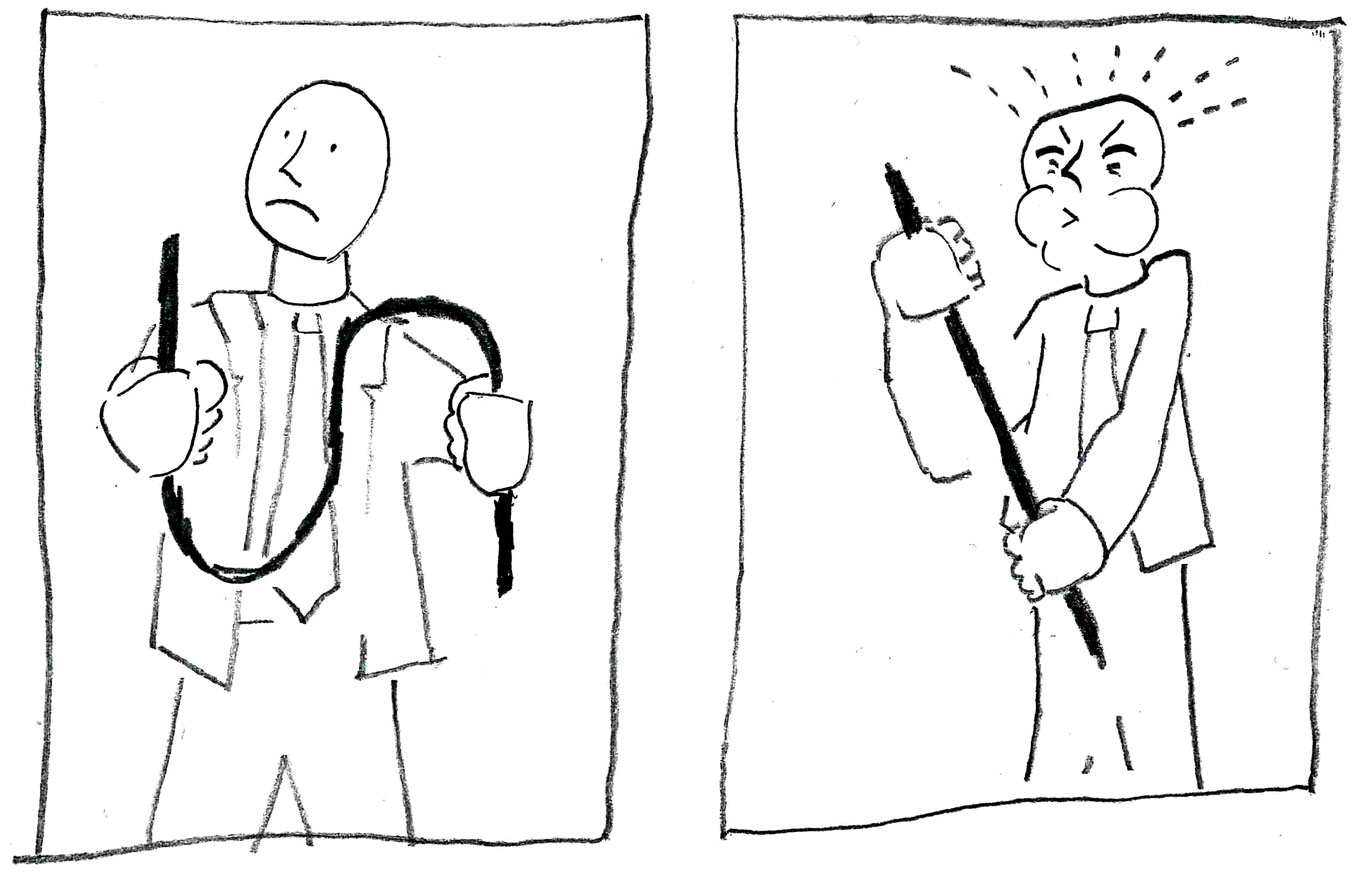
\includegraphics[width=8cm]{yankwire.jpg}
\]
Таким чином, дітсадкова квантова механіка стала реальністю. Такі трюки не були чимось новим, оскільки певному лауреату Нобелівської премії на ім’я Роджер Пенроуз у 1970-х роках так набридло дивитися на індекси в тензорній нотації теорії відносності, що з цією метою він винайшов такого типу зображення. Тож ми були у гарній компанії.

Гарний початок, але скільки корисного можна отримати завдяки таким трюкам? % один трюк?
Ну, як виявилося, багато: можна викладати цілий курс квантових обчислень і квантових основ у цих умовах.\footnote{Цей курс проводиться з 2012 року в Оксфордському університеті, і цей курс став основою для «книги додо». \cite{CKbook}. \href{https://www.cs.ox.ac.uk/teaching/courses/2019-2020/quantum/}{\tt https://www.cs.ox.ac.uk/teaching/courses/2019 -2020/quantum/}}
%quite a lot as we have discovered 
%~\cite{CKbook}. 
Наскількі це дійсно нове? Тобто, чи може малювання квантових процесів дозволити нам робити те, що ми не могли робити раніше? Або це просто арт-проект?

Саме тут з'являється \textit{ZX-числення}.
%\TODOb{There are new things outside of ZX, right?} 
ZX-числення — це графічна мова для вираження квантових обчислень, головним чином над кубітами. Незважаючи на те, що вона існує із 2008 року, справжнє зростання почалося лише в 2018 році, коли з’явилося кілька основних результатів:
 \ben
 \item[(1)] ZX-числення було «завершено», що означає, що всі рівняння, що стосуються квантових процесів із залученням кубітів, які можна вивести за допомогою лінійної алгебри, також можна отримати за допомогою кількох графічних правил \cite{hadzihasanovic2018two, vilmart2019near}. Це об’єднує обіцянки, дані на початку розвитку дитсадкової квантової механіки, що графічне міркування слід розглядати не просто як корисний механізм, а як справжню альтернативу формалізму Гільбертового простору.
 \item[(2)] Для певних задач оптимізації квантових схем,
 %\bR such as ancilla-free T-count reduction\e,\TODOb{This should be a bit broader stated, with less heavy jargon.} 
 методи на основі ZX тепер перевершують найсучасніші, наприклад, ~\cite{de2020fast} показав Т-кількості, які були на 50\% кращі, ніж відомі методи на момент публікації. Ці спрощення важливі для адаптації задач до існуючих квантових комп’ютерів і зіграли важливу роль у розробці комерційних квантових компіляторів, таких як t$|$ket$\rangle$ \cite{sivarajah2020t} Cambridge Quantum Computing.
% \item[(3)] \bR Automated reasoning with the ZX-calculus has been used to verify the correctness of quantum software, and has been 
% %used to find  
% \bB successful at finding\e real bugs in quantum circuits\e.\TODOb{See comments in abstract.} %In order to achieve the latter, \em automated reasoning software \em was used, which in itself is a novelty in theoretical physics.
 \item[(3)] ZX-числення нещодавно дозволив команді перетворити обробку природної мови з урахуванням граматики \cite{CSC} у варіаційні квантові схеми \cite{QNLP-foundations}, придатні для роботи на існуючому маломасштабному квантовому обладнанні, що призвело до першої реалізації квантової обробка природної мови на квантовому комп’ютері \cite{Nature}. %Те саме стосується квантових реалізацій інших графічних теорій.
 \een      
     
Ця стаття не має на меті бути підручником, а є легким вступом і оглядом деяких нещодавніх успіхів.
%, \bR but to provide the reader with an easy-going broad view on the ZX-calculus, with a focus on where it came from, what it is, were it is heading,  and in particular, what it can (now) do for you\e.\TODOb{Is this really what we do here?}
%, hence including its current status, its (potential capabilities), and its background.   
Якщо вам потрібен більш детальний посібник щодо використання ZX-числення, кілька інших ресурсів уже доступні. Наприклад, книга \cite{CKbook} дає розгорнутий вступ до широкої теми пікторальних квантових міркувань, що веде до детального представлення ZX-числення. Незважаючи на те, що це досить великий фоліант (850 сторінок), він повний картинок і його викладали кілька разів (в Оксфорді, Неймегені та Пекіні) приблизно у 20 годинах лекцій. Набагато коротший вступний ZX-посібник це \cite{coecke2012tutorial}, а розширений, актуальний вступ із багатьма прикладами практичної роботи – це ~\cite{JohnSurvey}. Крім того, є підручник для середньої школи \cite{CoeckeGogioso2018}, який ми обговорюємо в розділі \ref{sec:exp}.

%A tutorial on   more broader diagrammatic quantum reasoning is \cite{ContPhys}, and the connections between diagrammatic and category theory are explained in \cite{CatsII, SelingerSurvey}.  
%There also are a number of PhD theses that may be useful depending  one's background \bR e.g.~\cite{}\e.\TODOb{Put some here e.g.~Miriam's}\TODOb{Other stuff useful as tutorials?}
 
%\TODOb{Reconsider at end; we already do a lot of this in the abstract; maybe we don't need any of this and can just KILL.} 
%\bR In Sec.~\ref{sec:whatwhy} we start by explaining what ZX-calculus is, first, in section~\ref{sec:gencomp}, as an example of a compositional process theory, and what the corresponding benefits are, and then, in section~\ref{sec:ZX}, we expose the origin of the power of ZX-calculus  specifically, by comparing it to calculations with quantum circuits. We then address the its universality and completeness, including recipes to translate any matrix into ZX-calculus. We also discuss how ZX-calculus naturally enables automation, and which tools are currently available.
%
%We then move on, in section~\ref{sec:prac}, to the of how ZX-calculus deals with circuit optimisation, and what its achievements are.  Then we move to other practical problems within the context of quantum computing that have been addressed by ZX, and in section~\ref{sec:found} we do the same for some problems in quantum foundations.
% 
%In section~\ref{sec:asmaths}, we discuss the mathematical status of ZX-calculus, and that is a very novel kind of mathematical structure, which only has  started to be studied as such in the past couple of years. We outline the achieved insights of ZX-calculus being a prime example of interacting algebras, and how it compares to the established mathematical structures of Frobenius algebras and Hopf algebras.  
%
%Finally, in section~\ref{sec:whatwhy}, we give an overview of the development of ZX-calculus, including the trajectory towards completeness, the different kinds of rules that have been in the play for that and side tracks (some of which never took off), and one that played a vital role in the quest towards completeness.  This at the same time provides a close-to-complete biography on ZX-calculus.\e

%\section{What and why}\label{sec:whatwhy}%%%%%%%%%%%%   

\section{ZX: LEGO для квантових обчислень}\label{sec:ZX}%%%%%

Ми познайомимося з ZX-численням, порівнюючи його зі стандартною мовою квантових схем, і, зокрема, пояснюючи спосіб, у який ZX-числення (доволі дослівно) виходить за межі того, як ми можемо маніпулювати та міркувати за допомогою квантових схем.

\paragraph{ZX-мова.} Типові примітиви мови квантових схем включають CNOT-вентилі та певні однокубітні вентилі, такі як Z-фазові вентилі та вентиль Адамара. Ми позначаємо їх тут наступним чином:
\[
\tikzfig{cnot}\ \ :=\ \ \left( \begin{matrix}
  1 & 0 & 0 & 0 \\
  0 & 1 & 0 & 0 \\ 
  0 & 0 & 0 & 1 \\
  0 & 0 & 1 & 0
\end{matrix} \right) 
\qquad
\tikzfig{phasegate}\ \ :=\ \  
\left(\begin{matrix}
1 & 0 \\
0 & e^{i \alpha}
\end{matrix}\right) 
\qquad
\tikzfig{Hadamard2}\ \ :=\ \ 
\textstyle{\frac{1}{\sqrt{2}}}  
\left(
\begin{array}{cr}
  1 & 1 \\
  1 & -1
\end{array}
\right)
%\bR \mbox{ZX-notation and corresponding matrix for CNOT, green phase and Hadamard} \e
\]
У той час як Z-фазові вентилем зазвичай вважаються діагональними в стандартному (або "Z") базисі, ми можемо сполучити за допомогою Адамара вентилем, щоб отримати X-фазові вентилі, які є діагональними в Адамаровому (або "X") базисі:
\[
\tikzfig{redphasegate}\ \ :=\ \ \tikzfig{redphasedef} 
%\bR \mbox{red phase from green phase via Hadamard} \e
\]
Ці два типи фазових вентилів тепер можна використовувати для побудови інших речей, наприклад, сам вентиль Адамара тепер з'являється, як скалярний множник (який ми ігноруємо), до \textit{розкладу Ейлера} у термінах фазових вентилів:
\[
\tikzfig{Hadamard2}\ \ =\ \ \tikzfig{HadamardEuler}
%\bR \mbox{Hadamard as Euler} \e 
\]

Замість простого використання стандартних фазових вентилів як будівельних блоків для інших вентилів, ZX-числення використовує їх узагальнення, що дозволяє змінювати кількість вхідних і вихідних проводів цих фазових вентилів. Більш конкретно, ми можемо узагальнити фазові ворота
% \[
% \begin{array}{l}
% \tikzfig{phasegate}\ \ =\ \ \ket{0}\bra{0} + e^{i \alpha} \ket{1}\bra{1}
% \vspace{3mm}\\
% \tikzfig{redphasegate}\ \ =\ \  \ket{+}\bra{+} + e^{i \alpha} \ket{-}\bra{-} 
% \end{array}
% \]
до `павуків':   
\beq\label{eq:spiders}
\begin{array}{l}
\tikzfig{greenspider}\ \ :=\ \ \ket{0\ldots 0}\bra{0\ldots 0} + e^{i \alpha} \ket{1\ldots 1}\bra{1\ldots 1}
\vspace{4mm}\\
\tikzfig{redspider}\ \ :=\ \  \ket{+\ldots +}\bra{+\ldots +} + e^{i \alpha} \ket{-\ldots -}\bra{-\ldots -}
\end{array}  
\eeq
Не вдаючись до бра-кет нотації, Z-павук із $m$ ногами всередині та $n$ ногами назовні є матрицею $2^n \times 2^m$ із рівно 2 ненульовими елементами:
\[
\tikzfig{greenspider}\ \ :=\ \ 
\begin{pmatrix}
  1 & 0 & \cdots & 0 & 0 \\
  0 & 0 & \cdots & 0 & 0 \\
  \vdots & \vdots  & \ddots &  \vdots  &  \vdots  \\
  0 & 0 & \cdots & 0 & 0 \\
  0 & 0 & \cdots & 0 & e^{i\alpha} \\
\end{pmatrix}
\]
і X-павук може бути зроблений з Z-павука так само, як ми робили з фазовими вентилями:
\[
  \tikzfig{redspider} \ \ :=\ \ \tikzfig{Z-color-ch}
\]

Відсутність $\alpha$ означає $\alpha = 0$, напр.
\[
\tikzfig{greenspider0}\ \ :=\ \ 
\begin{pmatrix}
  1 & 0 & \cdots & 0 & 0 \\
  0 & 0 & \cdots & 0 & 0 \\
  \vdots & \vdots  & \ddots &  \vdots  &  \vdots  \\
  0 & 0 & \cdots & 0 & 0 \\
  0 & 0 & \cdots & 0 & 1 \\
\end{pmatrix}
\]
Звідси випливає, що чашки та шапки (\ref{eq:cupcap}), а також багато основних квантових станів і ефектів є окремими випадками павуків:
\ctikzfig{basic-spiders}
де $\ket{{+}} = 1/\sqrt{2} \big(\ket 0 + \ket 1\big)$, $\ket{{-}} = 1/\sqrt{2} \big(\ket 0 - \ket 1\big)$, ми проігнорували деякі фактори нормалізації.

Павуки - це все, з чого складається мова ZX-числення. Чому ZX-числення може обійтися тільки цим?
Оскільки тепер ми можемо побудувати CNOT-вентилі з цих павуків наступним чином:
\beq\label{cnotfromspiders}
\tikzfig{cnotfromspiders}
\eeq
Те, що це справді так, можна легко перевірити за допомогою матриць. Так, зокрема, CNOT-вентиль більше не потрібно розглядати як примітив, він розпадається на дві менші частини. Коли у нас є фазові вентилі та CNOT-вентилі, ми знаємо, що можемо відтворити будь-яку квантову схему, що складається з будь-яких вентилів.

Який результат цього? Точніше, чому це краще, ніж використання стандартних схем?
Справжня сила ZX-числення полягає в тому, що з цими меншими частинами в (\ref{cnotfromspiders}) дуже легко працювати, у тому сенсі, що правила, які ними керують, легко зрозуміти, запам’ятати та виконати обчислення за ними. Крім того, їх не так багато. Навпаки, придумати всі правила, які керують фіксованим набором квантових вентилів, справді важко, і мало що відомо, окрім випадків дуже обмежених наборів воріт~\cite{cnotdihedral} або невеликої фіксованої кількості кубітів.

Наприклад, було показано в~\cite{ptbian}, що \textit{дійсно} існує набір правил рівнянь квантових схем, яких достатньо, щоб підтвердити всі істинні рівняння для 2-кубітових схем, побудованих із цих вентилів:
\[
\tikzfig{phasegateT}\qquad\qquad\qquad\tikzfig{Hadamard2}\qquad\qquad\qquad\tikzfig{cnot}  
\]
Це вентилі, які ми представили на початку цього розділу, але з Z-фазами, обмеженими $\alpha = \pi/4$.
Однак деякі правила величезні, і з ними важко працювати. Цілком їх можна знайти в ~\cite{DBLP:conf/rc/CoeckeW18}, але щоб відчути їхній масштаб, ось ліва частина одного з правил, яка завелика, щоб поміститися на сторінці :
\beq\label{circ:completerelationlist142}
\tikzfig{completerelationlist142} 
\eeq

% Why did we start with the 2-qubit case?  Since this is the only one where the rules for the circuits are even known.  We are not going to write all the rules down here (which were identified in \cite{ptbian}, and can be found in \cite{DBLP:conf/rc/CoeckeW18}), but simply point out that the circuit (\ref{circ:completerelationlist142}) above appears in one of the rules, just to make the point that they are impossible to remember, let alone calculate with.  

% We are pretty confident about the following two conjectures.  
%So confident even that we really haven't put any effort in trying to prove them.

Ми очікуємо, що ця ситуація погіршуватиметься, коли ми переходимо до більшої кількості кубітів. Наприклад, важко уявити, що таке подальше 3-кубітне правило, як:
\begin{equation}\label{eq:3qubit}
\tikzfig{CNOT-Frob}
\end{equation}
можна коли-небудь підтвердити, використовуючи лише 2-кубітні правила із \cite{ptbian, DBLP:conf/rc/CoeckeW18} або будь-якіх 2-кубітні правила власне кажучи. Здається, що для цього потрібно розкласти принаймні один із вентилів CNOT на однокубітні вентилі, що неможливо. Звичайно, диявол криється в деталях, тому поки що залишимо наступне як припущення:

\begin{conj}
  Жоден набір правил, що включає лише дві схеми кубітів, не може бути повним для схем із більш ніж 2 кубітами.
\end{conj}

З іншого боку, ми побачимо в розділі про повноту~\ref{sec:compl}, що можна розмістити на одній стороні A4 усі ZX-правила, необхідні для доведення всіх рівнянь, які є вірними для для всіх ZX-картинки, включаючи схеми, створені з будь-яких вентилів з будь-якою кількістю кубітів.

% \noindent
% {\bf Proof suggestion.} Show that no rules for 2 qubits could ever be used to derive this rule: 
% \ctikzfig{CNOT-Frob}
%which as we will see below, corresponds to a standard ZX-calculus rule.

%\par\bigskip\noindent
% As already mentioned, beyond 2 qubits very little is known for quantum circuits, and one would expect that if anything can be shown, it would be incredibly complicated, as, at the very least it will have to subsume the already very complicated 2 qubit rules. 

% On the other hand, not only are the ZX-rules for the 2-qubit  Clifford+T circuits easy and simple, in fact, they essentially extend to all quantum circuits, not just  Clifford+T  but all of them, and especially, not just 2-qubit but all of them, and even more, they extend to all linear maps. So case closed as far as equational reasoning for quantum theory is concerned!
 
%\bR ... we explain the rules below ... \e

Ці набагато простіші ZX-правила відображають той факт, що ZX-мова тим чи іншим чином більш фундаментальна, ніж схеми.

% To make an analogy with particle physics: 
% \begin{center}
% \em ZX-calculus `splits the atom' of the circuit model of quantum computing.\em
% \end{center} 
% So one could say that ZX-calculus reveals the true fundamental particles of quantum computing.
%Once done so, \bR we can use them in a fusion reactor\e.\TODOb{This can probably be improved upon still.}

Розглянемо аналогію з LEGO. Базову цеглинку LEGO було розроблено для її універсальності, але якщо ви були настільки божевільні, щоб склеїти всі свої LEGO разом у кілька фіксованих «композитних» блоків, ця знаменита універсальність зникає. Просто заради розваги, давайте розглянемо це трохи далі і припустимо, що справді існують аналоги LEGO для зображень ZX:
\begin{center} 
\begin{tabular}{|c|c|}
\hline
{\bf ZX-мова}  & {\bf LEGO аналогія}\\ 
 \hline \hline
\tikzfig{phasegate_table} \qquad\quad\  \tikzfig{redphasegate_table}  & \raisebox{-6mm}{\epsfig{figure=images-sm/Lego-single1,width=140pt}}\\ 
 \hline
\tikzfig{phasecirc_table}  & \raisebox{-8.5mm}{\epsfig{figure=images-sm/Lego-phasecirc,width=140pt}}\\  
 \hline
\raisebox{2mm}{\tikzfig{copy_table}} \qquad \raisebox{2mm}{\tikzfig{redcopy_table}} & \raisebox{-6mm}{\epsfig{figure=images-sm/Lego-double1,width=140pt}}\\ 
 \hline
\raisebox{3mm}{\tikzfig{cnot_table}}  & \raisebox{-6mm}{\epsfig{figure=images-sm/Lego-crossed1,width=140pt}}\\
 \hline 
\end{tabular}
\end{center}
Стандартний LEGO дозволяє створювати безліч творів:
\[
  \epsfig{figure=images-sm/house1,width=140pt}
\]
тоді як композитний блок допускає лише обмежений спектр «мистецтва»:
\[
  \epsfig{figure=images-sm/art,width=220pt}
\]
Зокрема, схемні вентилі мають унітарність, а ZX-компоненти звільнені від унітарного обмеження.

Якщо ми хочемо фактично запустити обчислення на квантовому комп’ютері, може статися так, що зрештою нас дійсно цікавлять лише унітарні квантові схеми. У такому випадку природно запитати: чи справді ця додаткова свобода \textit{гарна} річ? Ми б стверджували, що це так, і що ми маємо ситуацію, яка дещо схожа на комплексний аналіз.
У випадку складного аналізу, залишення дійсних чисел позаду (іноді тимчасово) дає нам набагато більше потужності та елегантності, навіть коли ми доводимо речі про дійсні числа. Ми побачимо, що це саме явище відбувається для ZX-зображень у Розділі~\ref{sec:circoptim}, де ми обговорюємо, як оптимізувати квантові схеми шляхом тимчасового виходу зі світу схем, а потім повернення.

Було пояснено в~\cite{GLAmagiclego}, що алгебраїчні структури, які лежать в основі ZX-числення, — це не просто звичайний LEGO, а «чарівний LEGO», який є дуже гнучким і дозволяє створювати всі види нестямний творінь. Це завдяки гнучкості графічної мови, яку ми обговоримо в наступному розділі. Розглядаючи лише «склеєні» LEGO, тобто квантові вентилі, ми пропускаємо всю цю історію. Отже, мораль така:
\begin{center}
  \it Припиніть склеювати своє LEGO!
\end{center}

\section{Базові ZX-правила}

\paragraph{Правила злиття павуків.} Конкретно, існує три типи правил, які керують павуками ZX (\ref{eq:spiders}). Перший тип стосується того, як взаємодіють павуки одного кольору, і вони дуже прості: павуки одного кольору «зливаються» разом, і їхні фази складаються:
\beq\label{eq:spider-fusion}
\tikzfig{spiderphaseg}\ \ =\ \ \tikzfig{spidercompphaseg}  
\qquad\qquad\qquad
\tikzfig{spiderphaser}\ \ =\ \ \tikzfig{spidercompphaser}
\eeq

Один із способів уявити павуків як «багато-дротових», оскільки звичайні дроти мають два кінці, багато-дроти можуть мати декілька кінців. Тоді наступні багато-дроти є звичайними дротами:
\[
\tikzfig{ordinarywire}  
\]
Що характеризує дріт, так це те, що він з’єднує два кінці, і якщо ви з’єднаєте два дроти разом, ви знову отримаєте (тепер довший) дріт. Те саме стосується багатодротових мереж, і (\ref{eq:spider-fusion}) просто говорить, що якщо ви з’єднаєте два багатодротові мережі, ви отримаєте ще одну багатодротову мережу.

Також немає реальної різниці між вхідною-лапкою-павука і вихідною-лапкою-павука, оскільки злиття-павуків дозволяє легко міняти ці ролі:
\[
\tikzfig{ordinarywire2}  
\]
Загалом це означає, що в ZX-численні:
\begin{center}
\em  має значення тільки зв'язок
\end{center}
і що ми можемо думати про ZX-картинки як про графи, тобто щось, що визначається вузлами та ребрами, що їх з’єднують. Тоді незв'язані ноги роблять його «відкритим» графом \cite{DK}. Ця гнучкість не має сенсу для звичайних схем, де кожен вентиль повинен мати чітко визначені входи та виходи.

\paragraph{Сильні правила комплементарності.}  Другий тип правил стосується взаємодії між павуками різного кольору.
Їх можна сформулювати як ці два правила:  
\beq\label{eq:bialg1}
\tikzfig{bialg1} 
\eeq
разом із цим третім:
\beq\label{eq:bialg2}
\tikzfig{bialg2} 
\eeq 
або, як це єдине правило:
\beq\label{eq:bialg3}
\tikzfig{bialg3} 
\eeq
Правила (\ref{eq:bialg1}) говорять нам, що одноногі павуки (а.к.а.~стани/ефекти) копіюються павуками протилежного кольору. Правило (\ref{eq:bialg2}) трохи важче інтерпретувати, і навіть не будемо починати про (\ref{eq:bialg3}).
Але всі вони слідують чіткому шаблону, а саме, різні кольори можуть рухатися один через одного. Взявши ці правила разом із злиттям-павуків, можна вивести таке \cite{CD2}:
\beq\label{eq:bialg4}
\tikzfig{bialg4} 
\eeq
Давайте ще раз підкреслимо, що для виведення цього правила важливо мати злиття-павуків. Без нього (\ref{eq:bialg3}) і (\ref{eq:bialg4}) незалежні. Насправді в математиці правило (\ref{eq:bialg3}) визначає біалгебру, а наявність (\ref{eq:bialg4}) робить її алгеброю Хопфа (з тривіальним антиподом) \cite{cartier2007primer}. Ми скажемо більше про математичну звичність цих конкретних правил у Розд.~\ref{sec:furtherrefs}. 

Правило (\ref{eq:bialg4}) має дуже інтуїтивне читання, а саме те, що два дроти між павуками протилежного кольору завжди зникають. Іншими словами, 2-цикл завжди зникає:
\[ 
\tikzfig{2loop}
\]
Ми також можемо дати аналогічну інтерпретацію (\ref{eq:bialg2}), а саме, що ми також можемо виключити всі 4-цикли:
\[ 
\tikzfig{4loop}
\]

Правило (\ref{eq:bialg4}) також має дуже чітке концептуальне тлумачення, а саме комплементарність або, за сучасною термінологією, неупередженість. Можна показати, що павуки, визначені як лінійні карти, які підкоряються злиттю-павуків, завжди однозначно фіксуються вибором ортонормованого базису~\cite{CPV}. Тоді (\ref{eq:bialg4}) говорить нам, що ці два ортонормальні бази мають бути взаємно неупередженими \cite{CD2, CKbook}. Взаємно неупереджені основи постійно виникають у квантових обчисленнях і квантовій теорії інформації. Наприклад, багато квантової криптографії, включаючи знаменитий протокол квантового розподілу ключів BB84~\cite{BB84}, залежить від взаємно неупереджених баз.

Отже, правило (\ref{eq:bialg4}) визначає пари взаємно неупереджених ортонормальних баз. Оскільки, припускаючи злиття павуків, правило (\ref{eq:bialg3}) сильніше ніж (\ref{eq:bialg4}), ми називаємо це «сильною комплементарністю». Цікава річ у цьому новому понятті сильної комплементарності полягає в тому, що ми насправді знаємо про неї більше, ніж про звичайну комплементарність. Ми знаємо, що взаємна сильна комплементарність є моногамною, тому вона може бути лише парами \cite[Thm.~9.66]{CKbook}, і всі ці пари були повністю класифіковані для скінченновимірних гільбертових просторів у термінах скінченних абелевих груп \cite{CDKZ}.


З точки зору схем, правило (\ref{eq:bialg4}) говорить нам, що CNOT-вентилі є унітарними:
\[ 
\tikzfig{unitarity}
\]
Якщо замість CNOT-вентилей, що діють на той самий дріт однакового кольору, ми зробимо навпаки, ми отримаємо інтерпретацію схеми для (\ref{eq:bialg2}):
\[ 
\tikzfig{strongcomplementary1CNOT}
\] 
Разом ці два рівняння схем дають:
\[ 
\tikzfig{3-cnot-swap}   
\] 

Більш широке обговорення сильної комплементарності міститься в \cite{CKbook}. Наразі ми припиняємо обговорювати правила, а виконаємо деякі речі з тими правилами, що є. Ми обговоримо правила далі в наступному розділі.

\section{Повне числення}\label{sec:compl}%%%%%

Ні правила (\ref{eq:spider-fusion}), ні (\ref{eq:bialg3}) не є специфічними для кубітів, але мають сенс у всіх вимірах і навіть за межами квантової теорії Гільбертового простору. Дійсно, вони створюють канву для вивчення теорій, більш загальних, ніж квантова теорія, і вони, наприклад, уможливили чітке графічне представлення теорії іграшок Спеккенса \cite{CEToy, CES, MiriamSpek}. Примітно, що такий вид презентації дозволяє точно визначити, де квантова теорія та цікаві «квантовоподібні» теорії відділяються. У цьому випадку це пов’язано з різницею у двох скінченних групах $\mathbb{Z}_4$ і $\mathbb{Z}_2\times\mathbb{Z}_2$. Широке обговорення всього цього міститься в \cite{CKbook}, Розділ 11.

Інші статті про узагальнені теорії, засновані на сильній комплементарності, включають \cite{CDKZ, gogioso2015schroedinger, gogioso2015fourier, CDKZ2, gogioso2019diagrammatic, gogioso2019generalised}. Усе це є частиною підходу «процесних теорій» до квантових основ, де квантовоподібні теорії визначаються за допомогою симетричної моноїдальної категорії, так само як теорія процесів, а їхні особливості вивчаються абстрактно (див., наприклад, ~\cite{JTF, selby2017leaks, gogioso2018categorical, gogioso2018density, selby2018reconstructing, lee2018no,coecke2016terminality, kissinger2017categorical, pinzani2019categorical, pinzani2020giving}).

Однак, якщо ми повернемося на землю, ми зможемо подивитися, які правила насправді \textit{є} специфічними для квантових обчислень з кубітами. Як ми побачимо, нам не потрібно заходити надто далеко, перш ніж матимемо достатньо правил, щоб довести кожне справжнє рівняння між малюнками.

% quantum causal process structures as a topic of particular interest \cite{coecke2016terminality, kissinger2017categorical, pinzani2019categorical, pinzani2020giving}.  

\paragraph{Правило(-а), пов’язані з кубітом.}  Знову звертаючи нашу увагу на гільбертовий простір і кубіти конкретно, ще одне правило, яке було частиною ZX-числення на ранньому етапі, хоча й у зовсім іншій формі, це таке:
\beq\label{spider-convert1}
\tikzfig{spider-convert1}   
\eeq
Форма, у якій воно з’явилося спочатку, була першим із цих правил \cite{CD1}:
\beq\label{hbox-colour-change}
\tikzfig{hbox-colour-change}   
\qquad\qquad\qquad\qquad
\tikzfig{Hadamard2}\ \ =\ \ \tikzfig{Hadamard-euler-single1}  
\eeq
який є гарним, а друге додано трохи пізніше \cite{duncan2009graph}, який є трохи менш гарним. Разом ці два правила, що стосуються жовтої рамки, еквівалентні (\ref{spider-convert1}). Отже, що нам говорить {(\ref{spider-convert1})?

Ми вже розповідали вам про X-павуків і Z-павуків, але ви можете запитати, «що трапилося з Y?» Ми поклали свої мізки в піч і спекли наші Y?

Ні! Насправді ми не визначали Y-павуків, тому що їх уже можна визначити двома різними способами: у термінах X-павука або в термінах Z-павука. Рівняння~\eqref{spider-convert1} пов’язує ці два різні способи.

Це правило походить від геометрії \textit{сфери Блоха}, загального способу візуалізації операцій кубіта як обертання сфери, щоб обертати X/Z на Y. Крім того, ви можете трохи змінити це правило наступним чином:
\[
\tikzfig{spider-convert2}    
\]
що насправді:
\[
\tikzfig{spider-convert3}    
\]
А, отже-сенько, еквівалентність із правилами (\ref{hbox-colour-change}). Перегляньте \cite{CKbook} для належного доказу, без `сенько'. :)

\paragraph{Повний набір правил}  Отже, що ми можемо довести за правилами, які ми маємо зараз? Це:
\begin{equation}\label{stabrules}
\tikzfig{AllRules}
\end{equation}
Ми вже зазначали в Розділі \ref{sec:ZX}, що за допомогою ZX-числення ми можемо пройти весь шлях і довести кожне рівняння, яке можна довести за допомогою лінійної алгебри. У \cite{VladComp} було показано, що цих правил поки недостатньо.

Проте Бекенс~\cite{Backens} показав, що вони дають нам змогу довести кожне рівняння, яке виконується для \textit{квантової теорії стабілізатора}, тобто ZX-зображень із фазами, кратними $\pi/2$.

% This is, informally, qubits being restricted to only having 6 states, namely the Z-, X- and Y- eigenstates.  In terms of ZX-calculus, this means that there only are phases that are multiples of ${\pi\over 2}$:
% \beq\label{eq:stabphase}
% \tikzfig{stabphase}
% \eeq  

Це, звичайно, не маловажливий фрагмент квантової теорії, оскільки, наприклад, достатньо довести, що квантова теорія є нелокальною \cite{CDKZ}. З іншого боку, квантові схеми стабілізатора можна ефективно моделювати класично \cite{GottesmanKnill}.
%Perhaps unsurprisingly, the ZX-rules above can not only prove all true equations between stabiliser ZX-pictures, they can do it efficiently.

% But still, for many practical applications involving circuits that cannot be simulated, these stabiliser ZX-rules are sufficient for the job.

%Going beyond stabiliser ZX-pictures, we get into a realm of things that cannot be classically simulated.

На практиці, навіть незважаючи на те, що наведені вище ZX-правила не можуть підтвердити \textit{всі} рівняння, включаючи схеми за межами квантової теорії стабілізатора, вони здаються досить придатними для багатьох практичних завдань, таких як оптимізація схем, як ми побачимо в наступному розділі. % у цьому випадку правила виглядають досить

Звичайно, ми дійсно хочемо зрозуміти, які додаткові правила потрібні, щоб мати можливість довести всі рівняння. Вони були вперше встановлені Нг та Вонг у \cite{ng2017universal}, спираючись на результат Хадзіхасановича щодо графічного числення, пов’язаного із ZX-численням \cite{hadzihasanovic2017algebra, hadzihasanovic2018two}. По дорозі результат Жанделя, Пердрікса та Вілмарта встановив можливість виводу всіх рівнянь для `Кліффорд+Т' ZX-зображень, які узагальнюють стабілізатори, допускаючи кратні $\pi/4$, а не лише $\pi/2$ ~\cite{jeandel2018complete}.

Подібні теореми називають теоремами \textit{про повноту} в тому сенсі, що правила утворюють повний набір щодо можливості виведення. Зараз існує кілька різних повних наборів правил для повного сімейства ZX-зображень ~\cite{ng2017universal,vilmart2019near}, а також для різних спеціальніх випадків~\cite{jpvnormalform,jeandel2018complete,jeandel2018diagrammatic,zxtri}. Найбільш стислий набір на даний момент додає єдине правило до 4 правил вище, яке дозволяє обмінювати кольори фаз у трійках \cite{vilmart2019near}:
\beq\label{colour-change-rule} 
\tikzfig{Renaut} 
\eeq
де кожна з фаз $\tilde\alpha, \tilde\beta, \tilde\gamma$ є тригонометричними функціями фаз у лівій частині.

Це правило вперше було введено для випадку двокубітових схем \cite{DBLP:conf/rc/CoeckeW18}, причому двоє авторів цієї статті не зрозуміли, що це також дасть повномасштабну повноту. Здається, це показує нам, що чотири основні правила \eqref{stabrules} вже охоплюють усі складні взаємодії кількох кубітів, аж до деяких «локальних» одиничних рівнянь кубітів, які всі поглинаються ~\eqref{colour-change-rule}.

Отже, якщо ми маємо повний набір правил для всіх ZX-зображень, ми повинні бути щасливі, чи не так? Неправильно! Повнота повинна розглядатися як початок, а не кінець для обчислення ZX, і можна багато чого отримати, знайшовши кращі правила.
 
Наприклад, стислість, отримана завдяки введенню правила зміни кольору (\ref{colour-change-rule}), коштує введення складних тригонометричних функцій фаз кожного разу, коли воно застосовується. Насправді вони досить потворні, тому ми навіть не потрудилися написати їх тут. Якщо ми працюємо з фазами чисельно на комп’ютері, це не є великою проблемою, але для символічних маніпуляцій це швидко стає непрактичним.

Один із способів вирішення цієї проблеми — перейти до \textit{алгебраїчного ZX-числення}, яке замінює фази $\alpha \in [0,2\pi)$ -- які стають $e^{i\alpha}$ у визначення павука \eqref{eq:spiders} -- на прості комплекснимі числа $a \in \mathbb C$:
\[
\tikzfig{greenspider} \qquad\qquad\leadsto\qquad\qquad  \tikzfig{greenboxspider}
\]
Наше попереднє уявлення про павуків все ще існує, просто встановивши $a := e^{i\alpha}$, але додаткова загальність дає нам кілька приємних особливостей, таких як більш просте кодування комплексних матриць, також як і прямолінійне узагальнення від 2D до всіх скінченних вимірів~\cite{qwangslides} і від комплексних чисел до будь-якого комутативного півкільця~\cite{azxsemiring}.
 
\section{Автоматизована оптимізація схем}\label{sec:circoptim}%%%%% 

Якщо задано схему, чи може ZX-числення допомогти її спростити? Звичайно, може, і, здається, вдається йому краще за будь-що інше. Ось приклад того, як це працює. Припустімо, ми хочемо спростити наступну схему, що складається з кількох вентилів, і нам потрібно виміряти останні два кубіти:
\[
\tikzfig{q_circuit_new}
\]
Тут є багато 4-циклів, і ми щойно дізналися, що ZX-числення добре позбавляється від 4-циклів. 4-цикли тут:
\[ 
\tikzfig{QC1}    
\] 
Однак вони не є 4-циклами, тому що вони виглядають як прямокутники, оскільки 4-цикли, які ми шукаємо, мають чергування кольорів як кути. Ми можемо зробити деякі (роз-)злиття:
\[ 
\tikzfig{QC2}    
\] 
і тепер ми можемо видалити цей квадрат, а потім трохи переставити:
\[ 
\tikzfig{QC3}    
\] 
Ми можемо зробити те саме для інших 4-циклів:
\[ 
\tikzfig{QC4}    
\] 
Те, що ми отримуємо, було названо «фазовим гаджетом»~\cite{KissingerTcount}. Знову використовуючи трюк для усунення 4-циклів, можна також виявити, що фазові гаджети з протилежними кутами компенсуються:
\[ 
\tikzfig{QC6}      
\] 

Гей-гоп поїхали. Спочатку вводимо фазові гаджети, а потім зливаємо:
\[
\tikzfig{q_circuit_new_reduce} 
\]
Ми отримуємо 2-цикл, який, як ми знаємо, зникає, а потім два кубіти ліворуч повністю відокремлюються від кубітів праворуч, тому ми можемо про них забути:
\[
\tikzfig{q_circuit_new_reduce1}  
\]
в результаті ми отримуємо те, з чого почали, незважаючи на те, що коли ми починали схема виглядала досить складною.

Незважаючи на те, що легко працювати з невеликими схемами вручну, ми також хотіли б застосувати ці методи до схем із тисячами або мільйонами квантових вентилів, тому природно подумати про те, як такі види спрощень можна автоматизувати. Стандартним методом для цього є заміна рівнянь, які можна застосовувати в будь-якому напрямку, на спрямовані правила перезапису. Наприклад:
\beq\label{eq:rewrite-rule}
\tikzfig{spiderphaseg}\ \ =\ \ \tikzfig{spidercompphaseg}  
\qquad\qquad\leadsto\qquad\qquad
\tikzfig{spiderphaseg}\ \ \rightarrow\ \ \tikzfig{spidercompphaseg}   
\eeq
Поки правила зменшують деякі показники ZX-зображення (наприклад, ~кількість павуків), застосування їх наосліп, доки вони не перестануть застосовуватися, завжди завершується. На жаргоні теорії перезапису це означає, що ми можемо автоматизувати спрощення ZX-зображень за допомогою \textit{системи завершення перезапису}, заснованої на підмножині правил ZX-числення.

Це переписування можна формалізувати таким чином, щоб ZX-зображення могли бути представлені та трансформовані програмними інструментами за допомогою методу під назвою \textit{переписування графа з подвійним висуванням}~\cite{dpo-old}. Базова теорія для представлення ZX-зображень у вигляді графів і їх переписування була представлена в ~\cite{DK} і нещодавно розширена в~\cite{bonchi2020string}. Це формує основу діаграмного `помічника з доказів' під назвою Quantomatic~\cite{quanto-cade}.


% \TODOb{Some screenshots would be nice here.} \COMMh{Maybe just mention PyZX as an optimisation tool here? Because ours is just an algorithm implemented in Haskell code which just works for T-count reduction.} 

«Розриваючи» вентилі в квантовій схемі, ми можемо знайти спрощення в ZX-численні, які були б приховані на рівні вентиля. Однак ми можемо отримати щось, що більше не буде схоже на схему. Отже, важливою проблемою для методів оптимізації на основі ZX є \textit{вилучення схеми}, яке ефективно відновлює вентильну декомпозицію зі спрощеного ZX-зображення. Ця техніка спрощення та виділення для ZX була введена в~\cite{clifford-simp}, узагальнена до ширшого сімейства діаграм у~\cite{backens2020there} та є основою інструменту квантової оптимізації схеми PyZX~\cite {pyzx} (Рис.~\ref{fig:pyzx}).

\begin{figure}[]
  \centering
  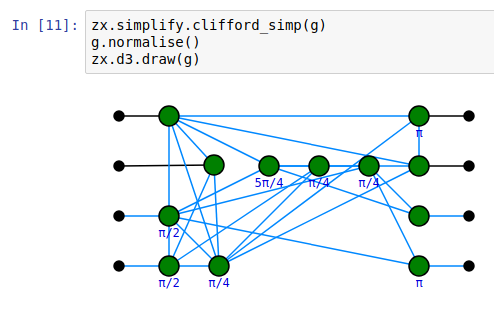
\includegraphics[width=0.7\textwidth]{pyzx2.png}
  \caption{PyZX — це бібліотека Python і інструмент оптимізації схем за допомогою ZX-числення. Дивись \url{github.com/Quantomatic/pyzx}.}
  \label{fig:pyzx}
\end{figure}


Перезапис ZX-зображеннь також є основою спеціального інструменту спрощення схеми STOMP \cite{de2020fast}, який зменшує важливу метрику вартості, звану Т-кількістю квантової схеми, використовуючи так звані ідентичності «павукових гнізд».


\section{Квантова обробка природної мови}\label{sec:QNLP}%%%%%   

ZX-обчислення виникло з більш загального образного підходу до квантових основ і квантового числення, що називається категоріальною квантовою механікою (CQM) \cite{AC1, Kindergarten}. Насправді CQM пропонує альтернативний гільбертовому простору формалізм, який робить наголос на тому, як складаються системи, а не на тому, в якому просторі системи описуються. Завдяки успіхам ZX-числення можна справедливо сказати, що ця альтернатива має справжні практичні переваги.

З іншого боку, графічні структури, які використовує CQM (і в багатьох випадках походять звідти), виходять далеко за межі квантової теорії. Наприклад, вони були застосовані в
теорія обчислюваності~\cite{pavlovic2013monoidal}, моделі паралелізму~\cite{Sobocinski:2010aa}, теорія керування~\cite{Baez2014a,Bonchi2015}, дослідження електричних~\cite{BaezFongElec} та цифрових~\cite{GhicaCircuit} схеми, теорія ігор~\cite{ghani2016compositional}, ширші когнітивні функції \cite{ConcSpacI}, обробка природної мови \cite{CSC, FrobMeanI} і навіть дослідження свідомості \cite{seanconscious, wangconscious}!

Оскільки аспекти ZX-обчислення є важливими для деяких із цих областей, можна стверджувати, що певною мірою вони є «кванто-подібними». Хоча в деяких випадках це можна сприймати лише як приблизну аналогію, у конкретній області обробки природної мови (ОПМ) здається корисним сприймати цей квантовий зв’язок серйозно. У підході до ОПМ, запропонованому в~\cite{CSC}, моделі векторного простору для значення слова були об’єднані з граматичною структурою для створення композиційних моделей значення речення. Оскільки ця модель дуже важливо використовує цей тензорний добуток векторних просторів, що дає експоненціальні вимоги до простору на класичному комп’ютері. З іншого боку, формування тензорних добутків на квантовому комп’ютері є дешевим, оскільки це саме те, що відбувається, коли ви розміщуєте два фрагменти квантових даних поруч. Це усвідомлення призвело до пропозиції квантового алгоритму обробки природної мови~\cite{WillC}. З різних причин ця перша пропозиція була не дуже практичною для роботи на квантових комп’ютерах сьогодні чи найближчого майбутнього.

%In particular, the approach to natural language processing put forward in~\cite{CSC, FrobMeanI} makes essential use of the tensor product of Hilbert spaces, and this happens to be something that is not easy to simulate on classical computers, as it results in an exponential blow-up of space requirements. % Also, known quantum algorithms may be adjusted to relevant tasks in these areas.  

% This has already been realised for one area in particular, namely natural language, and its computational counterpart natural language processing in particular \cite{WillC}.

% Earlier work combined (i) models for natural language meaning, with (ii) models for grammar, within a quantum-like model \cite{CSC}, something that hadn't been established before---except for true/false-meaning.  However, this model came at an exponentially expensive space cost, just like when simulating quantum systems, a cost that vanished when implementing it on a quantum computer.  It also enjoyed quantum algorithmic speed-up.

Нещодавно цю пропозицію було скориговано та вдосконалено, щоб відповідати існуючому квантовому апаратному забезпеченню \cite{QPL-QNLP, QNLP-foundations}, і реалізовано на квантових пристроях IBM~\cite{Nature}. Це стало прикладом «нативно-квантового» рішення класичної проблеми. Тобто, хоча проблема не має нічого спільного з квантовими системами, її структура все ще природно живе на квантовому комп’ютері.


Важливим удосконаленням від оригінального алгоритму до того, який нещодавно реалізовано на реальному квантовому комп’ютері, було використання ZX-числення для перетворення зображення, що представляє речення природної мови, у квантову схему, що виконується, яка обчислює щось про значення речення в рамках моделі NLP. Ось приклад речення та його інтерпретація як зображення:
\[
\llbracket \textrm{{\tt Alice hates Bob.}} \rrbracket \ \ =\ \ \ 
\tikzfig{tv3}  
\]
Щоб «запустити» це речення на квантовому комп’ютері, ми спочатку інтерпретуємо чорну крапку як зеленого ZX-павука. Тепер ми можемо використовувати ZX-числення, щоб перетворити його на схему:
\[
\tikzfig{tv4}
\]
Потім ми можемо використовувати правила ZX-числення, щоб масувати цю діаграму в іншу форму (із еквівалентним значенням):
\begin{equation}\label{eq:elastic}
\tikzfig{tv12}
\end{equation}
і замініть значення слів деякими фрагментами ZX-картинки з вільними параметрами, $\alpha, \beta, ...$:
\[
\tikzfig{tv17more}
\]
Ці параметри «навчаються» протягом багатьох прогонів таких схем за допомогою методів машинного навчання. Кінцевий продукт — це квантова схема, здатна в принципі порівнювати значення речень, відповідати на запитання та виконувати багато інших лінгвістичних завдань.

Це дуже просте речення використовує лише дрібку ZX-числення, але вже стає зрозуміло, що «еластичність» ZX корисна для таких завдань. Існує багато еквівалентних способів обчислення значення речення, і деякі краще підходять для квантового комп’ютера, ніж інші, тому «масаж» у рівнянні~\eqref{eq:elastic}. Це дійсно починає окупатися, коли ви починаєте розглядати більш складні речення, як це:
This very simple sentence only uses a dash of ZX-calculus, but it already becomes clear that the `elasticity' of ZX is helpful for such tasks. There are many equivalent ways to compute the sentence meaning, and some fit better on a quantum computer than others, hence the `massaging' in equation~\eqref{eq:elastic}. This really starts to pay off when one starts to consider more complex sentences like this one:
\[
\tikzfig{relpronEduardo} 
\]
Це можна розглядати як процес компіляції, але такий, який приймає не мову програмування як вхідні дані, а природну мову, і перетворює його на квантовий машинний код за допомогою ZX-числення для обробки всього проміжного. Кінцевим результатом є фізика: використання квантових систем для обробки природної мови за допомогою ZX-числення.

Квантове машинне навчання відіграє центральну роль у квантовій обробці природної мови. Останнім часом ZX-числення почало відігравати важливу роль у покращенні нашого розуміння самого квантового машинного навчання: спочатку у зображенні квантового ans\"atze~\cite{yeung2020diagrammatic}, а потім в аналізі важливих проблем у підході, таких як феномен безплідного плато~\cite{zhao2021analyzing}.

\section{MBQC і відмовостійкість}\label{sec:prac}%%%%%%%%%%%%     
     
Квантові обчислення на основі вимірювань (MBQC від Measurement-based quantum computing) — це модель обчислень, альтернативна схемній моделі, де вимірювання, а не квантові ворота, є основними елементами, що керують обчисленнями. Найбільш добре вивчена конфігурація MBQC називається квантовою \textit{односторонньою моделлю}~\cite{MBQC2}. У цій конфігурації багато кубітів готуються в певному фіксованому стані, що називається \textit{станом графа}, а потім одно-кубітовими вимірюваннями готуються у певному порядку.

Примітно, що вибір типу виконаного вимірювання може залежати від попередніх результатів вимірювання, принцип, який називають \textit{передаючим}. Незважаючи на те, що кожен окремий результат вимірювання є недетермінованим, розумне застосування прямого зв’язку може створити детерміновані квантові обчислення.

Наприклад, в односторонній моделі вимірювання визначаються кутами $\alpha \in [0, 2\pi)$. Коли вони виконуються, відбувається одна з двох недетермінованих речей:
\[ \tikzfig{alpha-effect} \textrm{\quad або \quad} \tikzfig{alphapi-effect}. \]
Припустімо, що ми справді хотіли отримати перший результат для нашого обчислення, тоді обчислення ZX підказує нам, як «просунути» небажаний $\pi$ вперед у часі, змінюючи майбутні кути вимірювання:
\ctikzfig{phase-correct-meas}

Насправді полегшення таких обчислень в односторонній моделі було однією з початкових мотивацій для ZX-числення. ZX використовувався, наприклад, для навчання односторонній моделі повністю графічним способом~\cite{CKbook}, дати першу техніку для перетворення обчислень MBQC у схеми, які не потребують додаткових кубітів або (нефізичних) циклів зворотного зв’язку~\cite{DP2} і створити альтернативну модель для MBQC на основі взаємодії Паулі-ZZ~\cite{Kissinger2019universalmbqc}, які є рідними 2-кубітовими вентилями для більшості типів квантового обладнання.

Ще одна популярна сім’я моделей квантового обчислення, заснованих на вимірюваннях, — це різні форми стійких до помилок обчислень на основі \textit{поверхневого коду}, типу квантового коду з виправленням помилок. Квантова корекція помилок і відмовостійкість — це величезна тема, і надто велика, щоб охопити її тут. Однак основна ідея полягає в тому, що багато «фізичних» кубітів низького рівня відповідають кільком «логічним» кубітам. Виконуючи обчислення таким чином, корисно абстрагуватися від окремих операцій над фізичним кубітом і певних логічних перетворень високого рівня. Особливо гарним прикладом цього є \textit{решіткова хірургія}~\cite{Horsman2012}, яку спільно розробив один із авторів цього опитування. У решітковій хірургії основними логічними операціями є «Z-розділення, «X-розділення, «Z-злиття» та «X-злиття». Можливо, ви помітили, що я щойно двічі сказав «ZX», тому, можливо, це робота для ZX-числення!

Дійсно, у ~\cite{latticeZX} автори показали, що ZX є природною мовою для обчислень решіткової хірургії. З одного боку, основні операції є саме такими, як вони звучать:
\ctikzfig{lattice-surgery}

Оскільки це просто павуки, ми вже знаємо, як використовувати операції решітки, щоб побудувати, наприклад, вентилі CNOT:
\begin{equation}\label{eq:lattice-cnot}
\tikzfig{cnotfromspiders} \ \ =\ \ \tikzfig{CNOT}
\end{equation}
Хоча розділення можна виконувати детерміновано, злиття може викликати помилку $\pi$. Однак, як і в односторонній моделі, ці помилки часто можуть бути передані вперед за допомогою ZX-правил і враховані пізнішими операціями:
\[ \tikzfig{lattice-feed-fwd} \]
Цю мову ZX для решітки було закладено в~\cite{PauliFusion}, а її варіанти використовувалися групами Google~\cite{Gidney2019} і NII Toyko~\cite{NemotoZXbraids} для оптимізації різних аспектів відмовостійкості обчислення.

Хоча спочатку передбачалося як модель, заснована на нових примітивах розділення та злиття, подальша робота була зосереджена головним чином на використанні решіткової хірургії як інструменту для створення вентилів CNOT, як у рівнянні~\eqref{eq:lattice-cnot} (з кількома помітними винятки, наприклад ~\cite{Litinski2019gameofsurfacecodes}). Цікаво, що у 2020 році ми побачили першу експериментальну демонстрацію логічної заплутаності кубітів за допомогою решітчатої хірургії~\cite[\textit{Nature}]{LatticeSurgeryNature}, де автори відзначили, що було набагато ефективніше використовувати примітивні операції поділу та злиття для підготувати заплутаного стану. Вони зробили це так:
\ctikzfig{lattice-cup}

%% TODO: incorporate....

%% For the first time, entangling lattice surgery has in fact recently been experimentally demonstrated [ref]. The two experiments (Bell state generation and quantum teleportation) both use a merge followed by a split. We immediately see in ZX this is a spider [fig a]. We can use this to easily represent and verify what these two experiments are doing (much more simply than the methods used in the paper). For example, the first experiment, Bell state creation, puts two \ket{0} states as inputs to the spider, and using ZX we can verify Bell state creation in a single line [fig b]. (For experiment 2, teleportation, we need extra types of nodes for the measurement feed-forwards, as defined in [45]. Verifying the experiment diagrammatically is, however, then equally simple). The authors of [ref] themselves note that, by using split and merge as basic, they use many fewer operations than if they’d implemented the equivalent CNOT-based circuit. The power of using ZX to represent these operations will only increase as both theoretical and experimental capabilities continue to grow. 

\section{Дитсадкова садок квантова механіка: дослід}\label{sec:exp}

В анотації ми стверджували, що ця стаття є духовним дитям конспектів лекцій 2005 року \textit{Дітсадкова квантова механіка}~\cite{Kindergarten}, але насправді це скоріше духовний онук. Середнім поколінням була стаття під назвою \textit{Квантовий піктуралізм}~\cite{ContPhys}, яка містила, серед іншого, розпливчасту пропозицію перевірити ефективність пікторального формалізму. Стверджувалося, що за належних навчальних матеріалів учні середньої школи могли б перевершити своїх учителів у квантовій теорії, якщо учні використовували пікторальний формалізм, а вчителі використовували формалізм простору Гільберта.

Тепер, десять років по тому, у нас є матеріали для набагато амбітнішої мети: змусити старшокласників використовувати найсучасніші квантові обчислення на рівні з оксфордськими аспірантами. По-перше, для цього була потрібна книжка, спеціально розрахована на старшокласників, і набір завдань, які ставили б і старшокласники, і аспіранти, і деякі інші цікаві групи (наприклад, студенти мистецтв!). Книга~\cite{CoeckeGogioso2018} і завдання написані, але все ще закриті, поки експеримент не буде завершено. Не розкриваючи дуже багато, це повинно дати деяке уявлення про тон книги:
\[
\epsfig{figure=figures/10,width=190pt}
\qquad
\epsfig{figure=figures/11,width=190pt}
\]
Експерименти вже почалися. Слідкуйте за цим напрямком!

\section{Як ми тут опинилися: коротка історія ZX-числення}\label{sec:furtherrefs}%%%%%%%%%%%%    

\paragraph{Зачаття.} ZX-числення «народилося» у відхиленій анотації до конференції \cite{CD0} (QIP 2007), написаній у горах на північ від Тегерана. Доповіді суддів говорили про такі речі:
\begin{center}
`Виглядає мило, і що?'
\end{center}
% The applications of quantum circuit rewriting and conversion between different quantum computational models like MBQC were already there. 

Основна ідея того часу полягала в тому, щоб розширити категориальну квантову механіку до комплементарних квантових спостережуваних(observables), із заявленою нині метою зробити її безпосередньо застосовною до практичних квантових обчислень, але глибша мета полягала в тому, щоб зробити щось що програма квантової логіки Біркгофа-фон Неймана. ~\cite{BvN} не змогла виконати:
створити з перших принципів повноцінну альтернативу квантовій теорії простору Гільберта. Сильну взаємодоповнюваність було спроектовано шляхом зворотного проектування, розглядаючи «узагальнений потік» для MBQC \cite{DP2}, а фази просто випливають із загальної абстрактної нісенітниці, під назвою теорія категорій.

% on the  back of the historical failure of formalisms such as quantum logic  and generalised probabilistic theories \cite{Ludwig}.\footnote{We are talking here about genuine alternatives to Hilbert space, not toy theories nor generalised frameworks, where both quantum logic and generalised probabilistic theories are very useful.}  Strong complementarity was reverse-engineered by looking at `generalised flow' for MBQC \cite{DP2},  and phases just followed from general abstract nonsense, a.k.a.~category theory.  
  
%This was (the bitter part of) the quantum computing community speaking at that time. 
ZX-числення було «офіційно» представлено в прийнятій статті на конференції \cite[ICALP, 2008]{CD1}. Трохи невдале твердження в \cite{CD1} стосується відносного статусу комплементарності (\ref{eq:bialg4}) і сильної комплементарності (\ref{eq:bialg3}): було показано (у теоремі 3), що під `м’яким припущення', вони еквівалентні. Пізніше, у 85-сторінковій виправленій та суттєво розширеній журнальній версії \cite[NJP, 2011]{CD2}, це «м’яке припущення» було в Теор.~9.24 показано, що воно по суті еквівалентне сильній комплементарності. Належне трактування (величезної!) різниці між комплементарністю та сильною комплементарністю з’явилося в \cite{CDKZ} шляхом встановлення зв’язку з нелокальністю та повної класифікації сильно комплементарних основ. (Повна класифікація основ комплементарності все ще повністю відкрита і цілком поглинула декілька кар'єр.)

\paragraph{Ранішній двіж із правилами.} Однією з перших цілей ZX-числення було повне розуміння MBQC за допомогою зображень. При цьому швидко стало зрозуміло, що правило розкладання Ейлера в правій частині рівняння (\ref{hbox-colour-change}) потрібне на додаток до правил, які вже були встановлені~\cite{duncan2009graph}.
Це стало основою ZX-числення, якою воно залишається і зараз.

Після цього ми спробували вивести ZX-числення за межі стандартних квантових вентилів та MBQC для опису W-станів. У квантовій теорії заплутаності існує «по суті» лише один двокубітовий заплутаний стан, аж до еквівалентності за так званими \textit{стохастичними локальними операціями}, але для 3 кубітів є два~\cite{DurVC}. Один називається GHZ-станом і є просто 3-лапим павуком, а інший називається W-станом.

Спочатку було витрачено багато часу та енергії, намагаючись втиснути W-стани у ZX-числення. На цьому шялху ми отримали нове корисне ZX-правило (\textit{доповненість}~\cite{CEGHZW}), але ми не наблизилися до можливості працювати з W-станами.
Ця рання поразка змусила деяких із нас розглянути альтернативу ZX-численню, яке зараз називається...

\paragraph{ZW-числення.} Повнота ZX-числення спочатку була доведена за допомогою повноти іншого числення: ZW-числення, також відомого як GHZ/W числення~\cite{CK}. Ключова ідея полягала в тому, щоб дещо змінити правила, що керують павуками
наступним чином:
\[
\tikzfig{singleleg1}\ \ =\ \ \tikzfig{singleleg2} 
\qquad\mbox{but}\qquad
\tikzfig{doubleleg1}\ \ =\ \ \tikzfig{doubleleg2}
\]
Ці павуки були названі W-павуками, оскільки W-стан був їх прикладом. Хоча це здавалося відносно незначною зміною поняття павуків, виявилося, що, на відміну від обчислення ZX, було відносно просто знайти повний набір правил~\cite{Amar}, частково завдяки тому факту, що ZW-числення це більш безпосередньо кодує правила арифметики~\cite{CKMR}.

Перші теореми повноти для ZX-числення були доведені за допомогою дещо обхідної техніки, яка кодувала ZX-картинки як ZW-картинки та показала (хворобливо-ретельно), що кожне з ZW-правил можна вивести в ZX. Це виявилося важливим кроком у прогресі теорії ZX, але оригінальний \textit{raison d'etre} для ZW залишається відкритим:

\begin{open}
  Надайте класифікацію багатокубітної заплутаності (яка все ще погано вивчена за межами трьох кубітів) за допомогою ZW-числення.
\end{open} 

\paragraph{Тупик: `XYZ-числення'.} Ранньою варіацією ZX-числення було трихроматичне числення \cite{LangC2}, де було додано третій колір (тобто ~Y-спостережуваний). Оскільки чашки для всіх трьох спостережуваних не можуть збігатися, заради симетрії жодна з них не збігалася. Це призвело до значно складнішого набору правил, і обчислення насправді ніколи не використовувалося. Можливо, причиною, по якій його не слід використовувати, є моногамія сильної комплементарності \cite{CKbook}. Тобто щонайбільше два кольори павуків можуть задовольнити суворі правила взаємодоповнюваності, описані в розділі~\ref{sec:compl} один з одним, тому, щоб пристосувати більше кольорів, ви повинні застосувати якийсь `незручний поворот'.

\paragraph{(Не)повнота та презентації.}
Правила ZX-числення, вперше представлені в \cite{CD2} без особливого врахування скалярних факторів. Їх, як правило, ігнорували, коли це було зручно, що спричиняло проблеми, напр. для обчислення ймовірностей результатів квантових вимірювань. Скаляри були серйозно розглянуті в правилах для фрагмента стабілізатора ZX-числення \cite{backens_making_2015}. Мінімальність (чи правило не виводиться з інших правил) правил ZX спочатку розглядалося в \cite{bpw2020} для стабілізаційного ZX-числення, потім це було додатково досліджено для Clifford+T ZX-числення в \cite{BorunMSc}.

Як згадувалося в розділі~\ref{sec:compl}, перший прорив у повноті ZX-числення був зроблений Бекенсом \cite{Backens} для фрагмента стабілізатора. У \cite{perdrixpivoting} наведено повноту ZX-числення реального стабілізатора. Крім того, Бекенс довів, що скалярна версія ZX-числення стабілізатора та однокубітний Clifford+T фрагмент ZX є повним \cite{backens_making_2015, Backens2}. У той же час Шредер де Вітт і Замджієв показали на протилежному прикладі, що ZX-числення не може бути універсально повним, якщо воно просто оснащене правилами типу стабілізатора~\cite{Vladimir}. Вони також припустили, що повноти можна досягти, додавши правило форми
\eqref{colour-change-rule}. Пізніше Пердрікс і Ван довели, що стабілізований-ZX навіть не може бути повним для мультикубітового фрагмента Clifford+T, і необхідне правило додатковості \cite{PerdrixWang}.

У якийсь момент деякі люди (включаючи принаймні одного з авторів цієї статті) почали вірити, що \textit{немає} кінцевого набору правил, який був би повним для будь-якого істотного розширення квантової теорії стабілізатора.

На щастя, вищезгаданий автор не поставив на це, оскільки в 2017-18 роках спостерігався справжній ажіотаж щодо результатів повноти для ZX. Спочатку Jeandel, Perdrix і Vilmart (він же «команда Ненсі») довели повноту багатокубітного Clifford+T ZX-числення за допомогою перекладу ZW-обчислення \cite{jeandel2018complete}. Дуже скоро після цього Нґ і Ван закінчили першу повну аксіоматизацію ZX-числення для універсального кубіта, використовуючи підхід подібний до команди Ненсі та ввівши кілька нових генераторів до теорії~\cite{ng2017universal}. Вони також змогли дати (іншу) повну аксіоматизацію для багатокубітного Clifford+T фрагмента \cite{ngwang2, hadzihasanovic2018two}. Надихнувшись результатами Нґа та Ванга, команда Ненсі надала ще одну повну аксіоматизацію універсального кубіта ZX-числення в термінах оригінальних ZX-павуків~\cite{jeandel2018diagrammatic}. Крім того, вони запропонували нормальну форму для діаграм ZX, на основі якої універсальна повнота все ще була отримана без будь-якого перекладу із ZW-числення \cite{jpvnormalform}. Нарешті, як ми згадували в розділі \ref{sec:compl}, Вільмарт успішно довів гіпотезу Шредера де Вітта та Замджієва за допомогою явного виразу~\eqref{colour-change-rule} \cite{vilmart2019near}.


\paragraph{Попередники та наступники.} Різновид пікторального міркування, використаного в цій статті, було започатковано Пенроузом як більш інтуїтивна альтернатива звичайному тензорному запису \cite{Penrose}. Насправді, незважаючи на те, що Пенроуз, як повідомляється, використовував нотацію ще з студентства, він не надто високо оцінював її перспективи, головним чином через проблеми з набором. У своєму тексті \textit{Спінори та простір-час(Spinors and Spacetime)} 1984 року він зазначає:
\begin{quote}
Нотацію було визнано дуже корисною на практиці, оскільки вона дуже сильно
спрощує вигляд складних тензорних або спінорних рівнянь,
різні виражені взаємозв'язки, які помітні з першого погляду.
На жаль, нотація, здається, має значення переважно для персональних
розрахунків, оскільки його неможливо надрукувати звичайним способом.
\end{quote}

Звичайно, за 20 років багато чого може змінитися. У 2004 році ця нотація була прийнята для конкретних потреб (скінченно-вимірної) квантової теорії в CQM \cite{AC1}, що поклало початок композиційній аксіоматизації квантової теорії.

Павуки у своєму алгебраїчному втіленні як певні алгебри Фробеніуса вперше з’явилися в літературі з теорії категорій \cite{CarboniWalters, Lack}. Алгебри Хопфа, які в термінах ZX-числення відповідають сильним правилам комплементарності за відсутності правил павука, і існують у своїй поточній конкретній формі з 1956 року~\cite{cartier2007primer}, коли Картьє узагальнив попередні визначення на основі структурних теорем про когомології компактних груп Лі Хопфа, Самельсона, Бореля та інших у 1940-х роках.
%One obtains abstract Hopf algebras when representing a Hopf algebra internally in the category of vector spaces, and then replacing this ambient category with any  (symmetric) monodial category.  
Алгебри Хопфа та їхні репрезентації зараз широко вивчаються під назвою \textit{квантова теорія груп} (див., наприклад, ~\cite{majid2000foundations}).

Ідея зображених (класичних булевих) схем як зображень більш базових компонентів, а також графічне зображення законів алгебри Хопфа (він же сильної додатковості) сходить до Лафонта~\cite{Lafont}. Однак, щоб охопити повне багатство квантових схем, потрібна не лише одна алгебра Хопфа, а пара із них, які взаємодіють особливим чином (а саме через закони Фробеніуса, або ж закони злиття павуків). Наскільки нам відомо, цю структуру вперше було явно розкрито як частина ZX-числення.

Примітно, що ця структура містить нетривіальні алгебраїчні частини (тобто ті, де операції приймають багато вхідних даних) і нетривіальні \textit{коалгебраїчні} частини (тобто ті, де операції створюють кілька виходів), які взаємодіють одна з одною. Ця нова математична структура цікава сама по собі, і з тих пір її вивчали за допомогою теорії категорій~\cite{PawelRel,RossKevin,bonchi2017interacting,bonchi2019graphical} і знайшли безліч застосувань, наприклад. у вивченні графів потоку сигналу~\cite{signalflownew} і паралельних систем~\cite{bonchi2019concurrent}.

\paragraph{Майбутнє.}  Нові статті про ZX-обчислення з’являються зі стабільною швидкістю, і ми можемо лише очікувати, що це зростання триватиме. Тут доступний регулярно оновлюваний список документів із обчислення ZX, з якими ви можете ознайомитись у майбутньому:
\begin{center}
  \href{https://zxcalculus.com/publications.html}{\tt https://zxcalculus.com/publications.html}
\end{center}

% Well, that's it for now. See you in first grade!

% \begin{center}
%   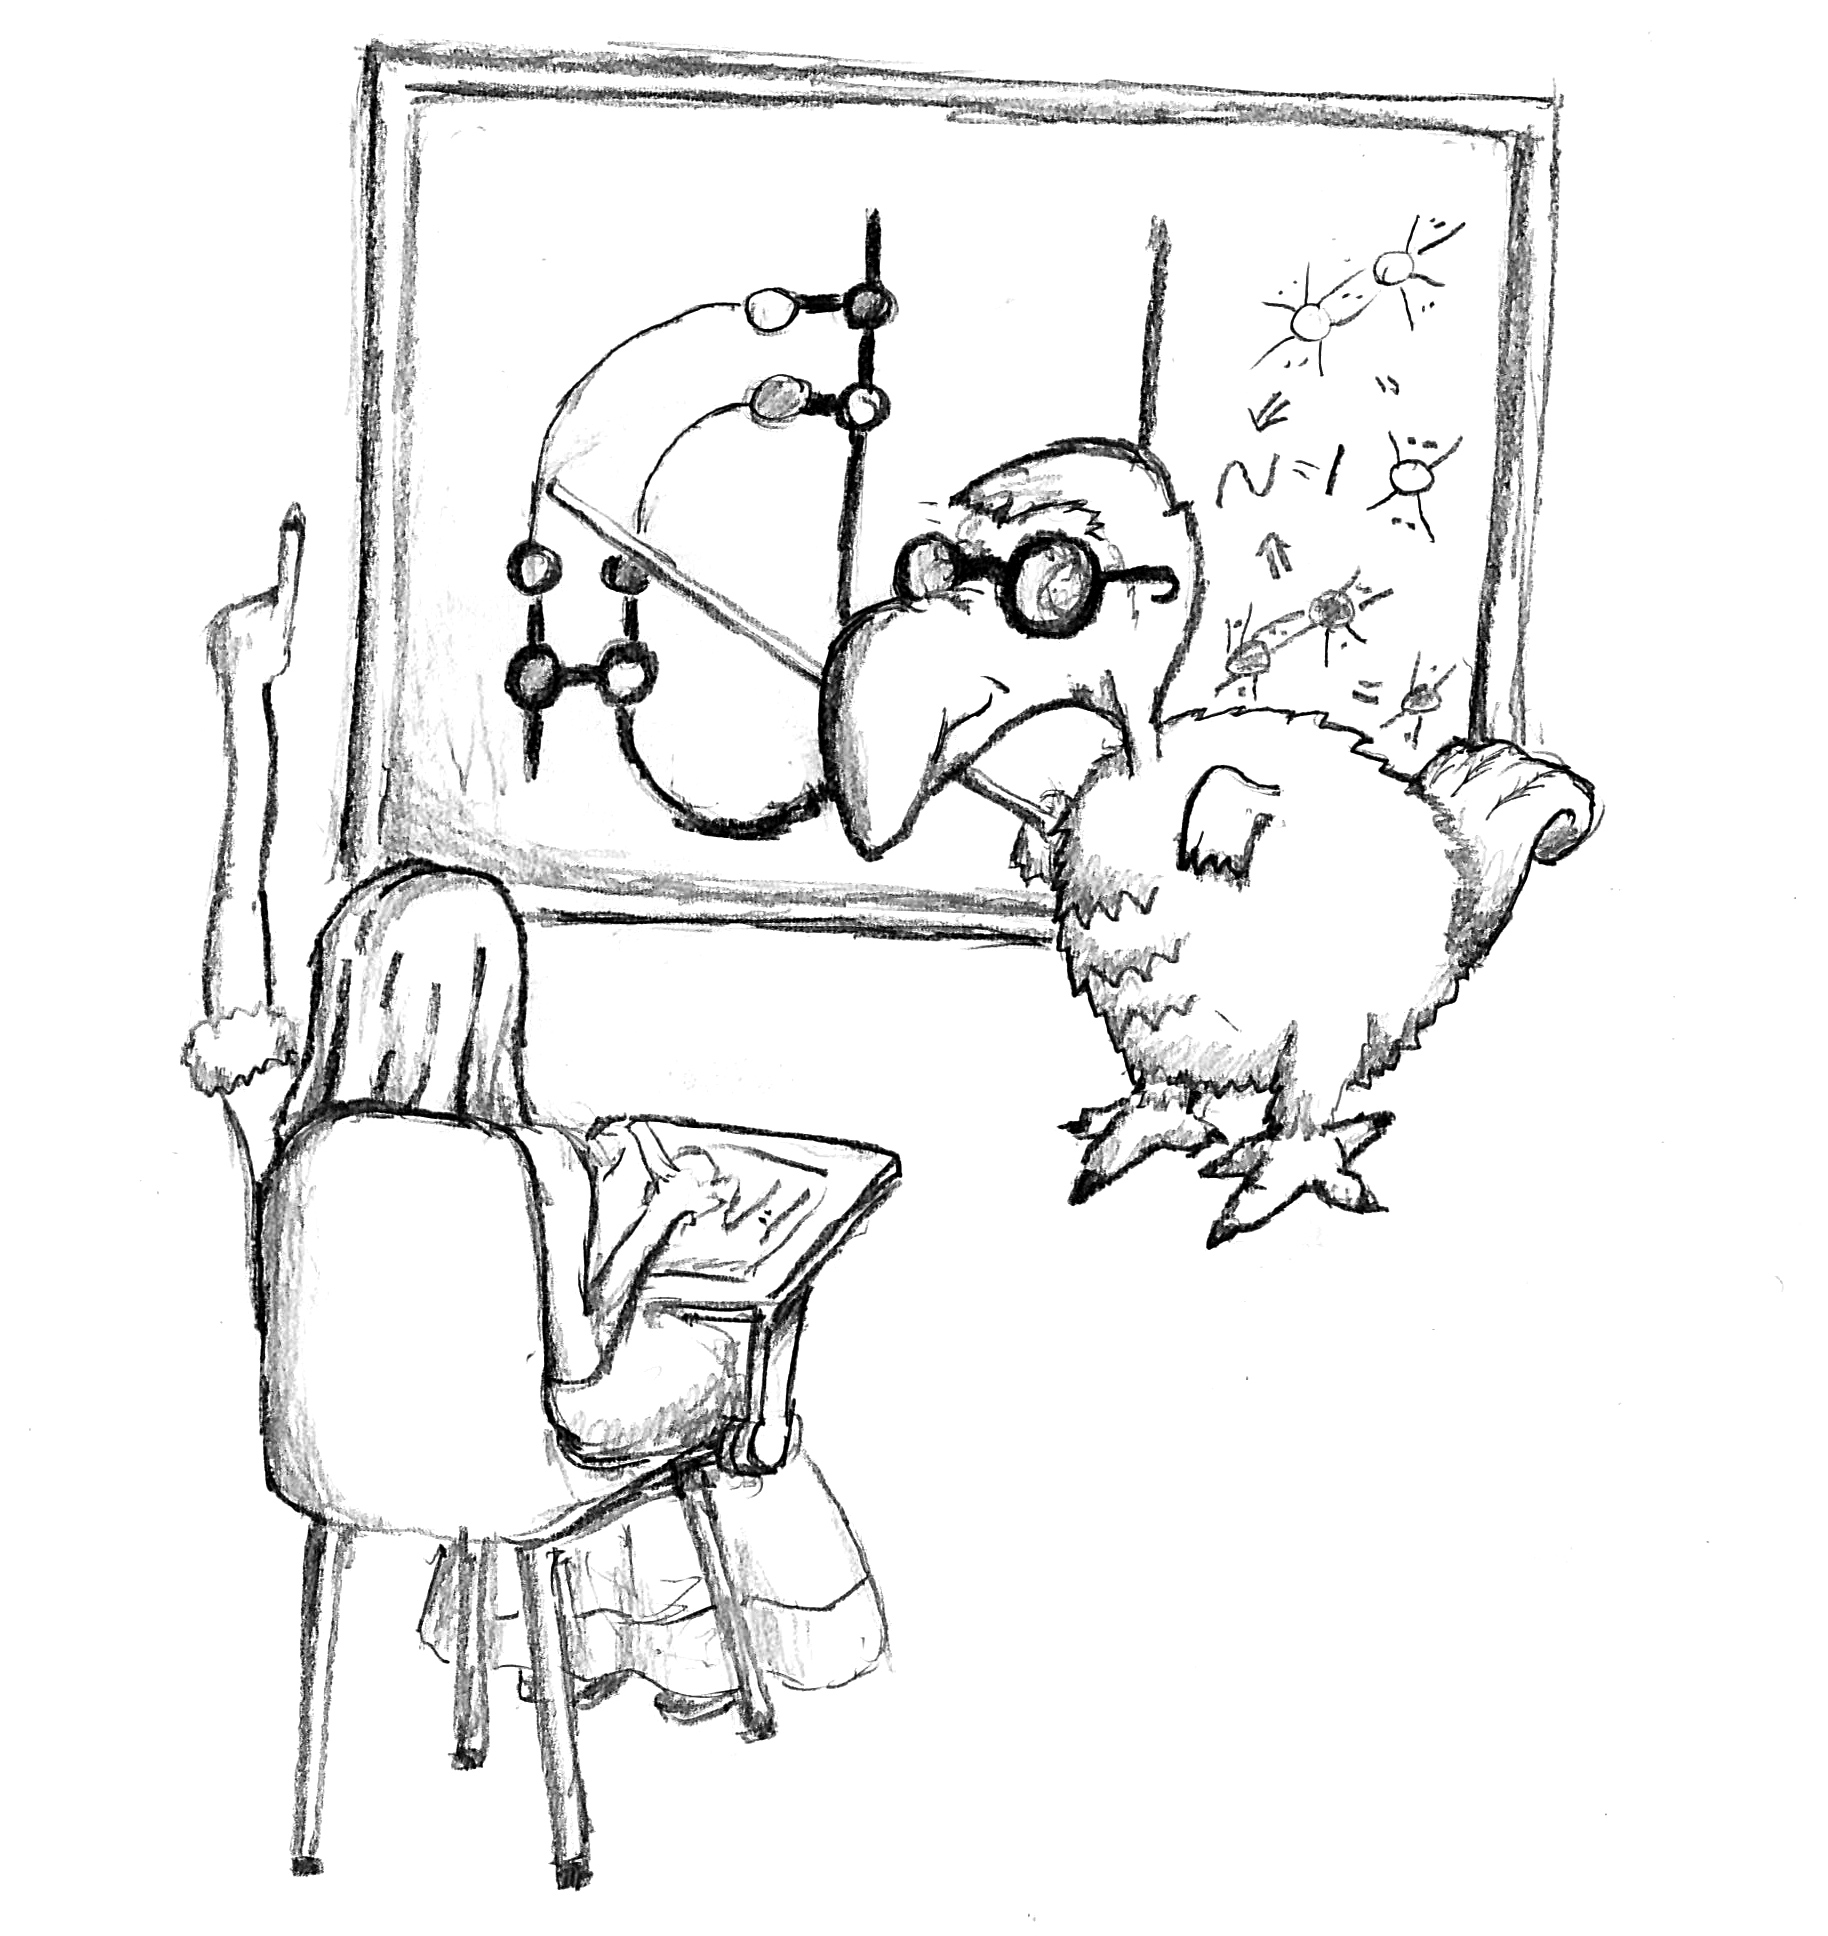
\includegraphics[width=0.5\textwidth]{dave-teach.jpg}
% \end{center}

%\section{Some remaining challenges}%%%%%%%%%%%% 
%
%\bR ... more insights in the utility of rules, and results on rewrite strategies given that we don't have a confluent system ... \e
%
%\bR ... automated theorem generation: new results about physics that would enough to warrant publication independent of being automatically generated; e.g.~about multi-party entanglement using ZW-calculus ... \e

\bibliographystyle{plain}
\bibliography{main}

\end{document} 
